\section{Integration/Discretization error tests}
GIT \texttt{b6fa1d8611cf968aa9f0a9f32d684879dceffa54}, tag \texttt{integerror\_begin}

This experiment investigates the influence of discretization and integration order for sub-element inhomogeneous material laws.
The basic question is to see whether the three-point gauss integration rule is sufficiently accurate for in-element inhomogeneous material laws.
We integrate using the \texttt{ode15i} \ML-solver (AbsTol $1E-5$, RelTol $1E-5$) over $t\in[0,T], T=99$ with $\Delta t = 1 [ms]$. 

The model default parameter configuration is
% PrintTable generated on 18-May-2015 14:11:49
% Export settings: TexMathModeDetection 1, HasHeader 1, HasRowHeader 1, StripInsertedTabChars 1, IsPDF 0, TightPDF 1
\begin{table}[!hb]
	\centering
	\def\arraystretch{1.3}
	\begin{tabular}{rll}
		Parameter 				& Value		& Index\\
		\hline\\
		viscosity				& $0.1$		& $1$\\
		alpha ramp time			& $0$		& $2$\\
		neumann pressure			& $0.1$		& $3$\\
		mean input current			& $0$		& $4$\\
		muscle passive $b_1$			& $2.756e-05$	& $5$\\
		muscle passive $d_1$			& $43.373$	& $6$\\
		tendon passive 1 $[b_1/\la_0]$		& $1.0207$	& $7$\\
		tendon passive 2 $[d_1/M]$			& $163789$	& $8$\\
		muscle mooney-rivlin $c^M_{10}$		& $0.0356$	& $9$\\
		muscle mooney-rivlin $c^M_{01}$		& $0.00386$	& $10$\\
		tendon mooney-rivlin $c^T_{10}$		& $2310$	& $11$\\
		tendon mooney-rivlin $c^T_{01}$		& $0.00115$	& $12$\\
		$P_{max}$					& $0.3$		& $13$\\
		force-length $p_1$ ($\la_0/width/...$)	& $2.05$	& $14$\\
	\end{tabular}
\end{table}
\subsection{Inhomogeneous sub-element material law}
As the material laws are sampled at each Gauss point only, the material laws can be prescribed differently at each point.
We differ between muscle and tendon material, indicated by $\theta(\pmp) \in [0,1]$ (Element $m$, point $p$), where $\theta=0$ stands for muscle only.  
The isotropic material law used at each Gauss point $\pmp$ is Mooney-Rivlin via 
\begin{align}
	2(\tilde c_{10}(\pmp) &+ \vI \tilde c_{01}(\pmp))- 2\tilde c_{01}(\pmp)\vC,\\
	 \tilde c_{10}(\pmp) &= \theta(\pmp) c^M_{10}(\pmp) + (1-\theta(\pmp))c^T_{10}(\pmp),\\
	 \tilde c_{01}(\pmp) &= \theta(\pmp) c^M_{01}(\pmp) + (1-\theta(\pmp))c^T_{01}(\pmp).
\end{align}
For anisotropic material (see Section \ref{sssec:aniso_stress}), we use the classic Markert-Law \cite{Markert2005}
for muscle material and a cubic/linear function
\begin{align}
	\theta(\pmp)b_1\la^{-1}(\la^{d_1} - 1) + (1-\theta(\pmp))f_{\la_0,M}(\la)
\end{align}
with
\begin{align}
	f_{\la_0,M}(\la) &= \begin{cases}
		f_{\la_0,M}(\la_0) + M(\la-\la_0) & \la > \la_0\\
		\frac{M}{3(\la_0-1)^2}(\la^3+3\la^2+3\la-1)& 0 \leq \la \leq \la_0
	\end{cases}
\end{align}
Here, the stretch $\la_0$ denotes the switch from cubic to linear function with derivative $M$.
The polynomial is fitted in a way that the derivative at $\la_0$ equals $M$, i.e. $f_{\la_0,M}\in C^1$.
Figure \ref{fig:aniso_pressure} depicts the anisotropic pressure contributions for muscle and tendon material.
\begin{figure}[!ht]
	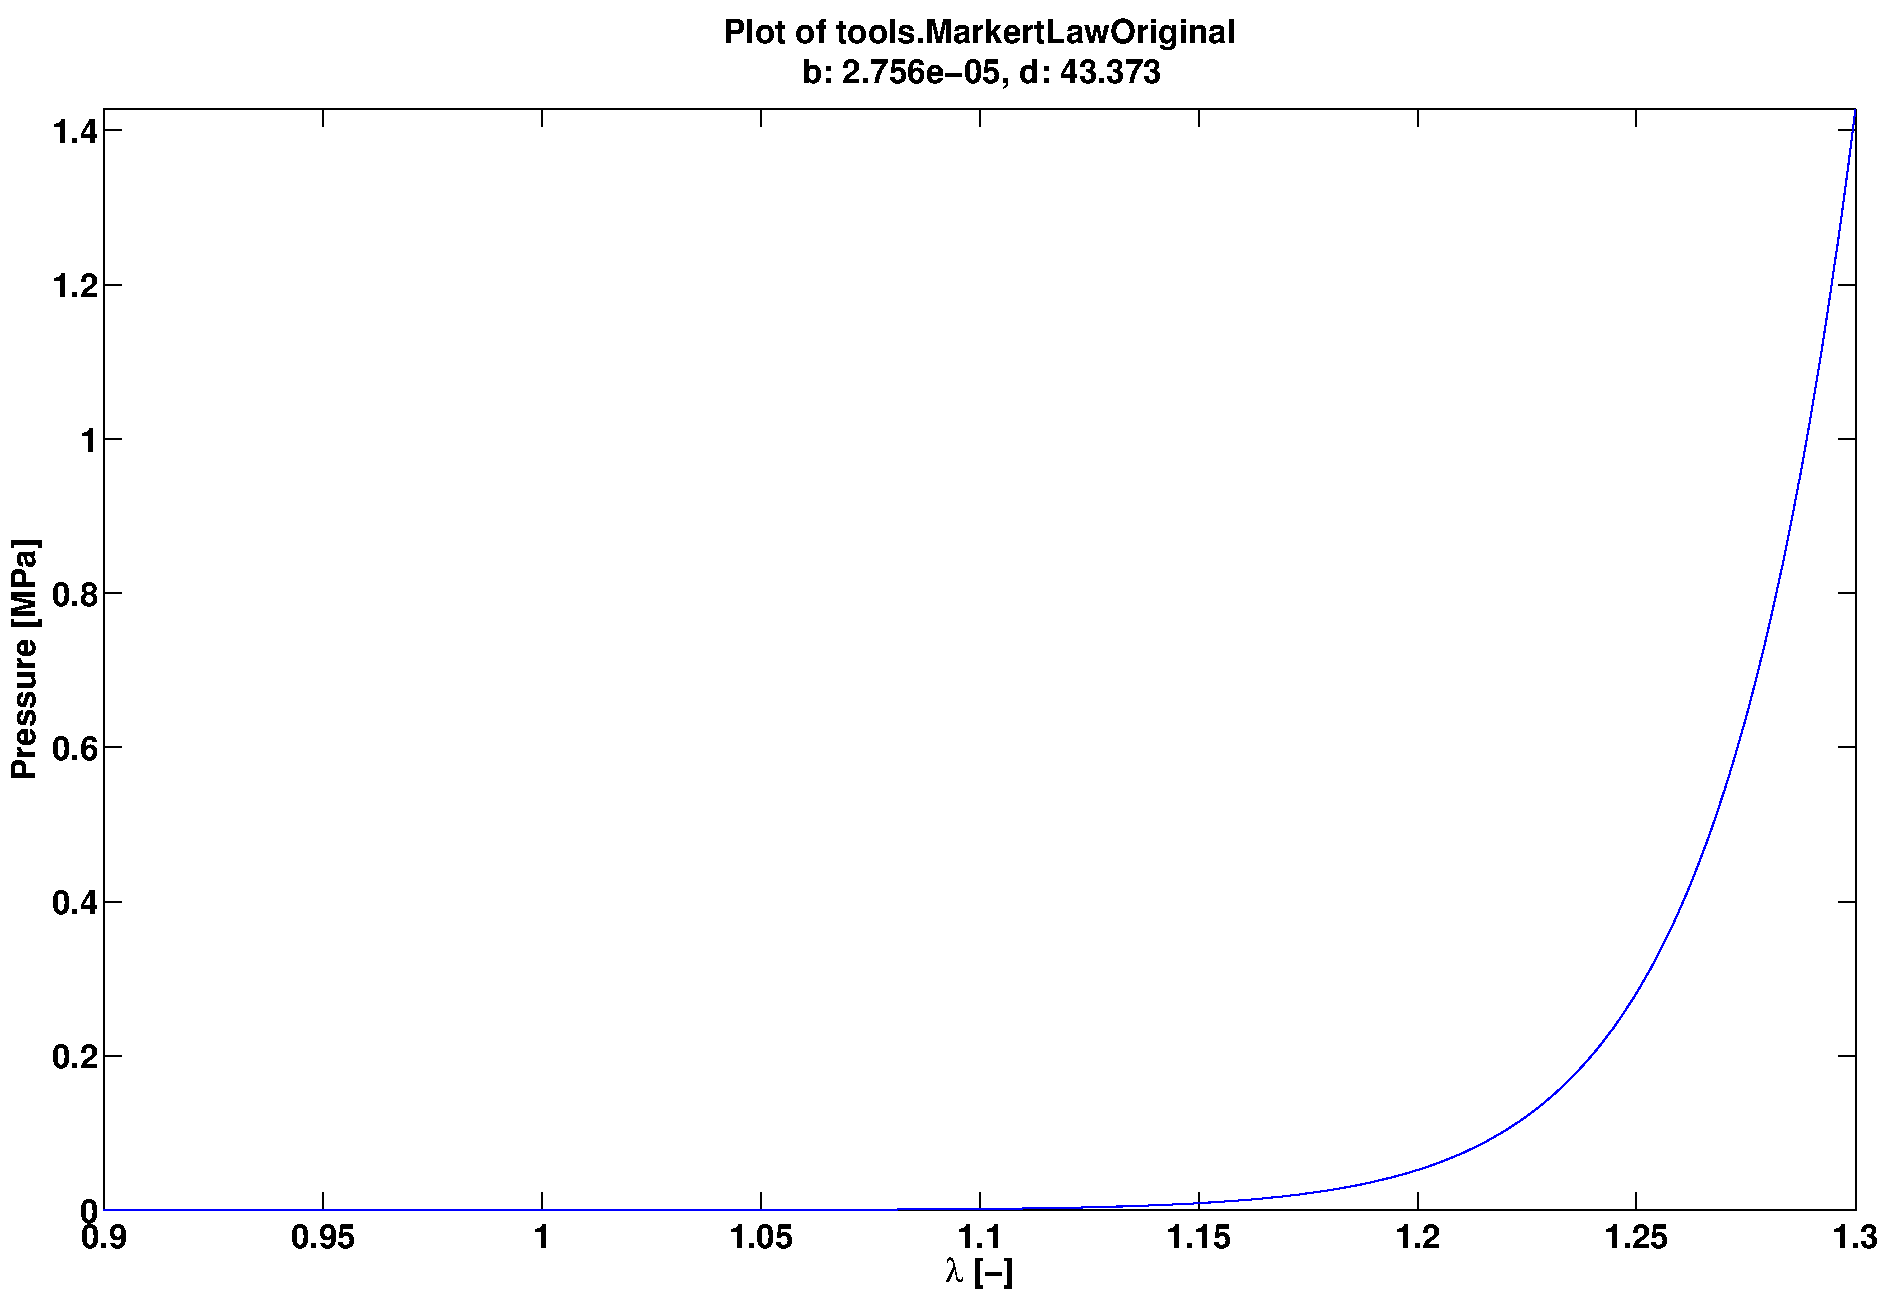
\includegraphics[width=\half]{geo_1_aniso_tools_MarkertLawOriginal}
	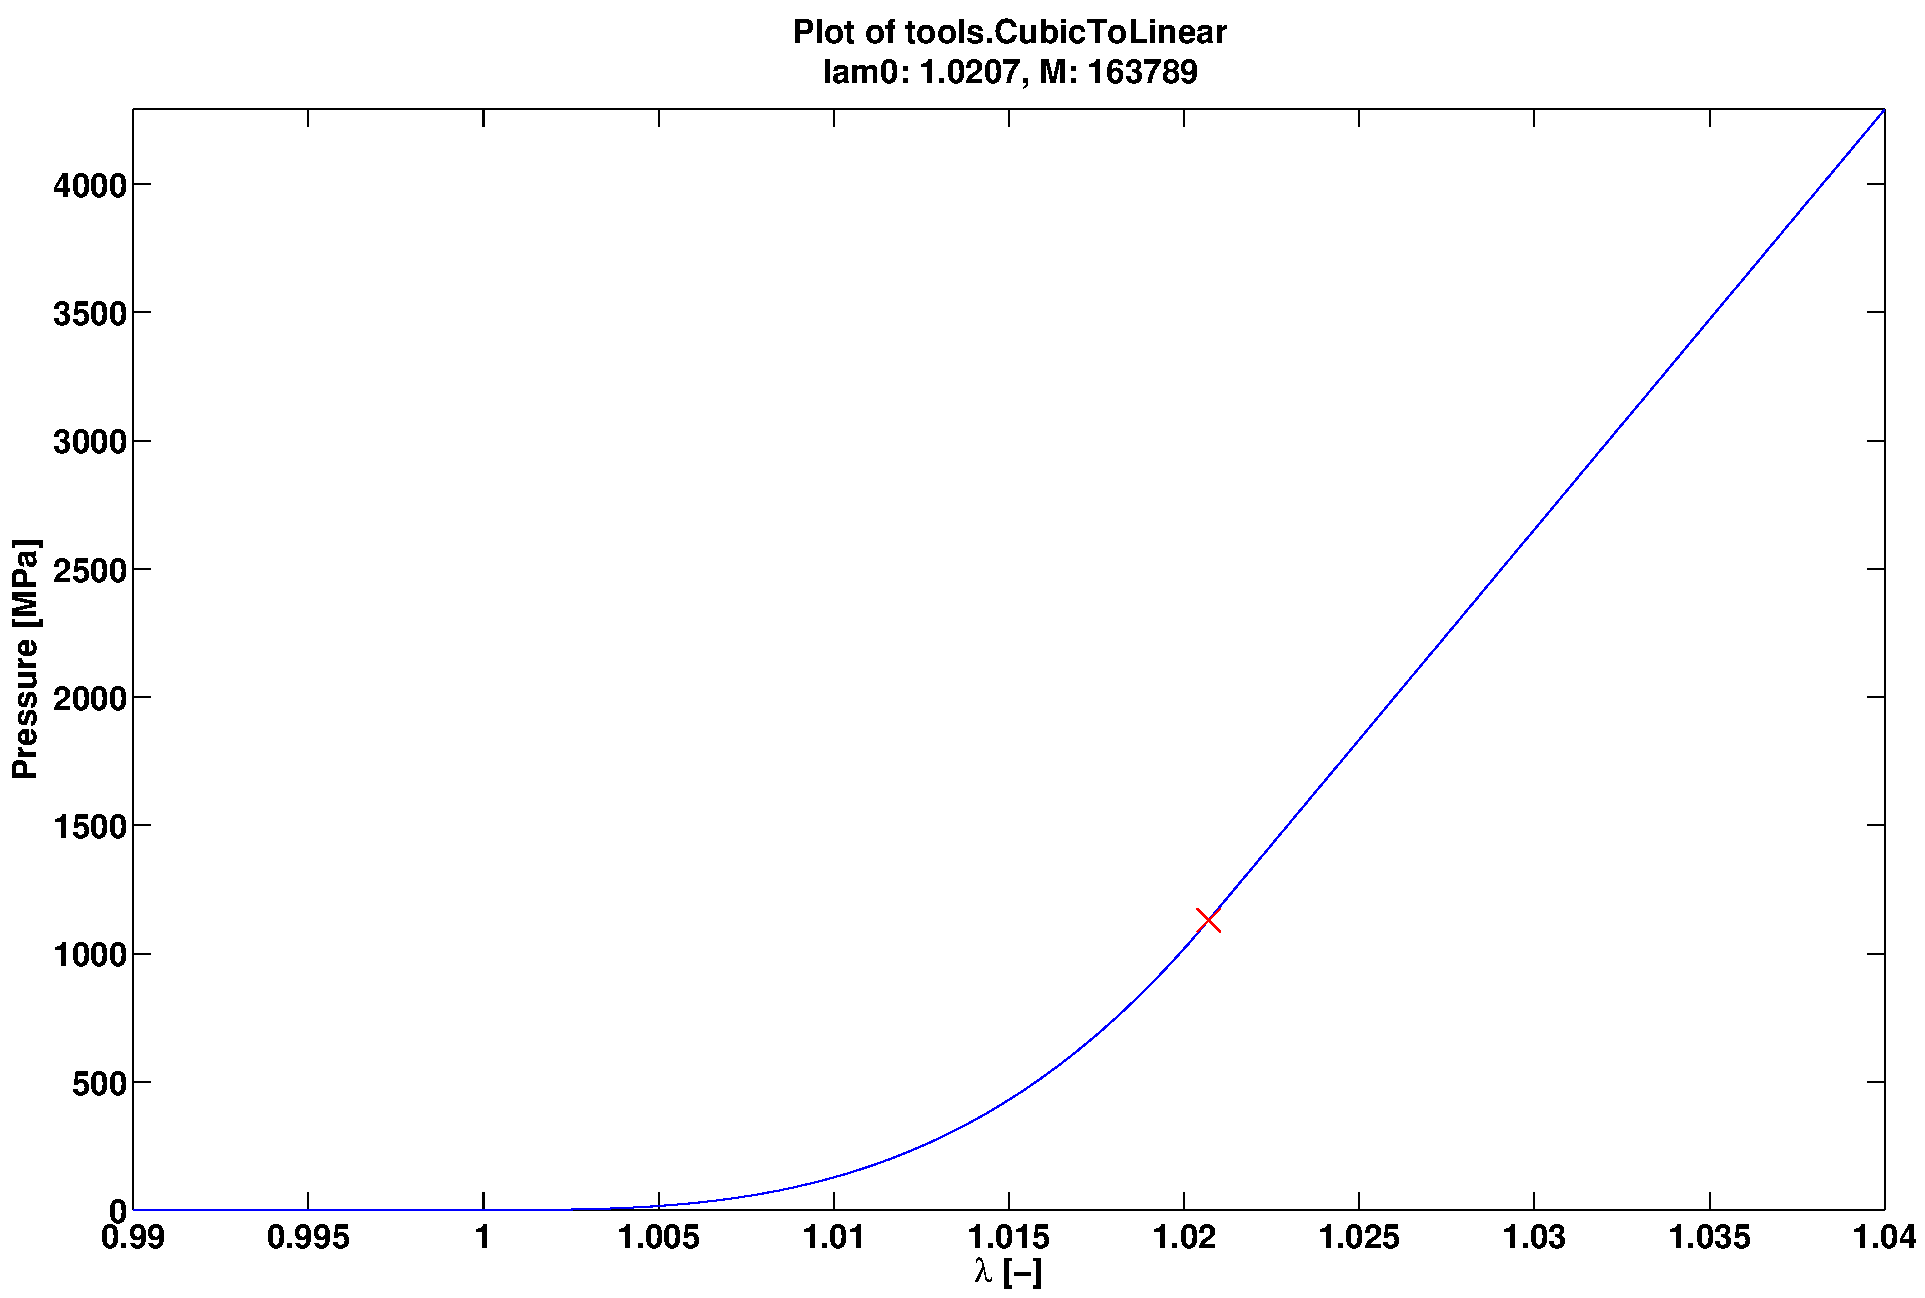
\includegraphics[width=\half]{geo_1_aniso_tools_CubicToLinear}
	\caption{Anisotropic pressure curves for muscle and tendon material. Left: Muscle, right: Tendon $f_{\la_0,M}$ }
	\label{fig:aniso_pressure}
\end{figure}
\subsection{Geometry setup}
We define ten configurations with increasing tendon material at the left side
\begin{align}
	\theta_i(X) = \begin{cases}
		0 & X_1 > 3\\
		i/9 & X_1 <= 3\\
	\end{cases}, && X\in\Omega,~i=0\ldots 9.
\end{align}
\subsubsection{One element discretization}
The geometry setup is a simple hexahedral element $\Omega = [0,10]^3~[mm]$ with quadratic ansatz functions, e.g. $27$ Nodes.
Figure \ref{fig:geo1} illustrates the different geometric configurations.
\begin{figure}[!ht]
	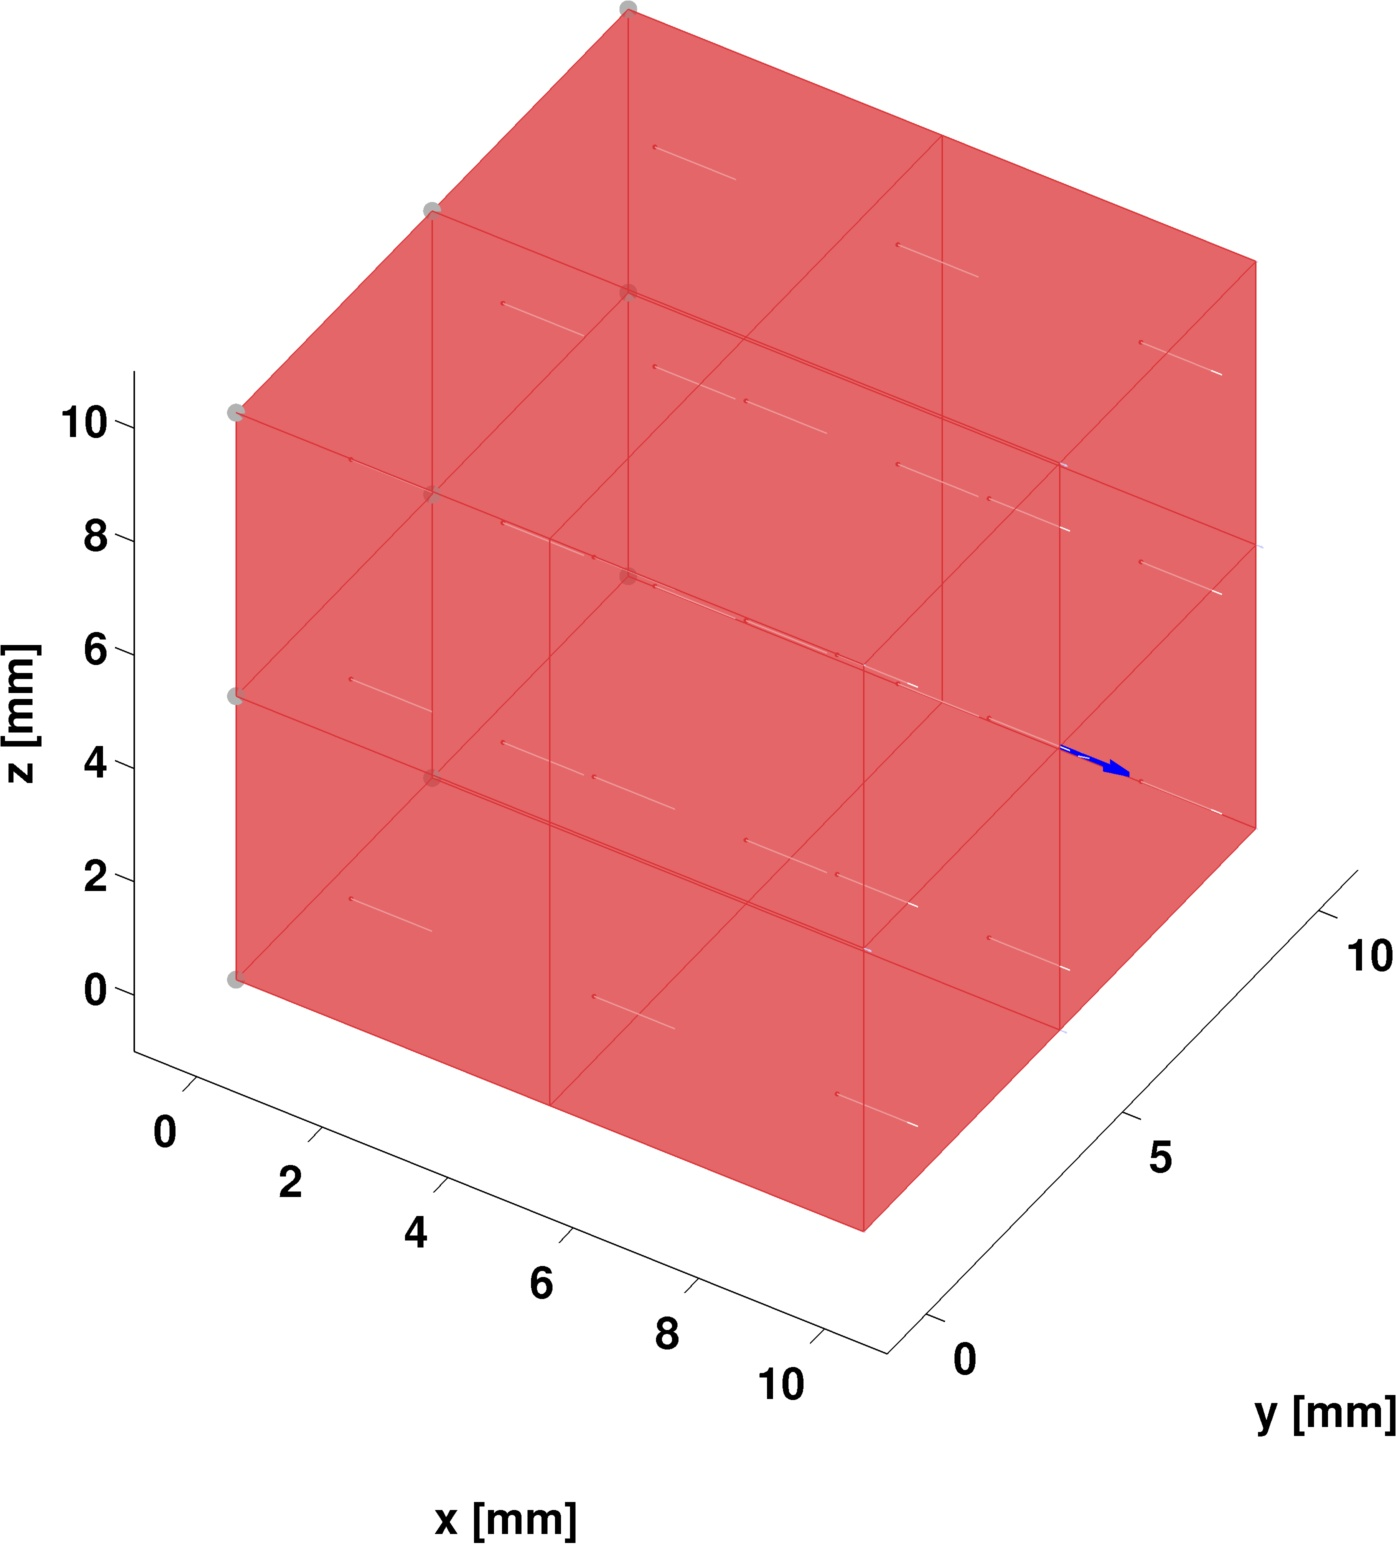
\includegraphics[width=\third]{geo_1_conf_1_gauss_3_geo}
% 	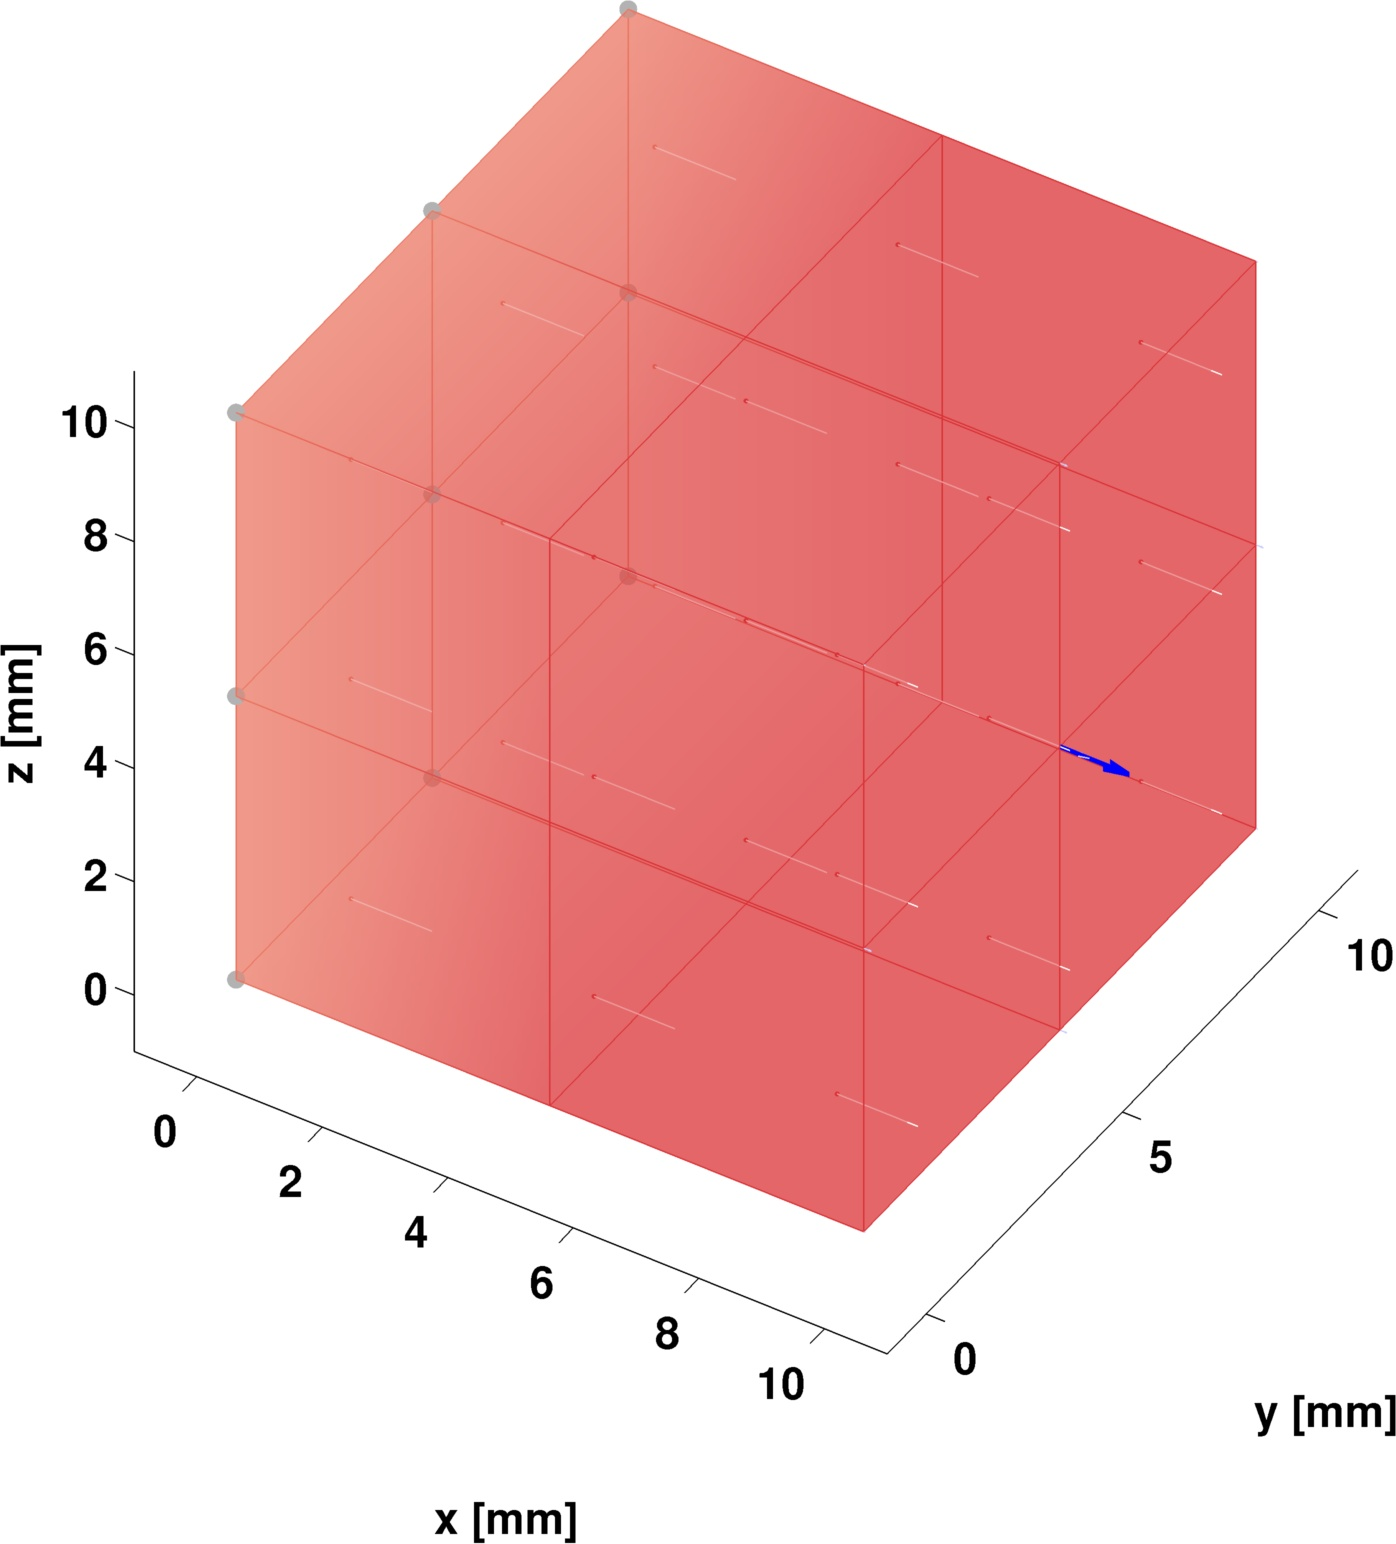
\includegraphics[width=\third]{geo_1_conf_5_gauss_3_geo}
% 	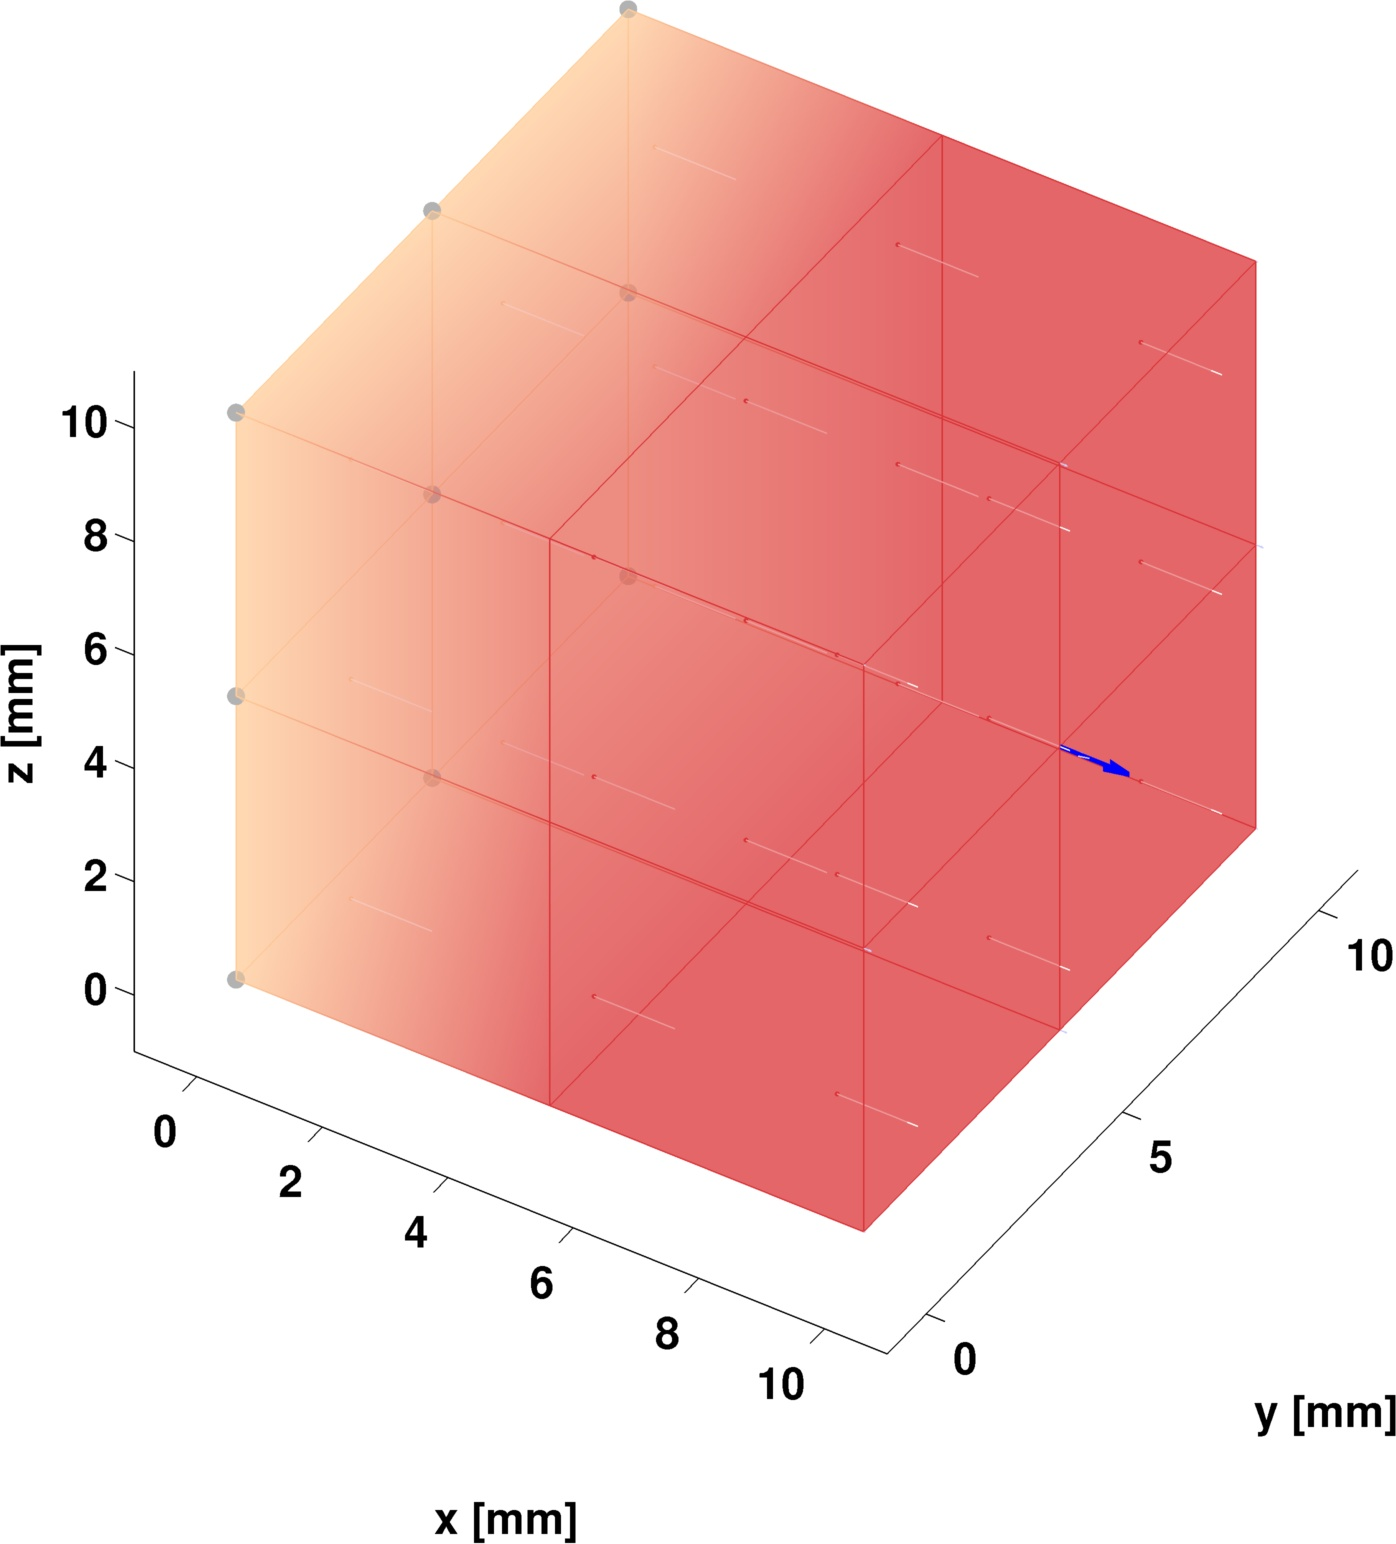
\includegraphics[width=\third]{geo_1_conf_10_gauss_3_geo}\\
% 	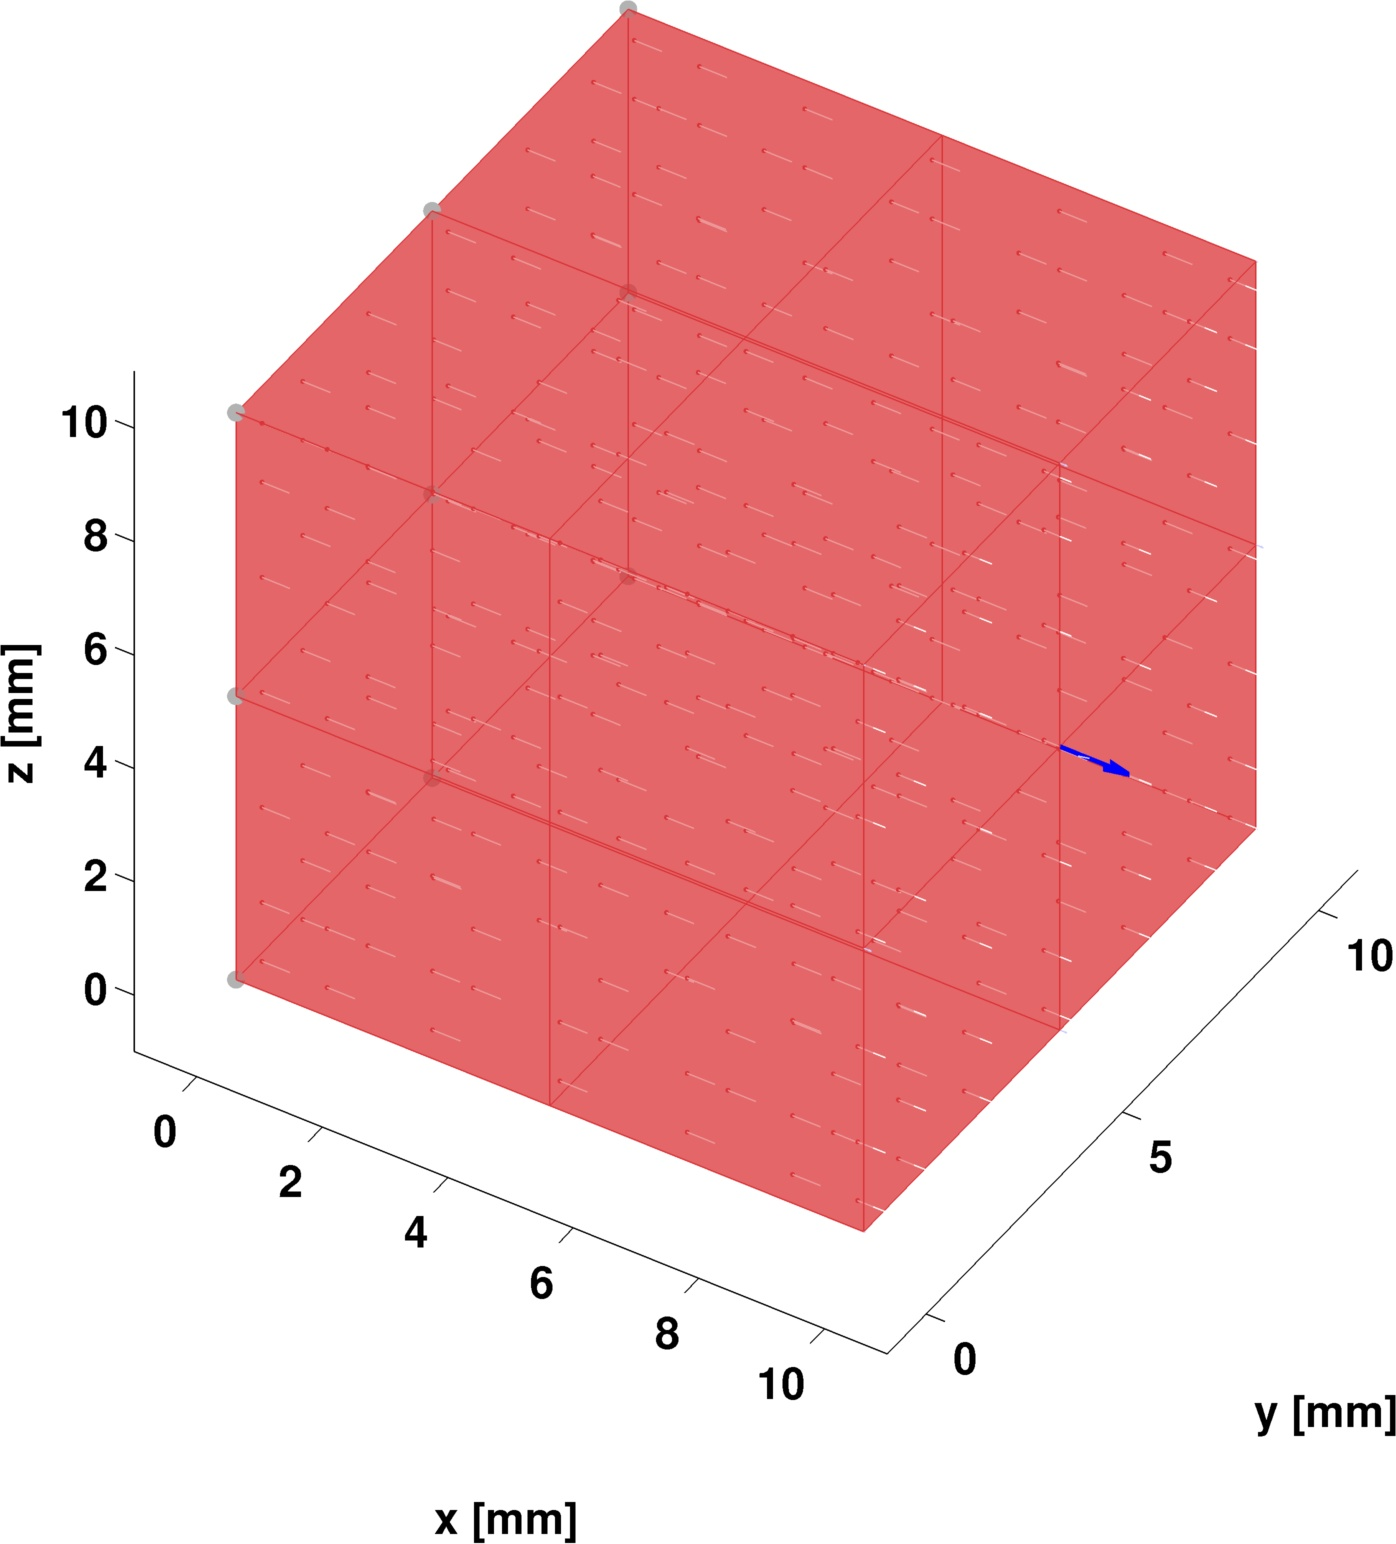
\includegraphics[width=\third]{geo_1_conf_1_gauss_7_geo}
% 	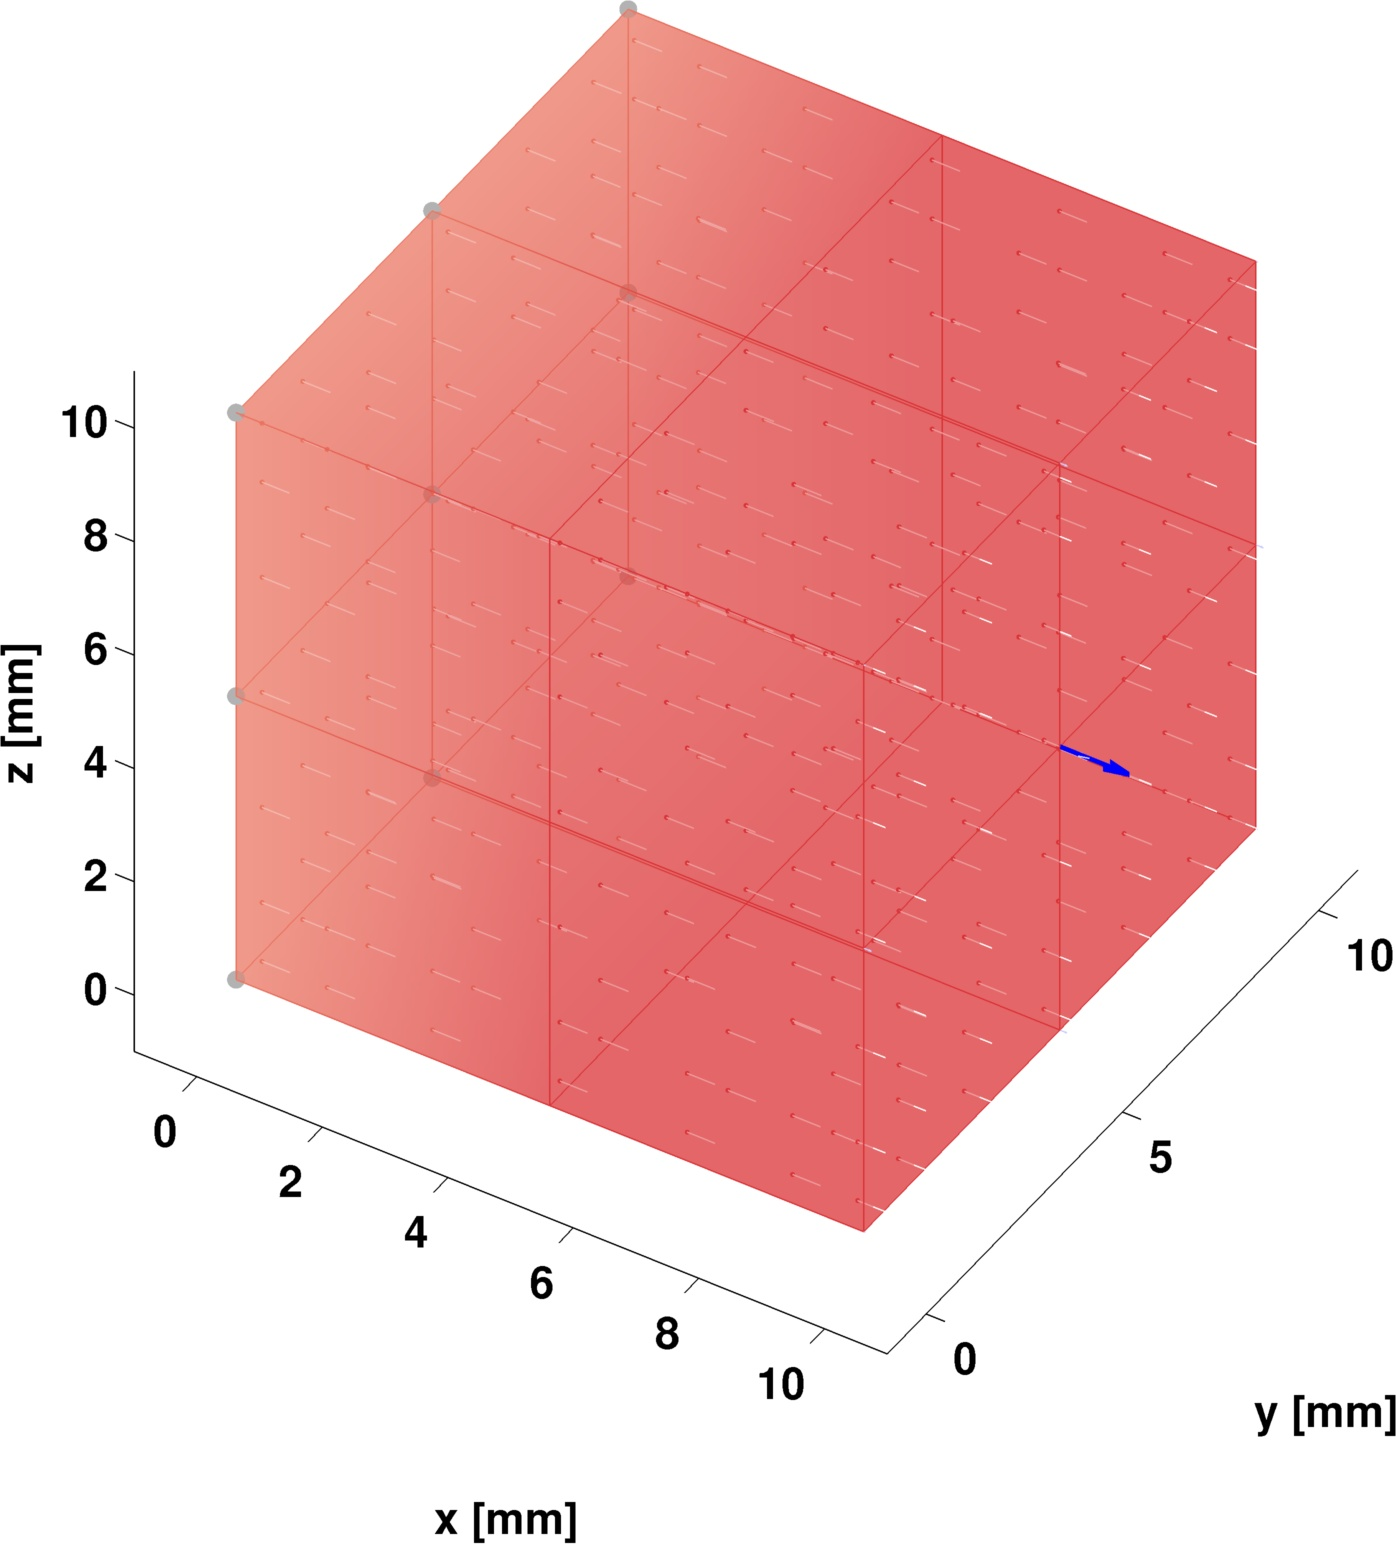
\includegraphics[width=\third]{geo_1_conf_5_gauss_7_geo}
% 	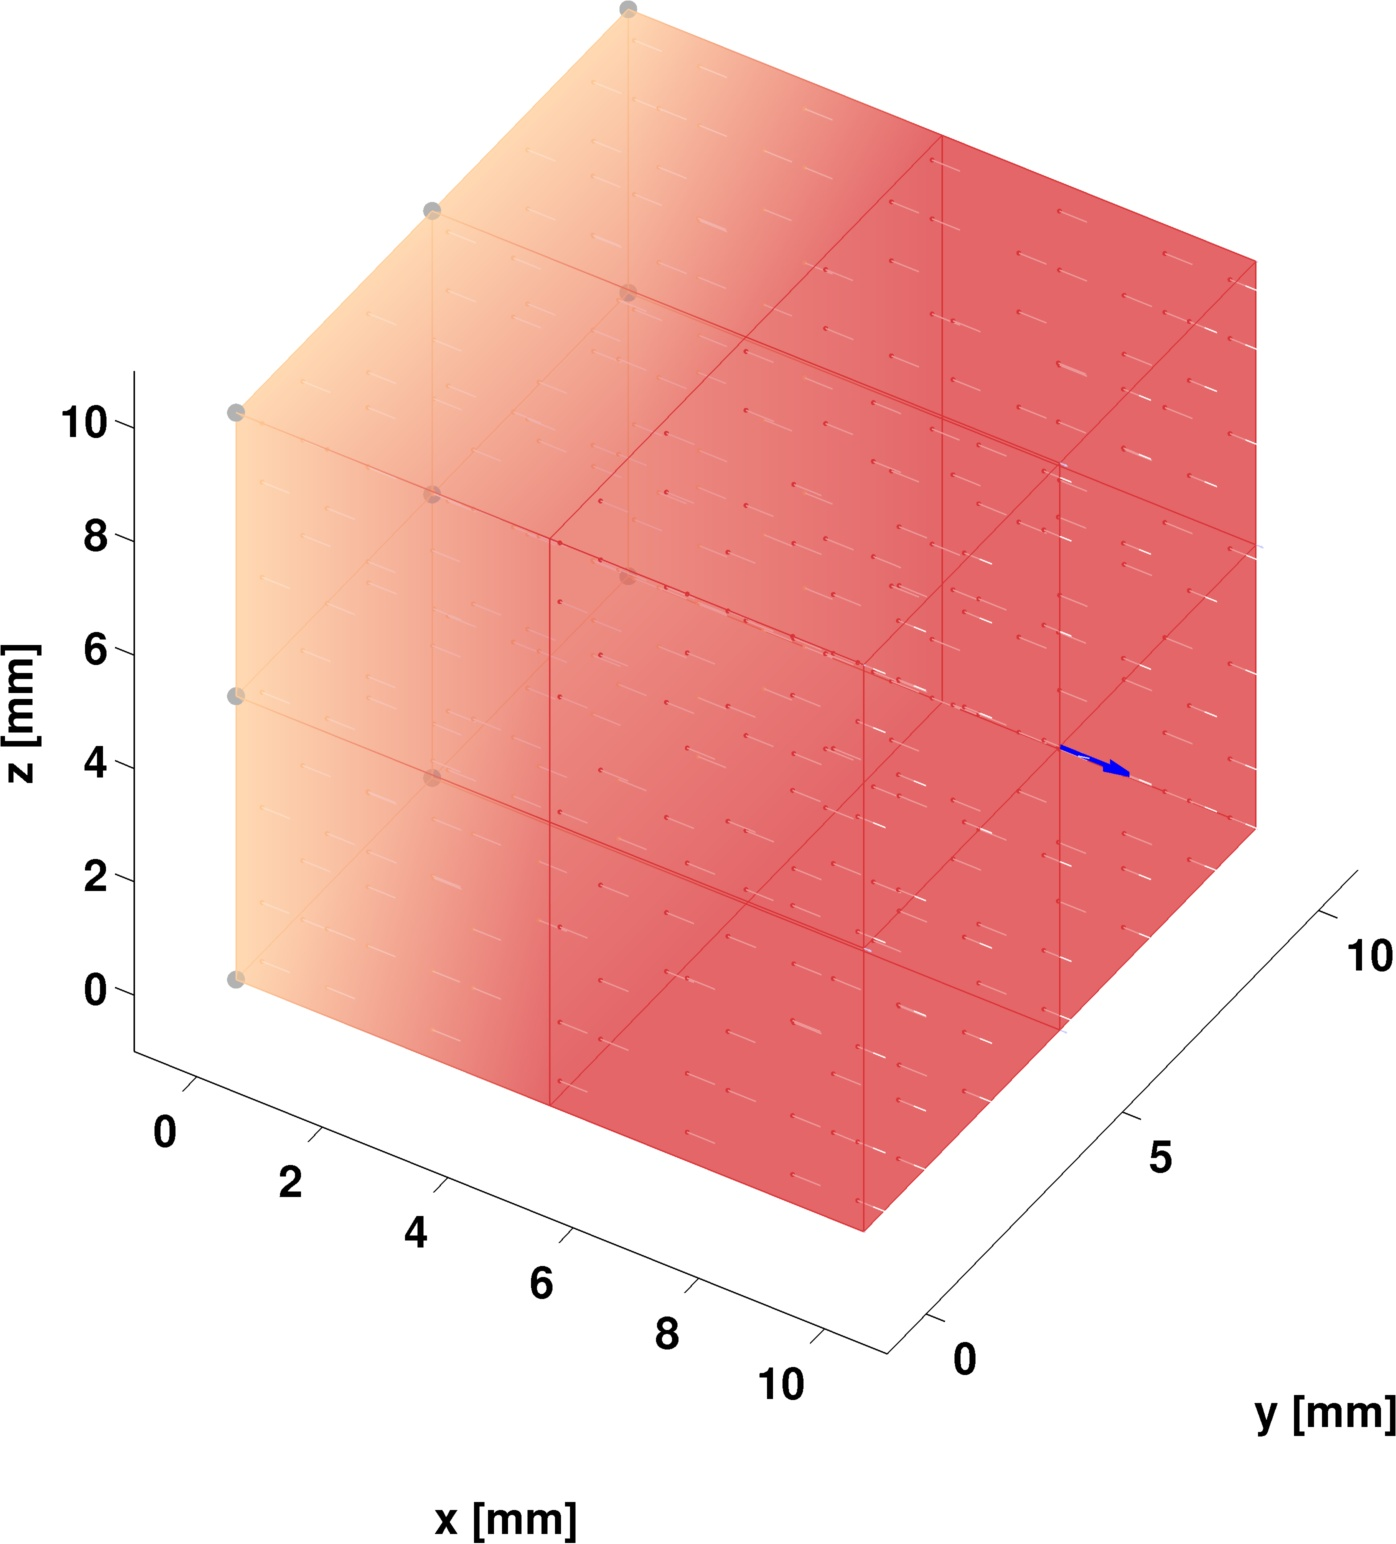
\includegraphics[width=\third]{geo_1_conf_10_gauss_7_geo}\\
% 	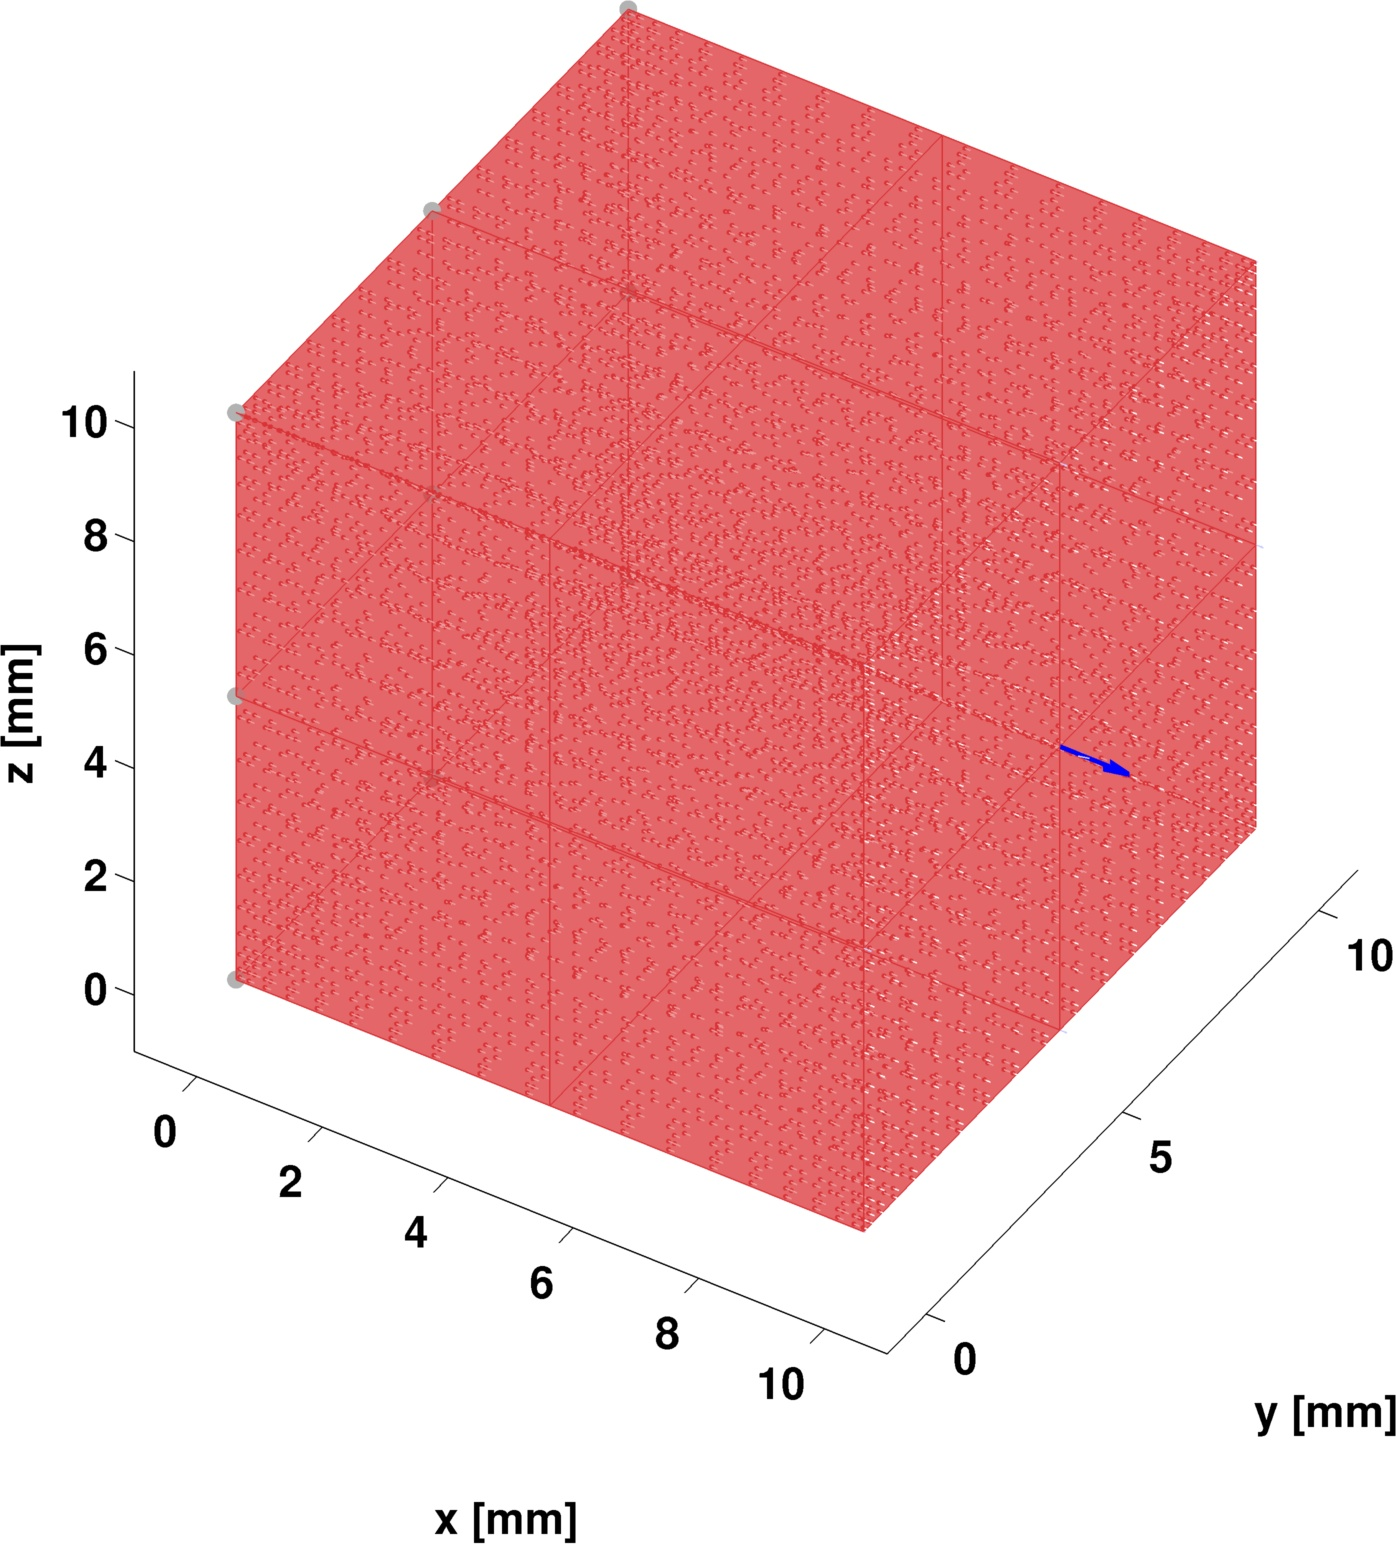
\includegraphics[width=\third]{geo_1_conf_1_gauss_20_geo}
% 	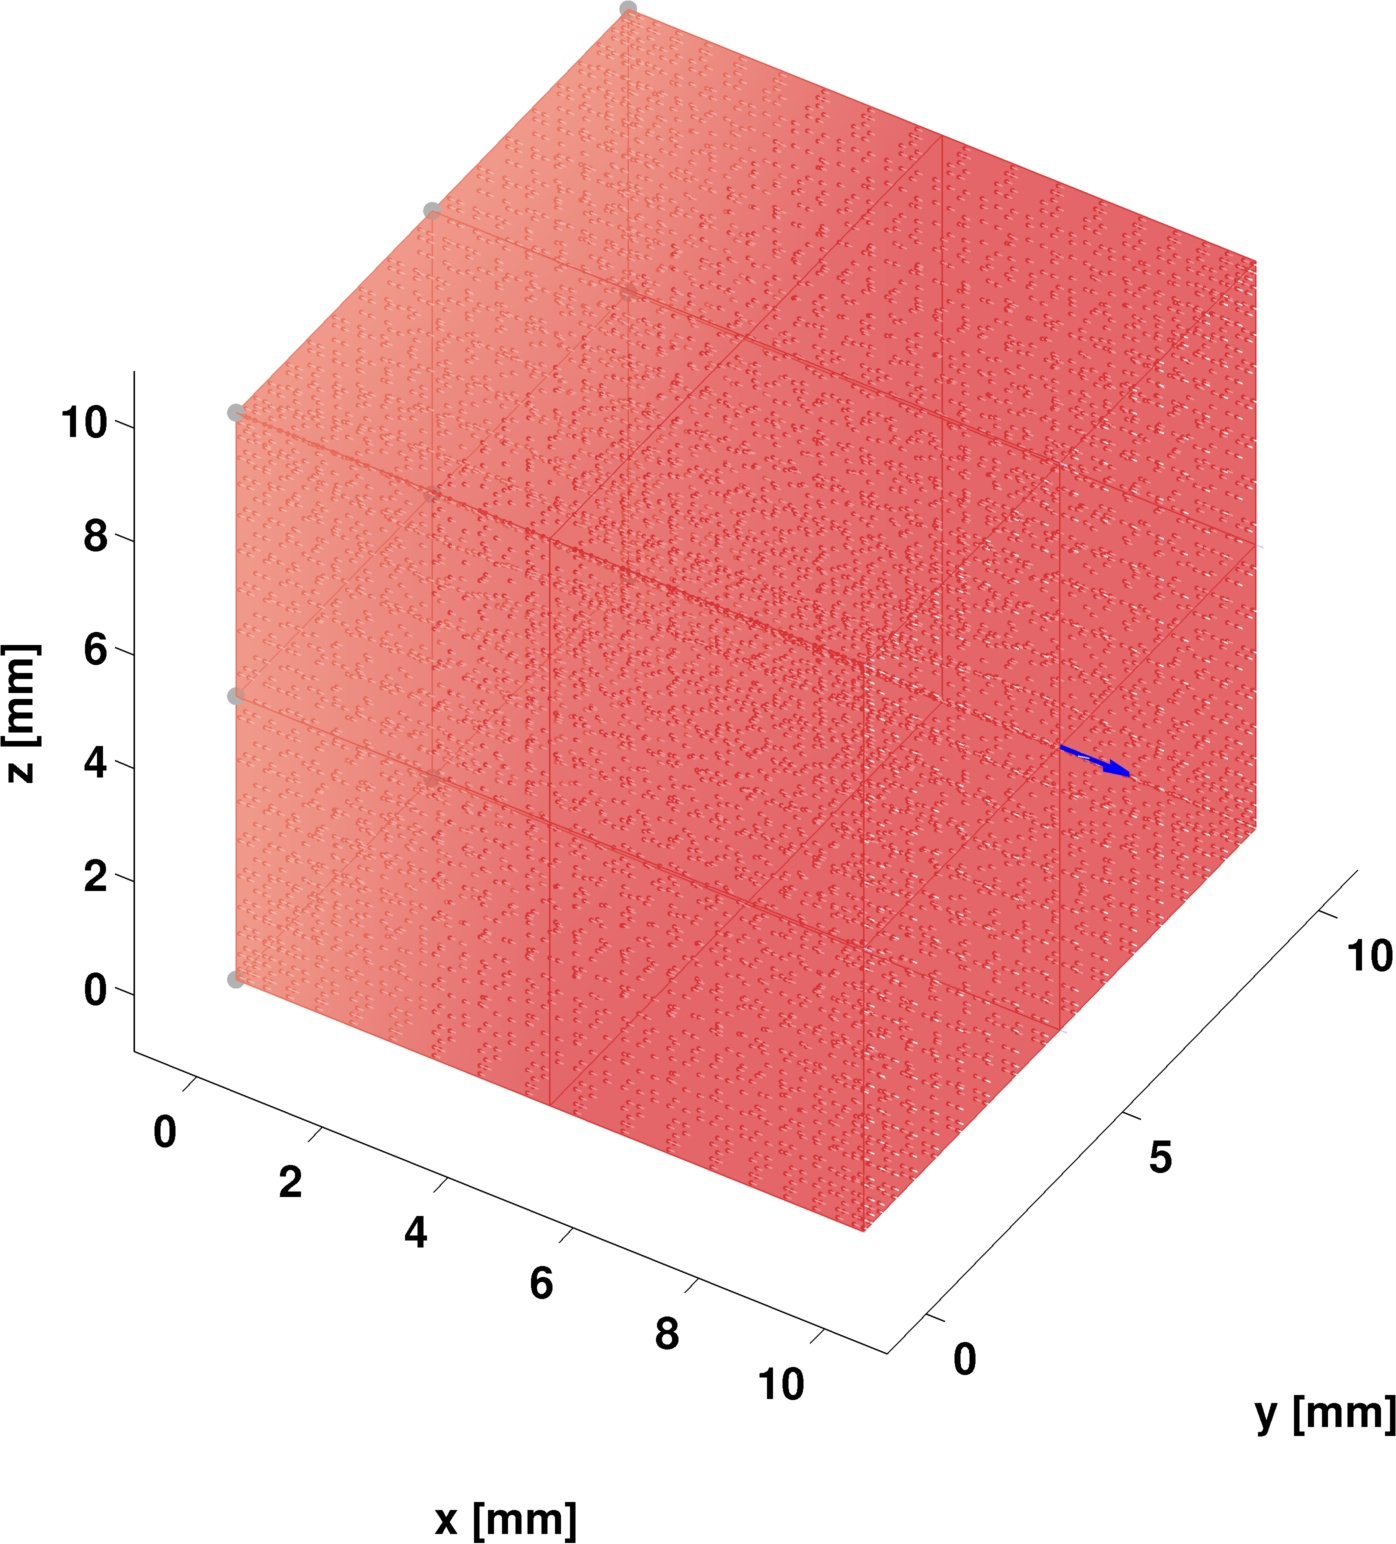
\includegraphics[width=\third]{geo_1_conf_5_gauss_20_geo}
% 	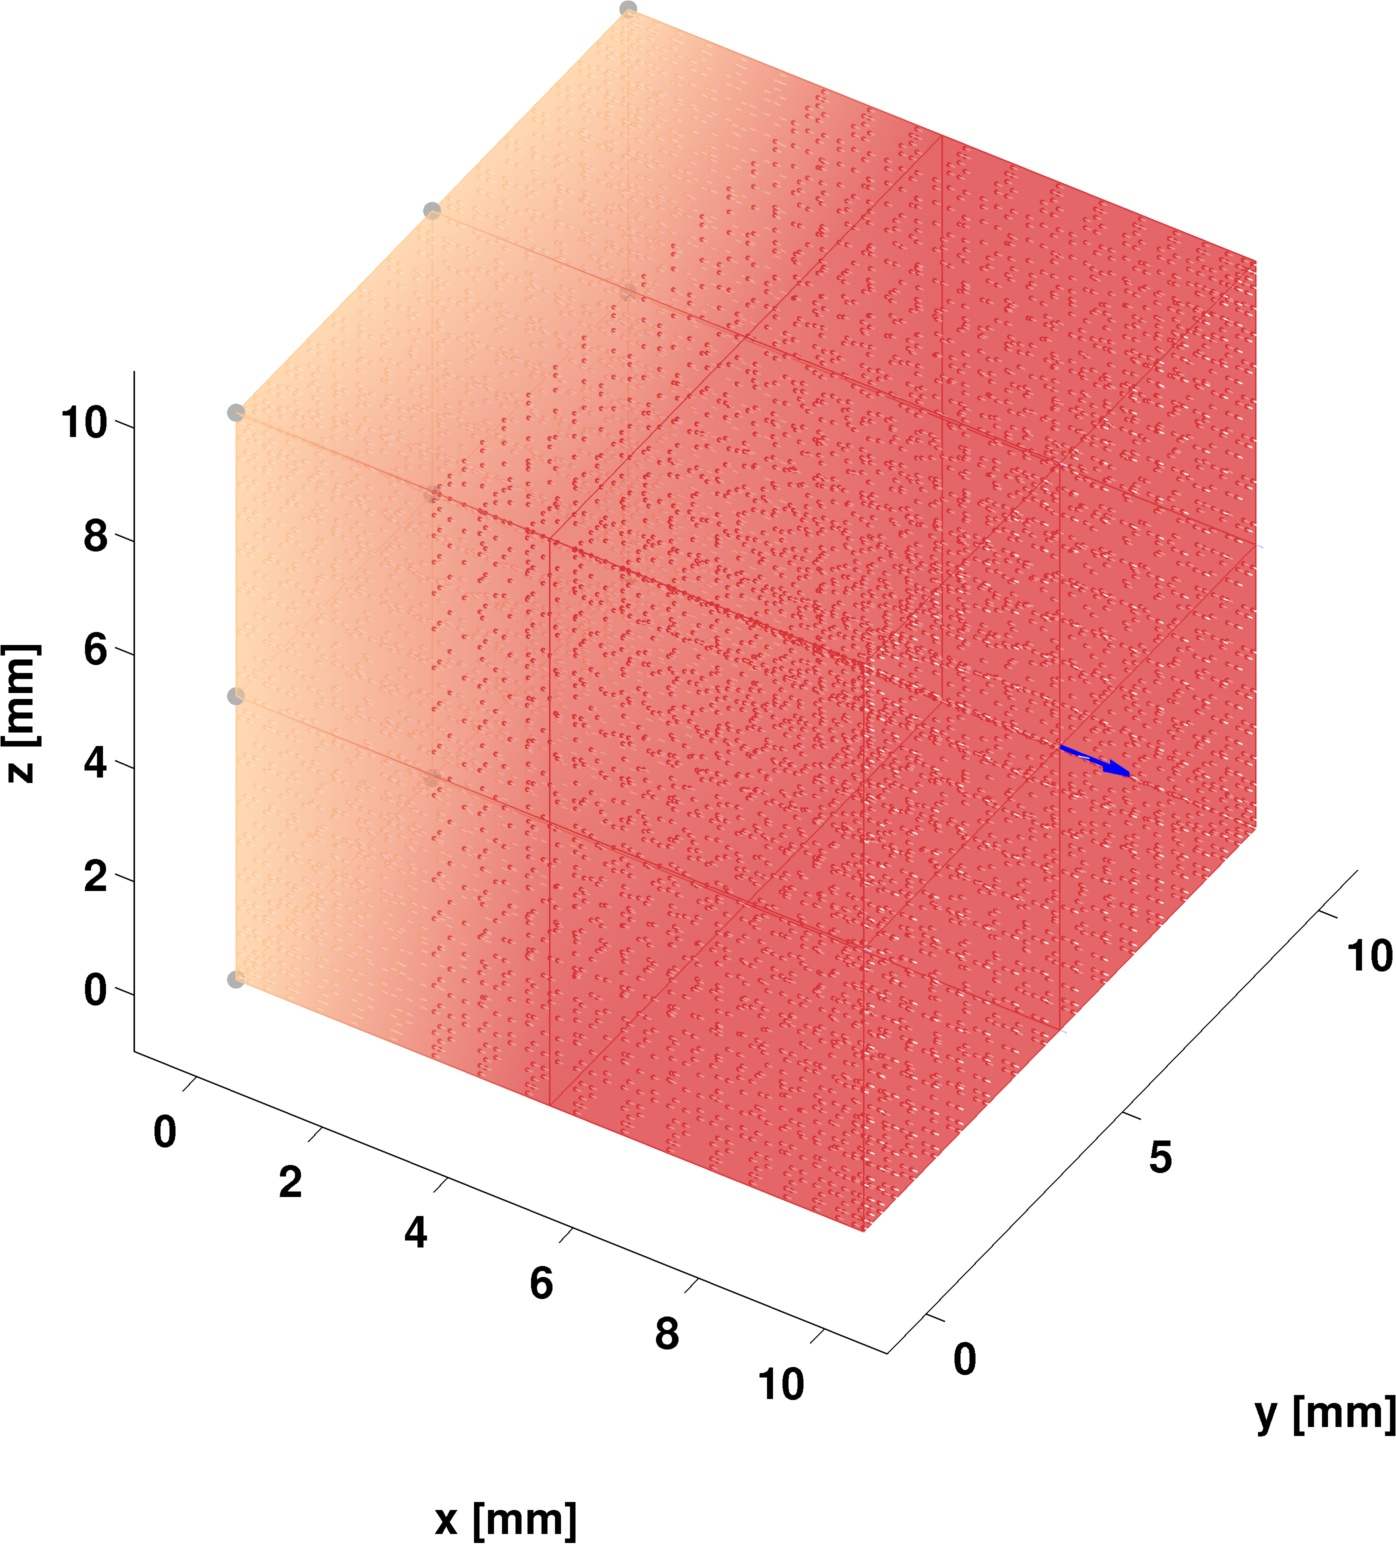
\includegraphics[width=\third]{geo_1_conf_10_gauss_20_geo}\\
	\caption{Experiment geometry for case 1: One element. 
	Left to right: configurations $\theta_1,\theta_5,\theta_{10}$, top to bottom: gauss integration rules $3,7,20$ points}
	\label{fig:geo1}
\end{figure}
\subsubsection{Two element discretization}
The second discretization has two elements over the same volume $\Omega$, albeit being split exactly at $x=3$, so that two elements
with each \textit{homogeneous} material laws are the result, see Figure \ref{fig:geo2}.
\begin{figure}[!ht]
	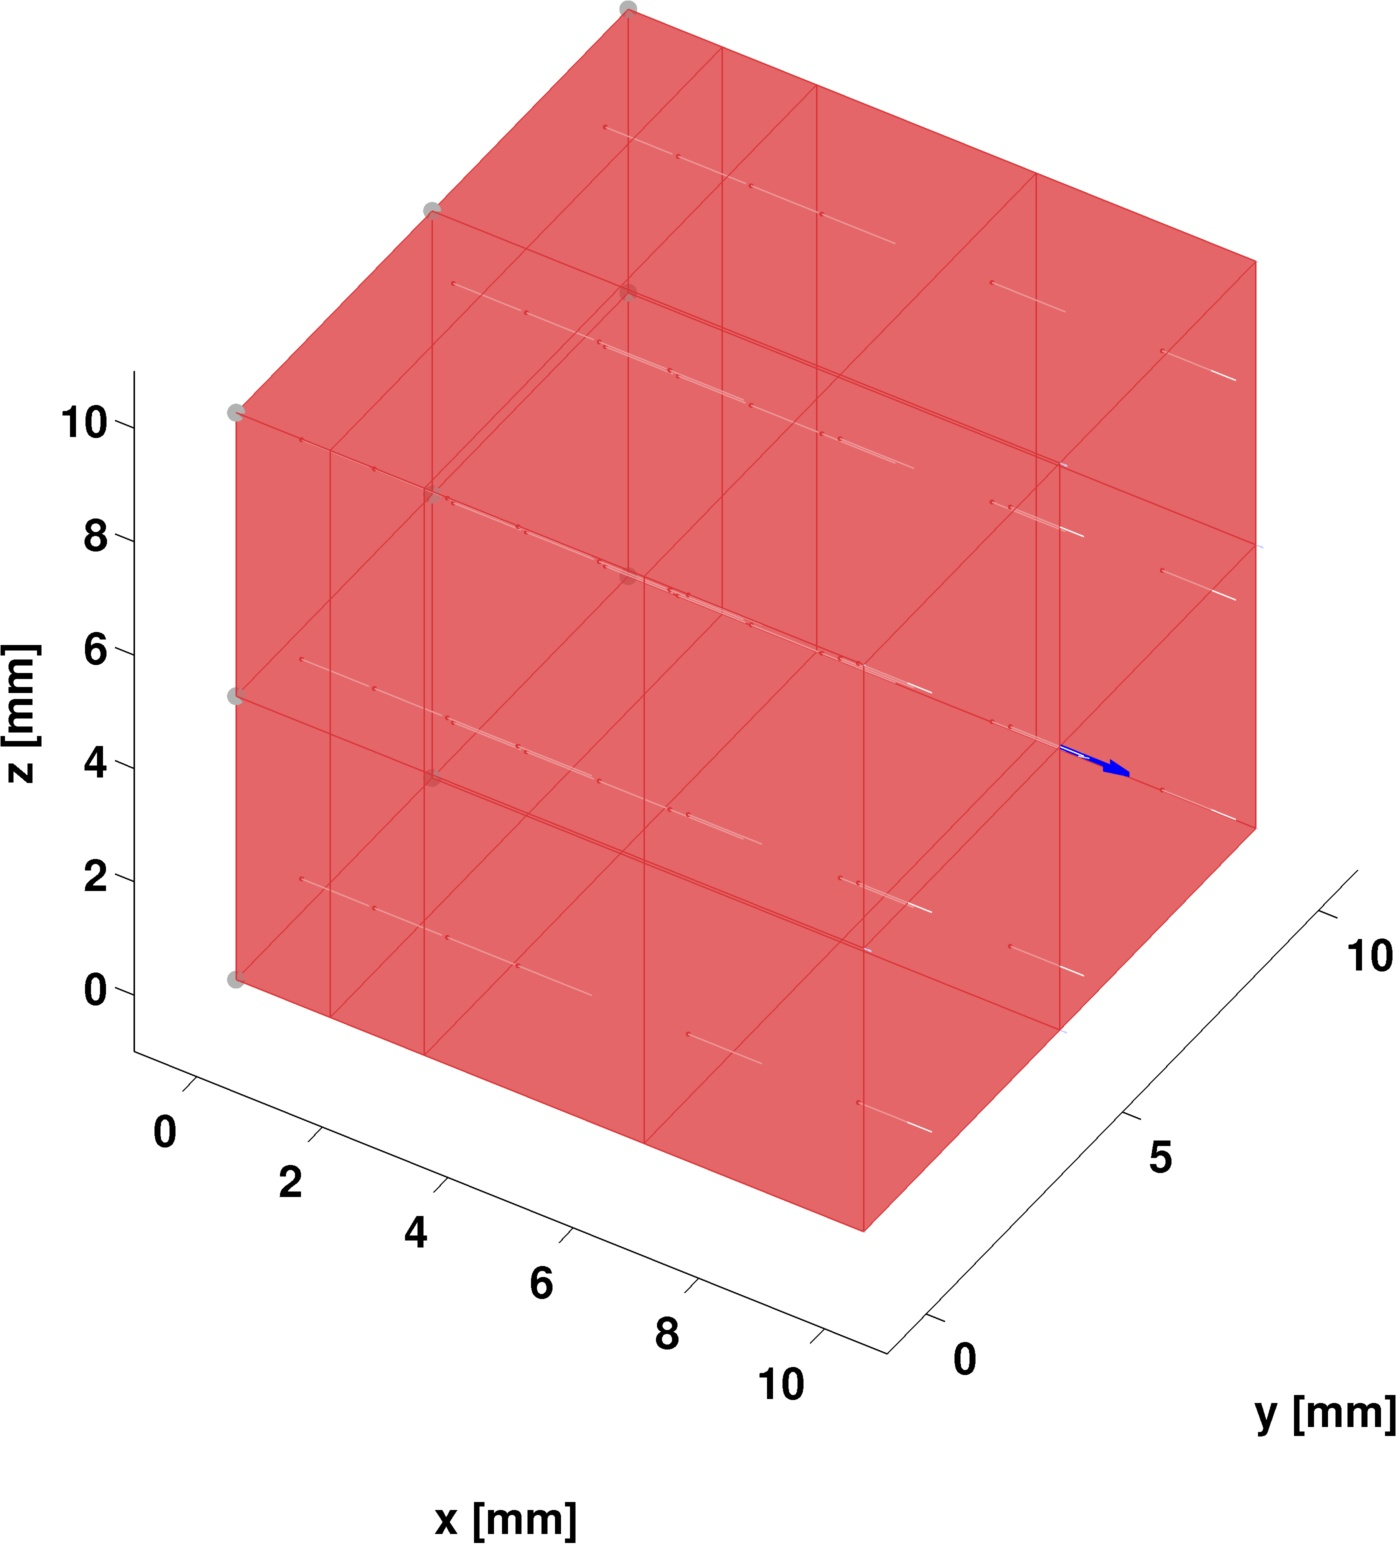
\includegraphics[width=\third]{geo_2_conf_1_gauss_3_geo}
% 	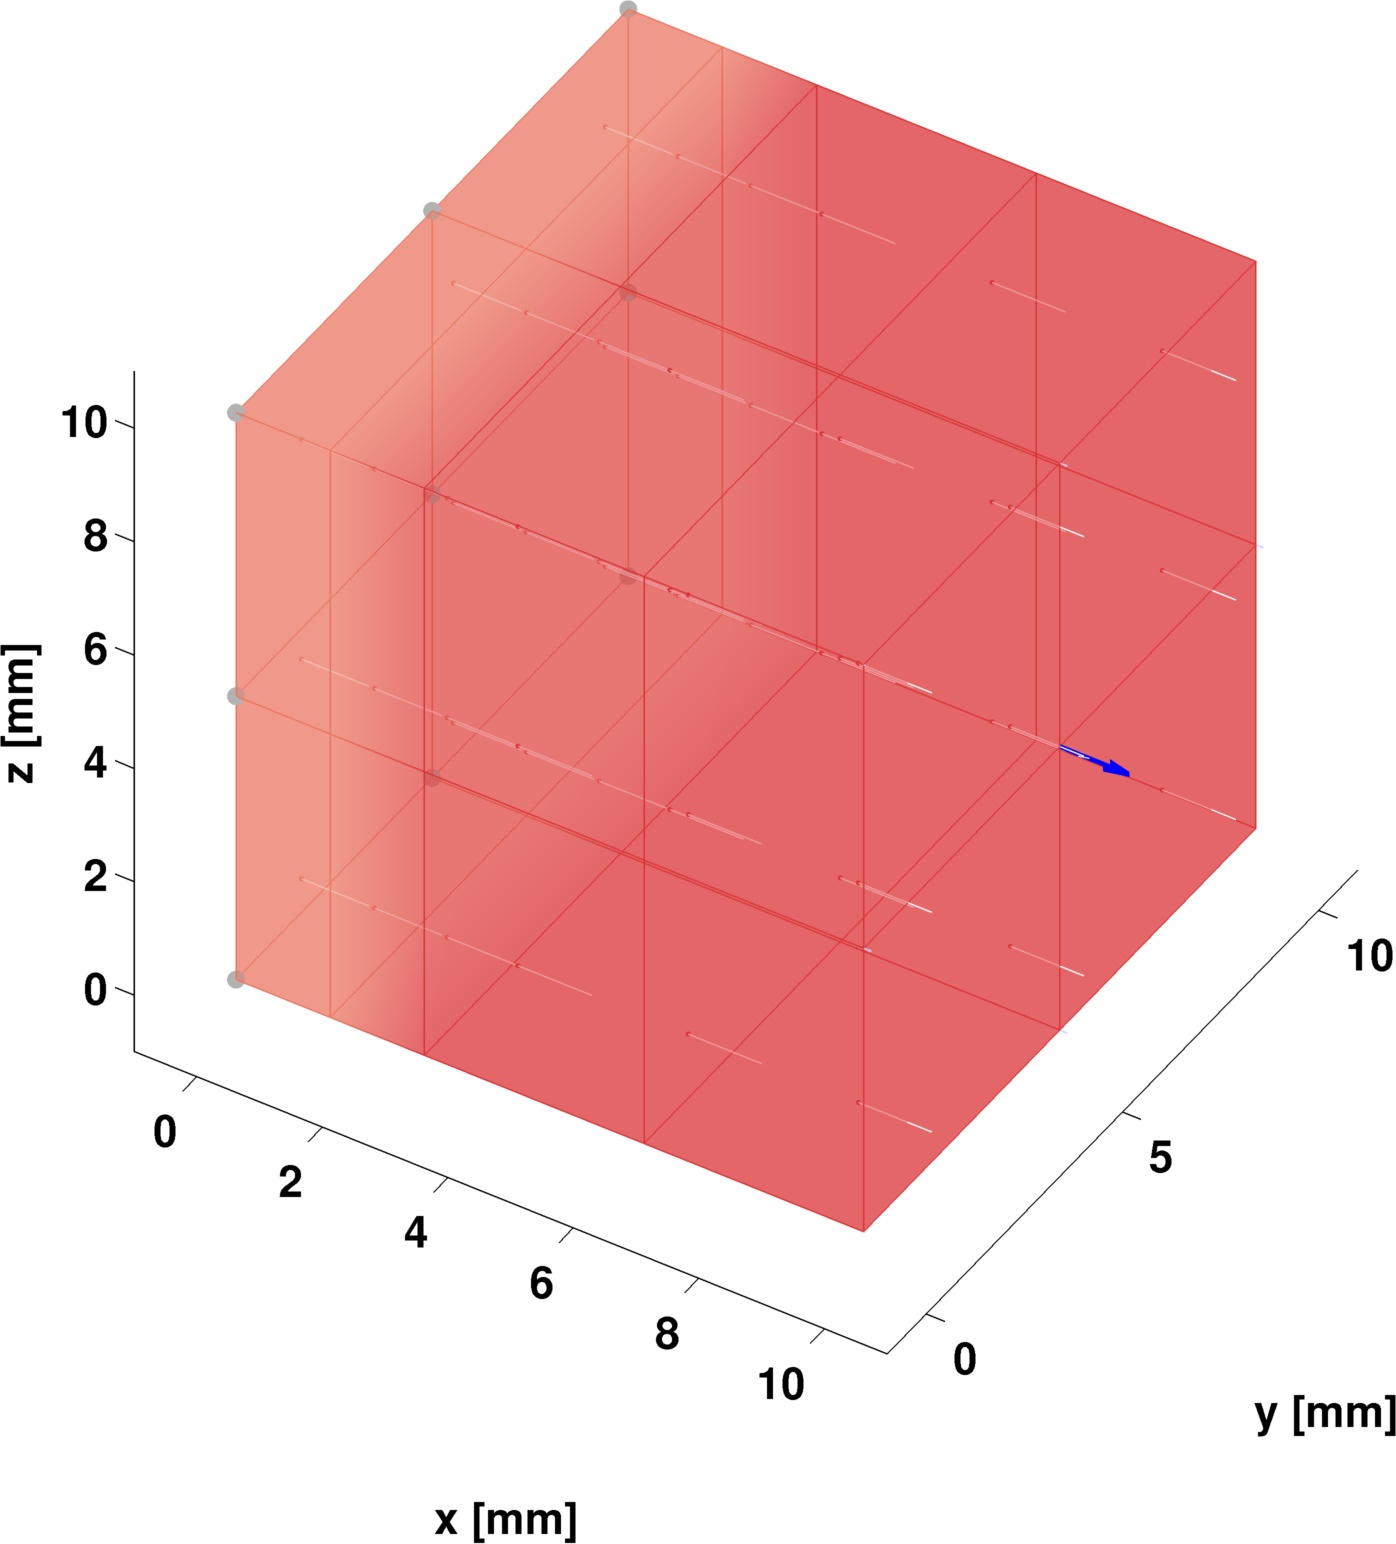
\includegraphics[width=\third]{geo_2_conf_5_gauss_3_geo}
% 	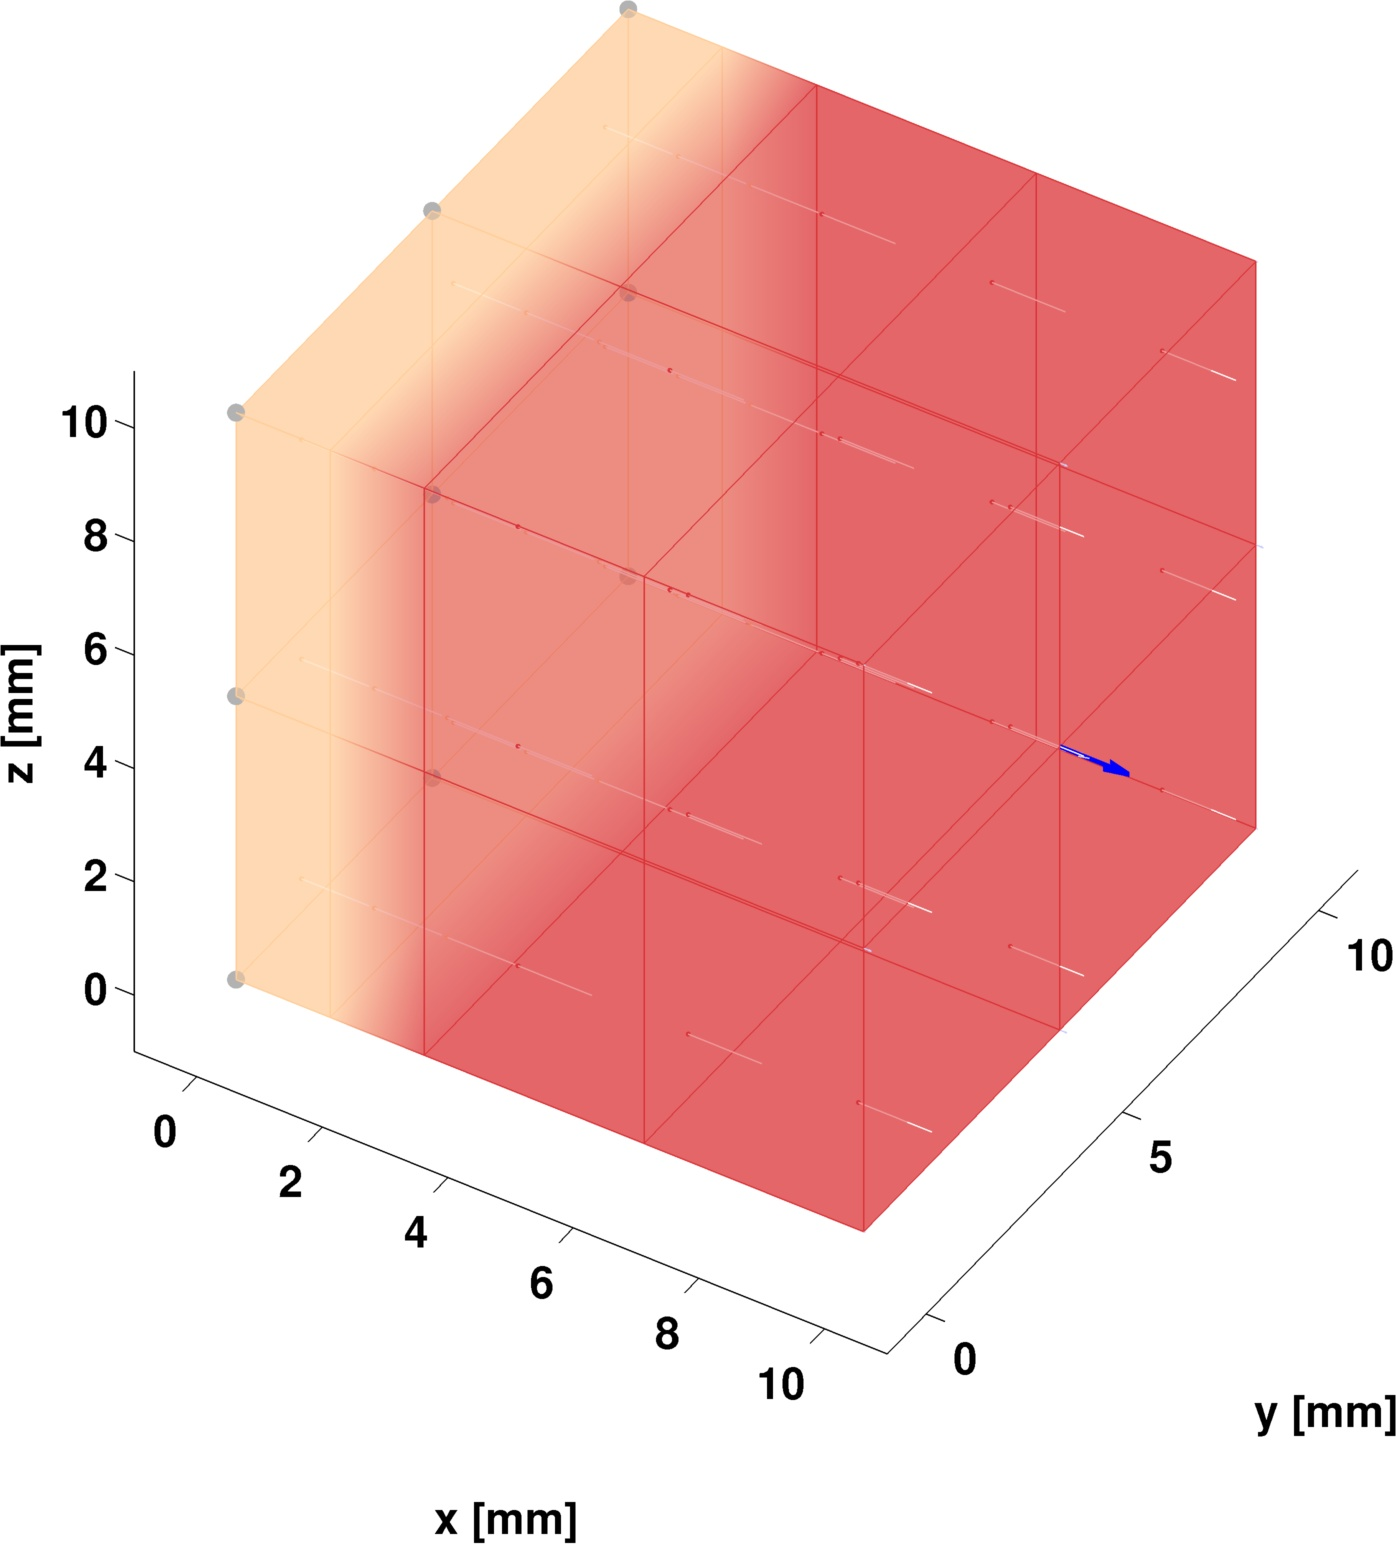
\includegraphics[width=\third]{geo_2_conf_10_gauss_3_geo}\\
% 	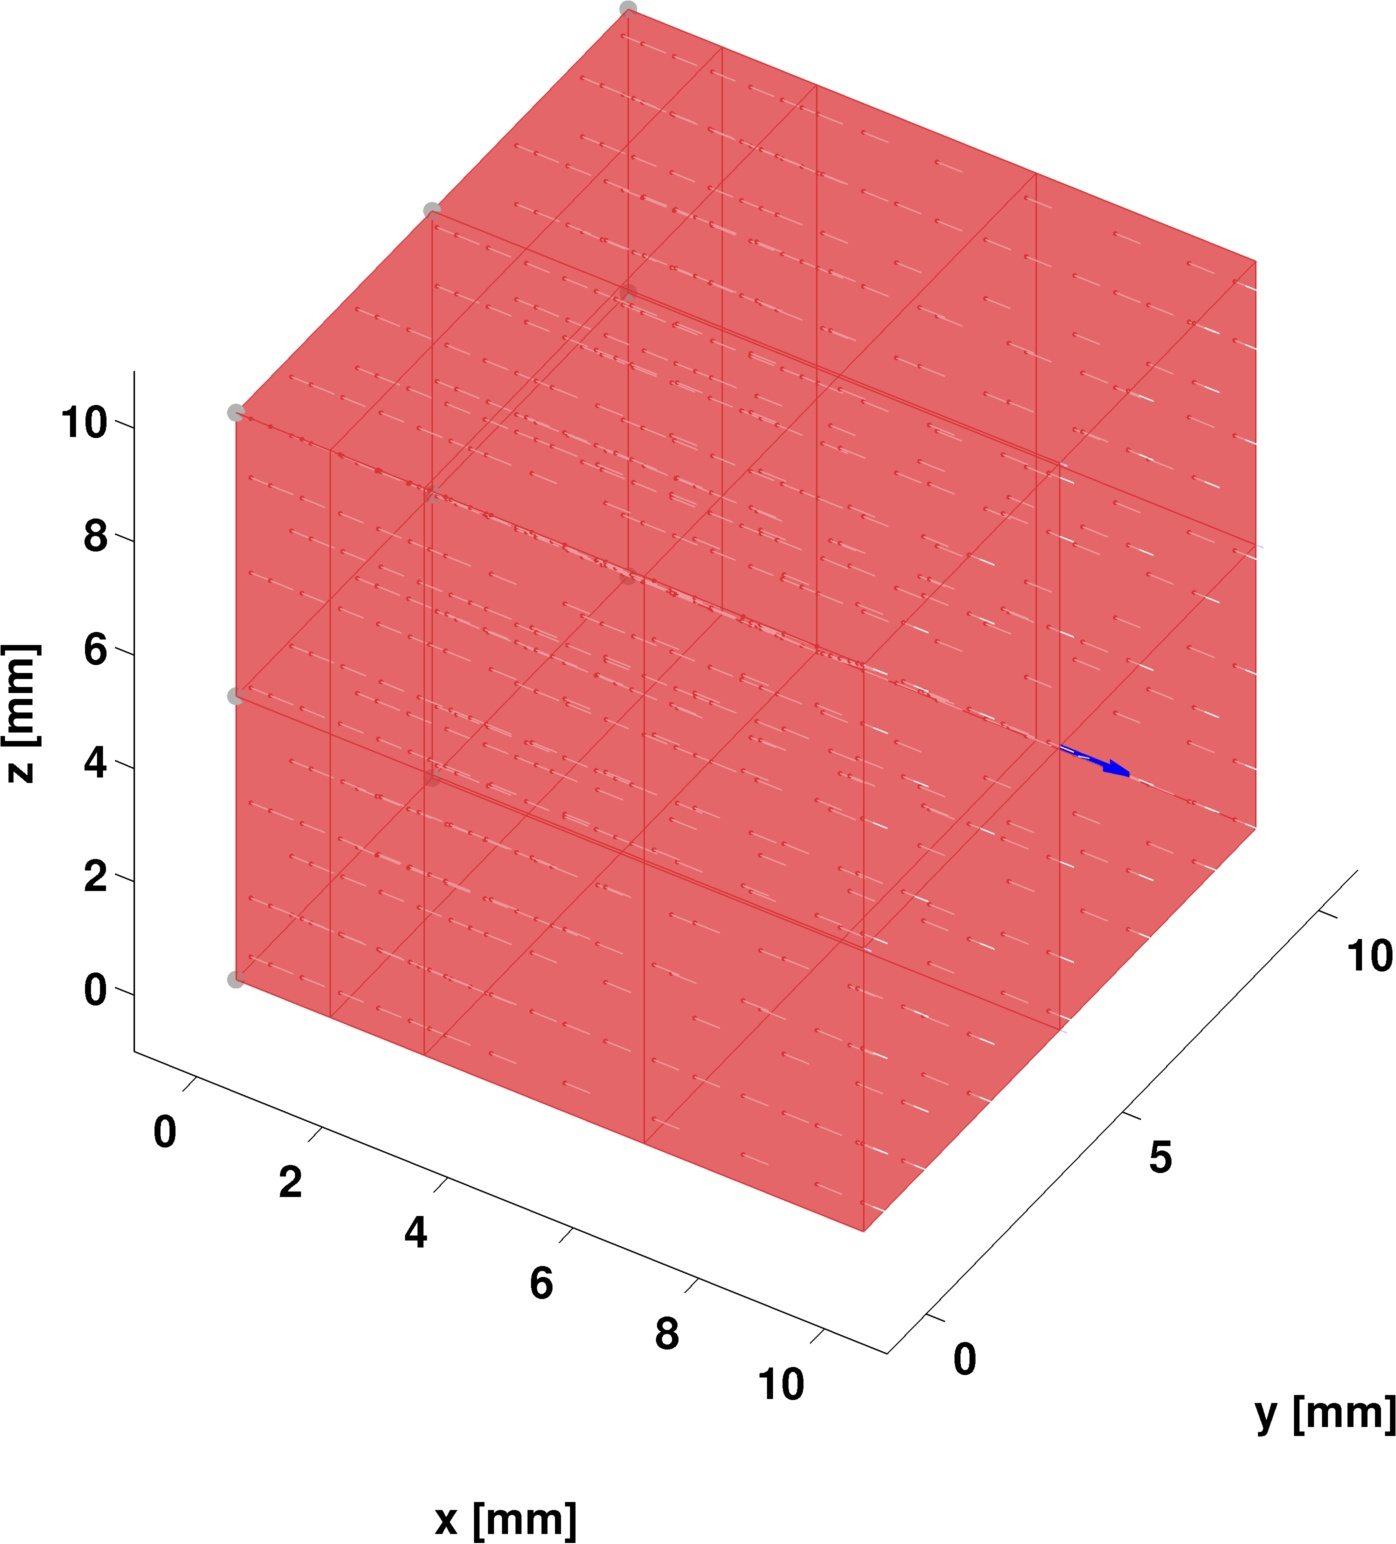
\includegraphics[width=\third]{geo_2_conf_1_gauss_7_geo}
% 	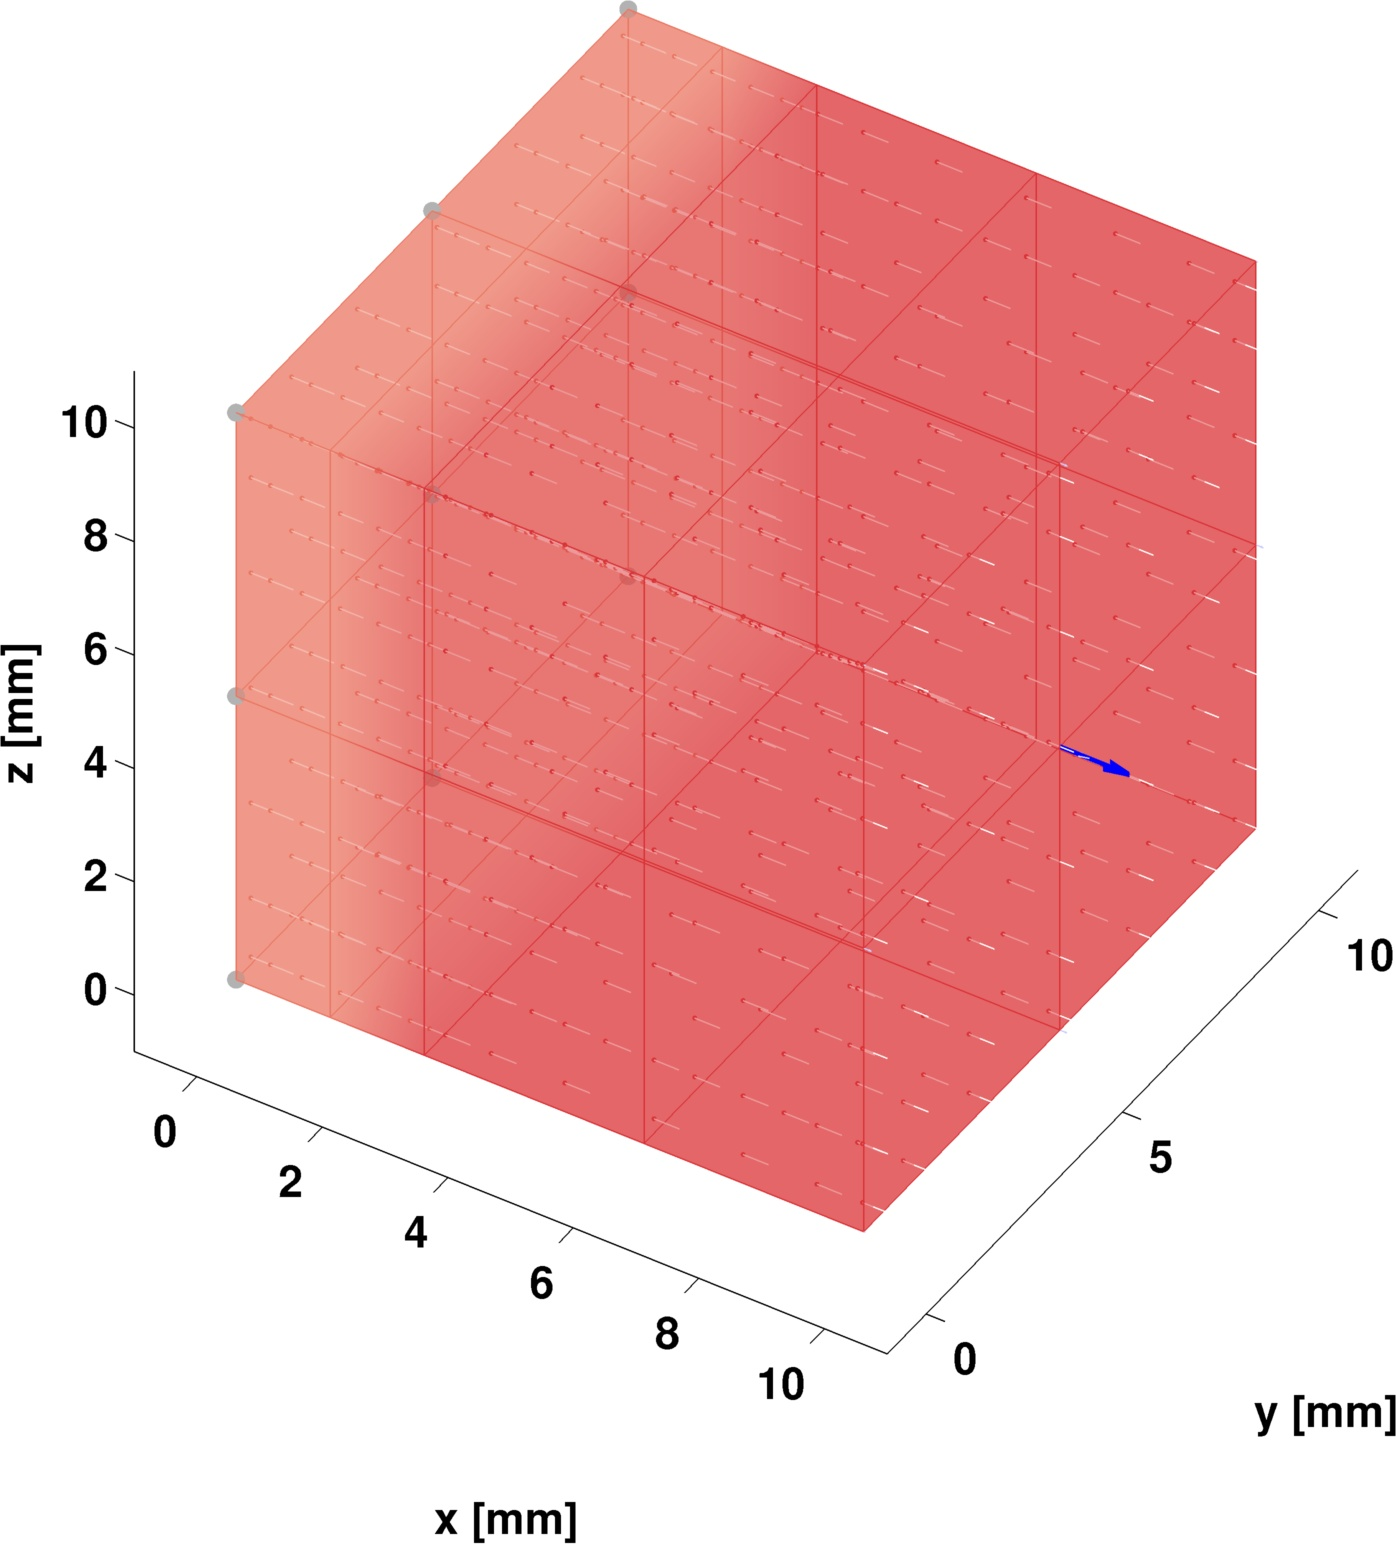
\includegraphics[width=\third]{geo_2_conf_5_gauss_7_geo}
% 	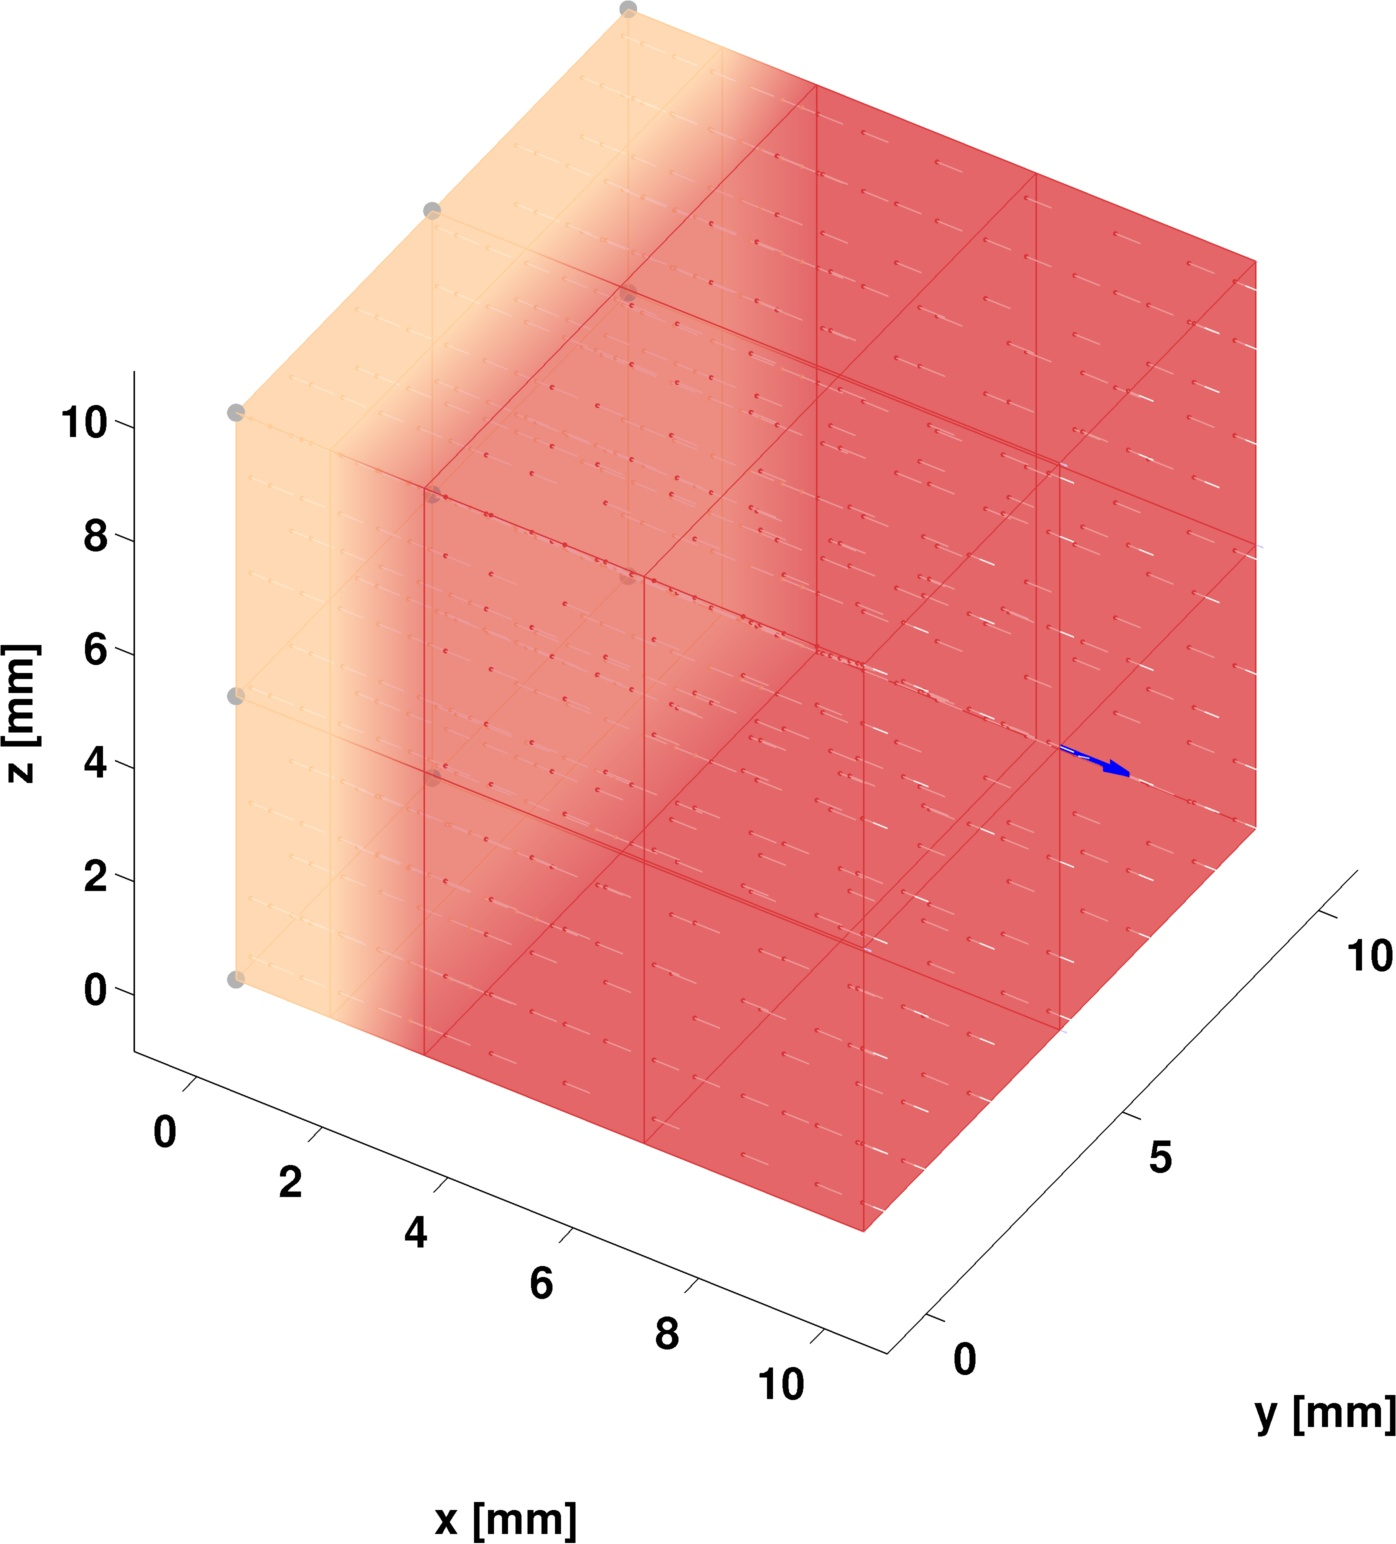
\includegraphics[width=\third]{geo_2_conf_10_gauss_7_geo}\\
% 	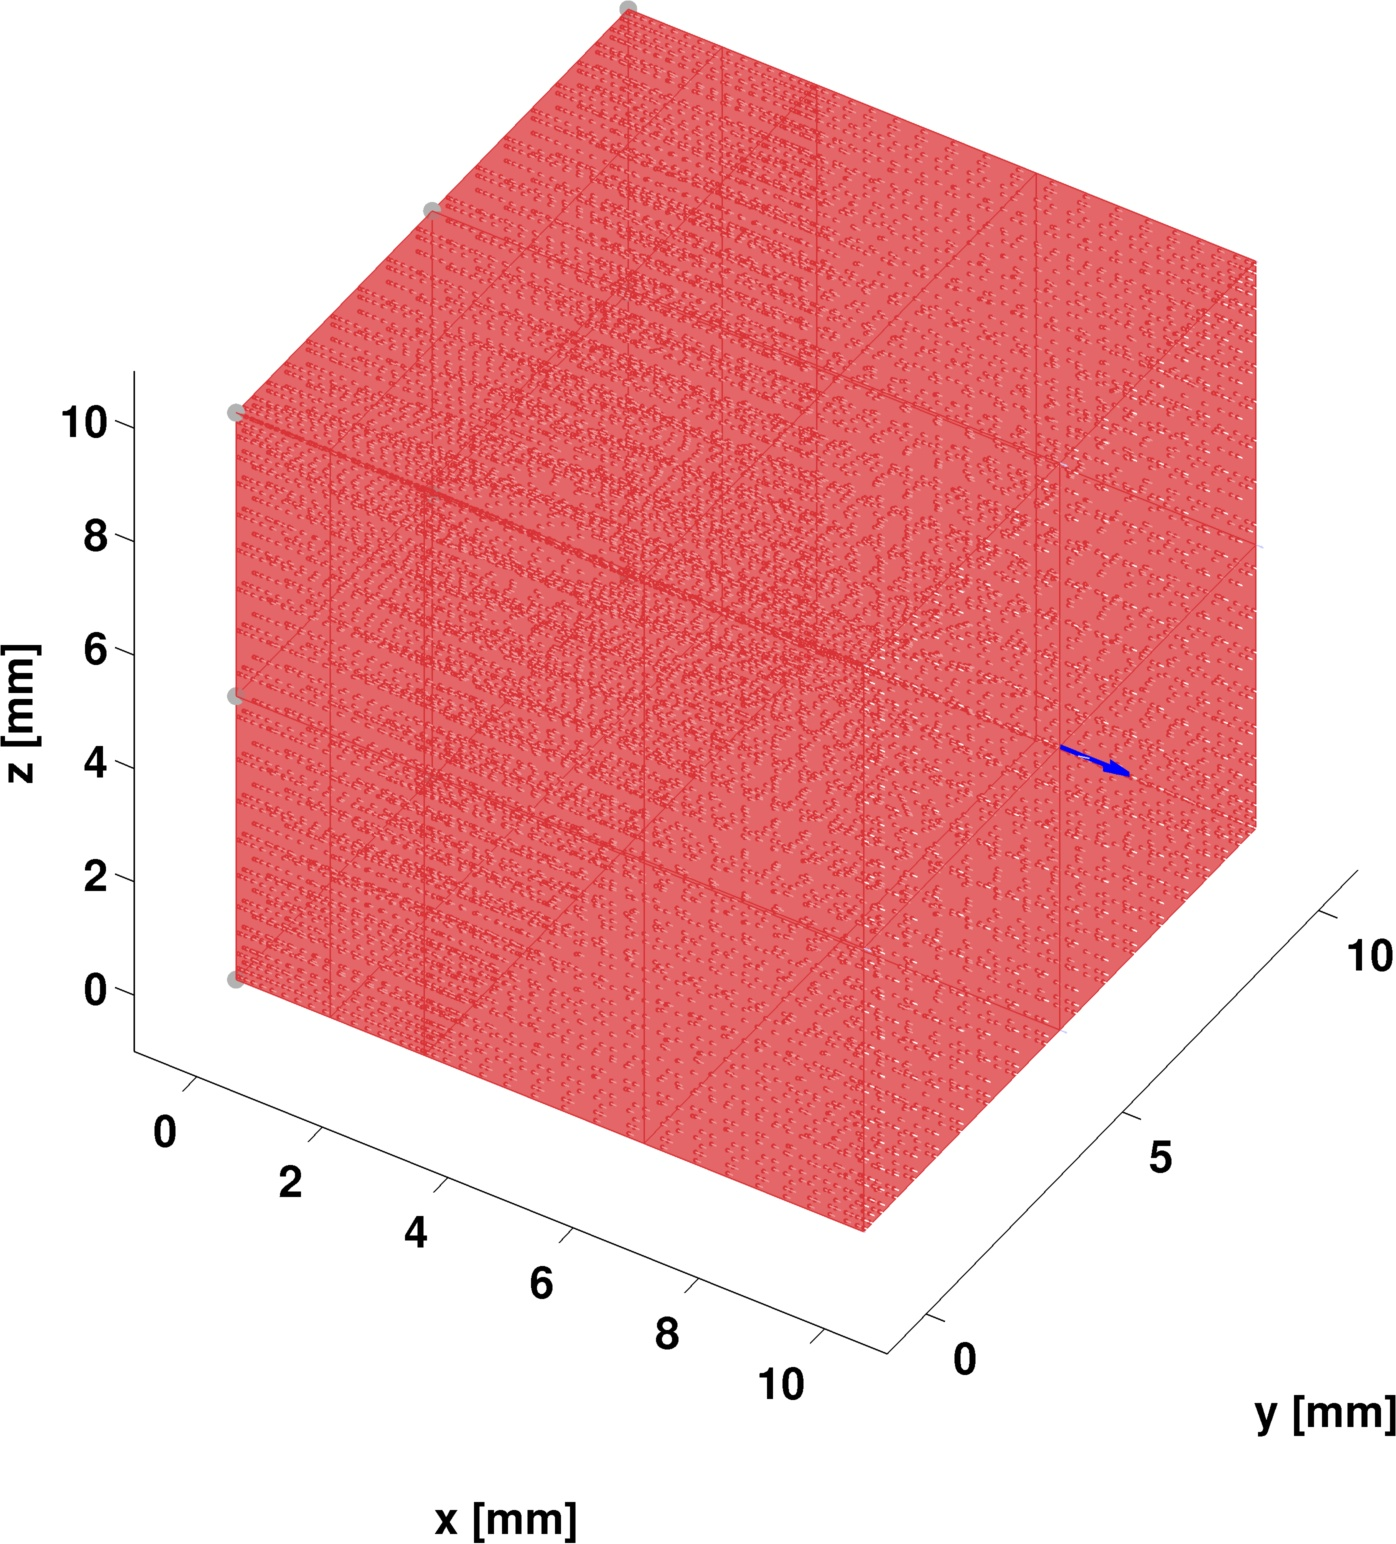
\includegraphics[width=\third]{geo_2_conf_1_gauss_20_geo}
% 	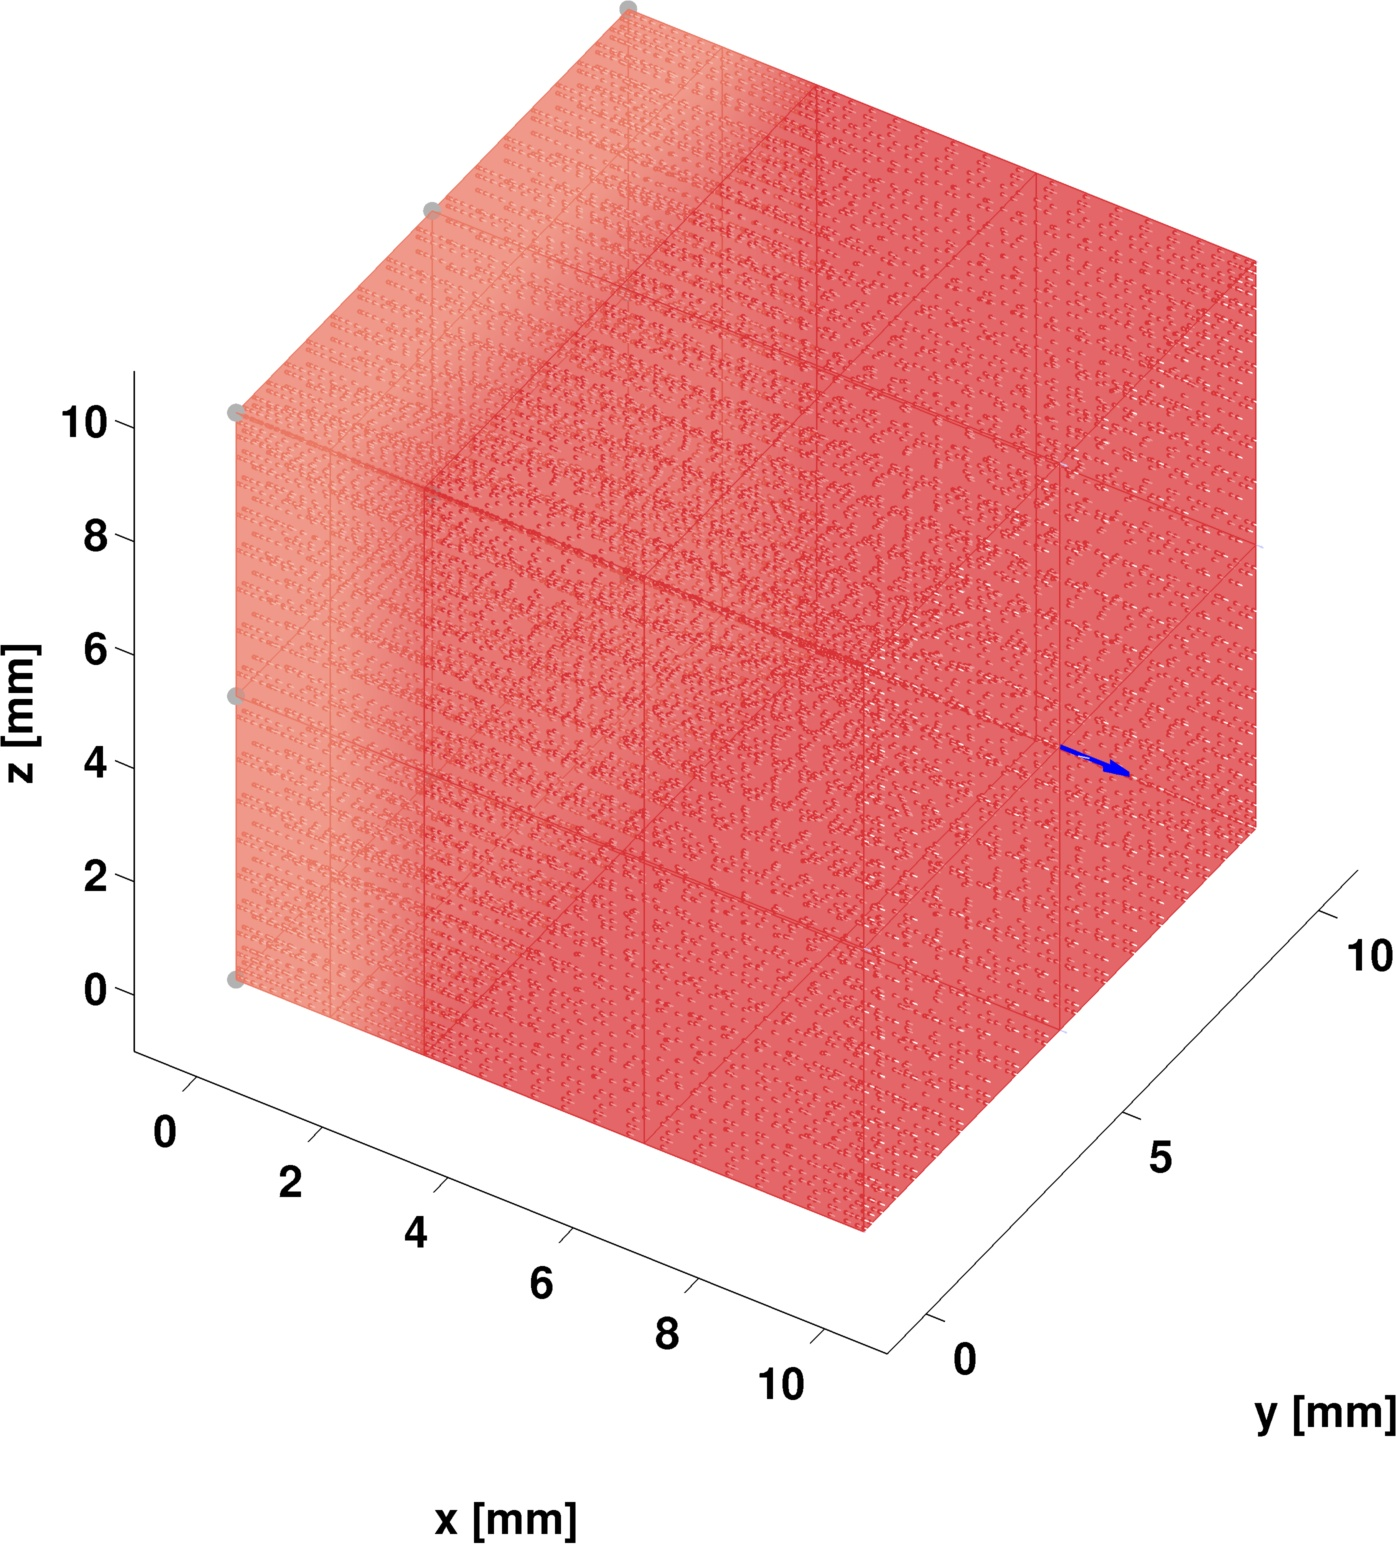
\includegraphics[width=\third]{geo_2_conf_5_gauss_20_geo}
% 	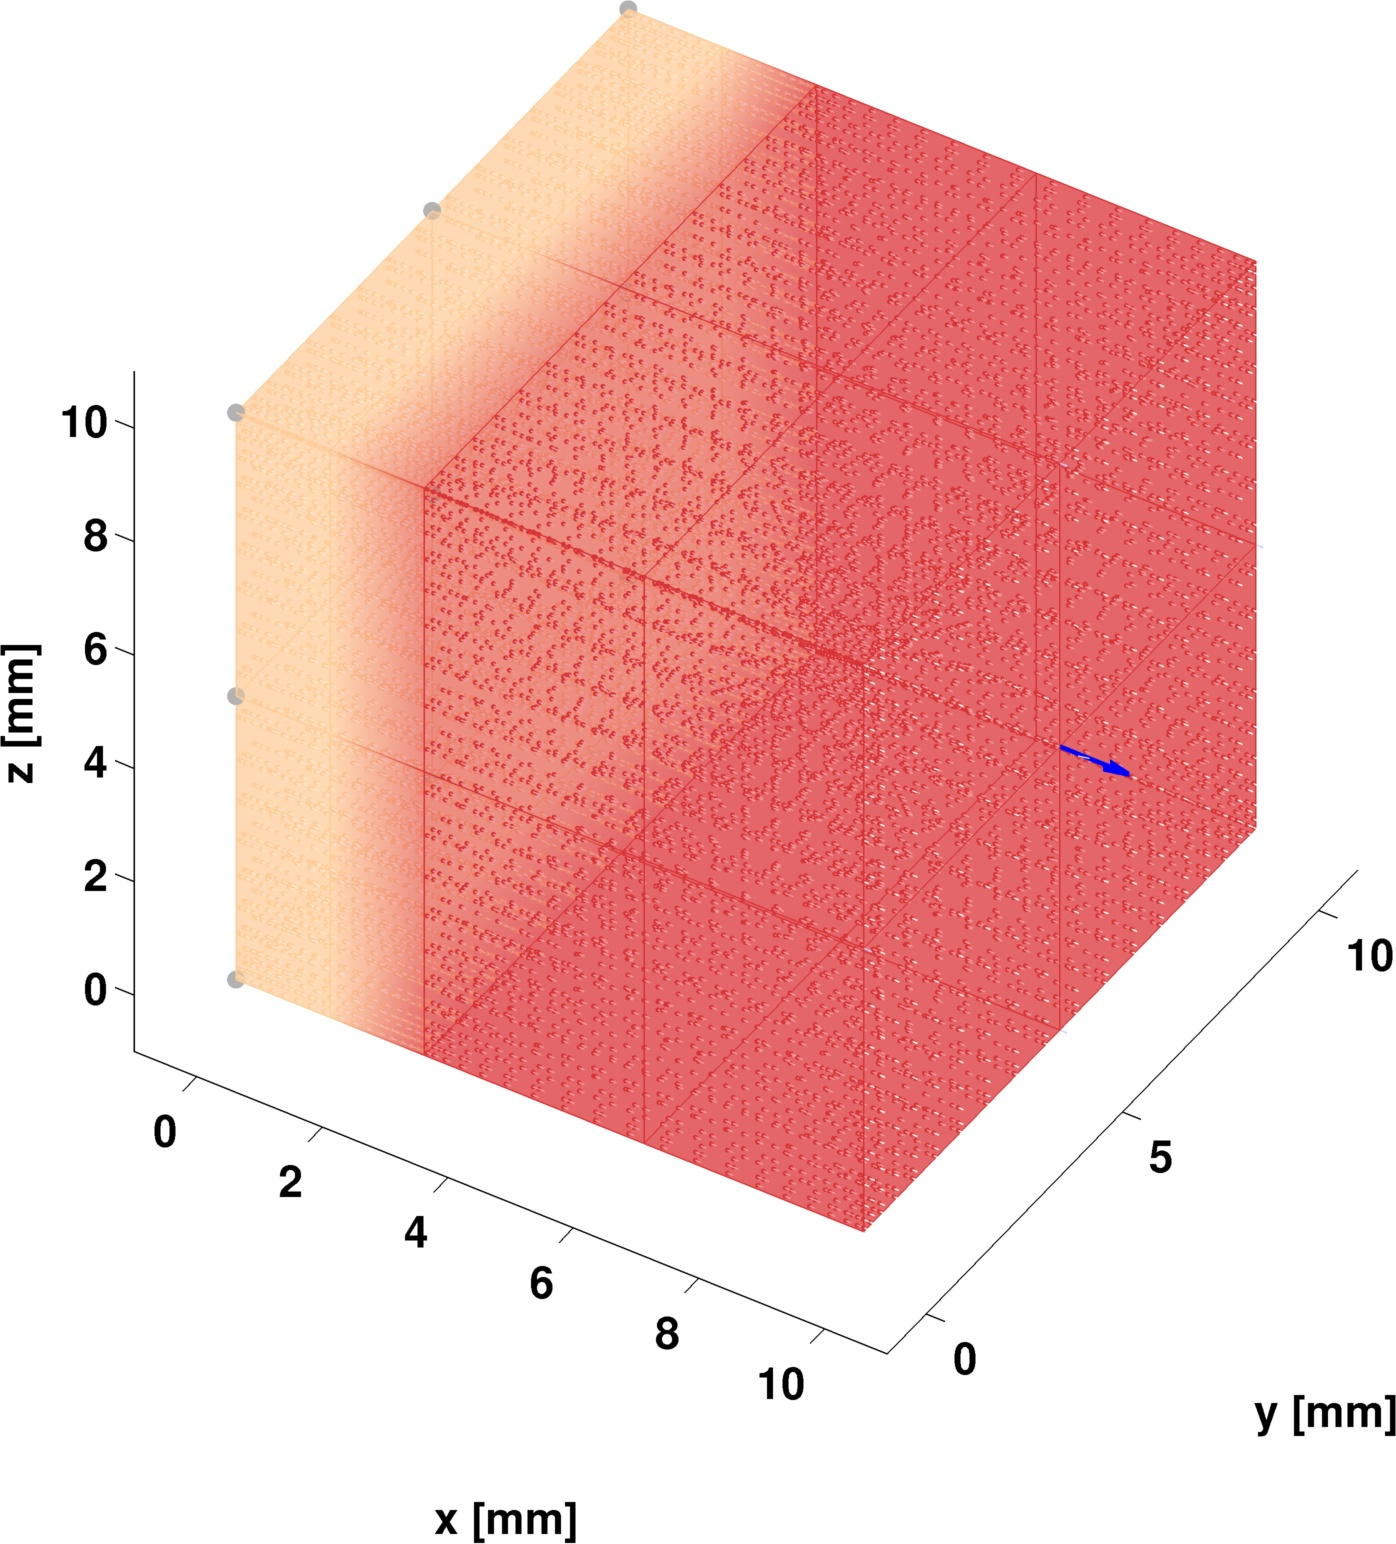
\includegraphics[width=\third]{geo_2_conf_10_gauss_20_geo}\\
	\caption{Experiment geometry for case 2: two elements split at $3$.
	Left to right: configurations $\theta_1,\theta_5,\theta_{10}$, top to bottom: gauss integration rules $3,7,20$ points}
	\label{fig:geo2}
\end{figure}

%%%%%%%%%%%%%%%%%%%%%%%%%%%%%%%%%%% RESULTS %%%%%%%%%%%%%%%%%%%%%%%%%%%%%%%%%%%
%%%%%%%%%%%%%%%%%%%%%%%%%%%%%%%%%%%%%%%%%%%%%%%%%%%%%%%%%%%%%%%%%%%%%%%%%%%%%%% 
\subsection{Results}
\subsubsection{One element case}
\begin{figure}[!ht]
	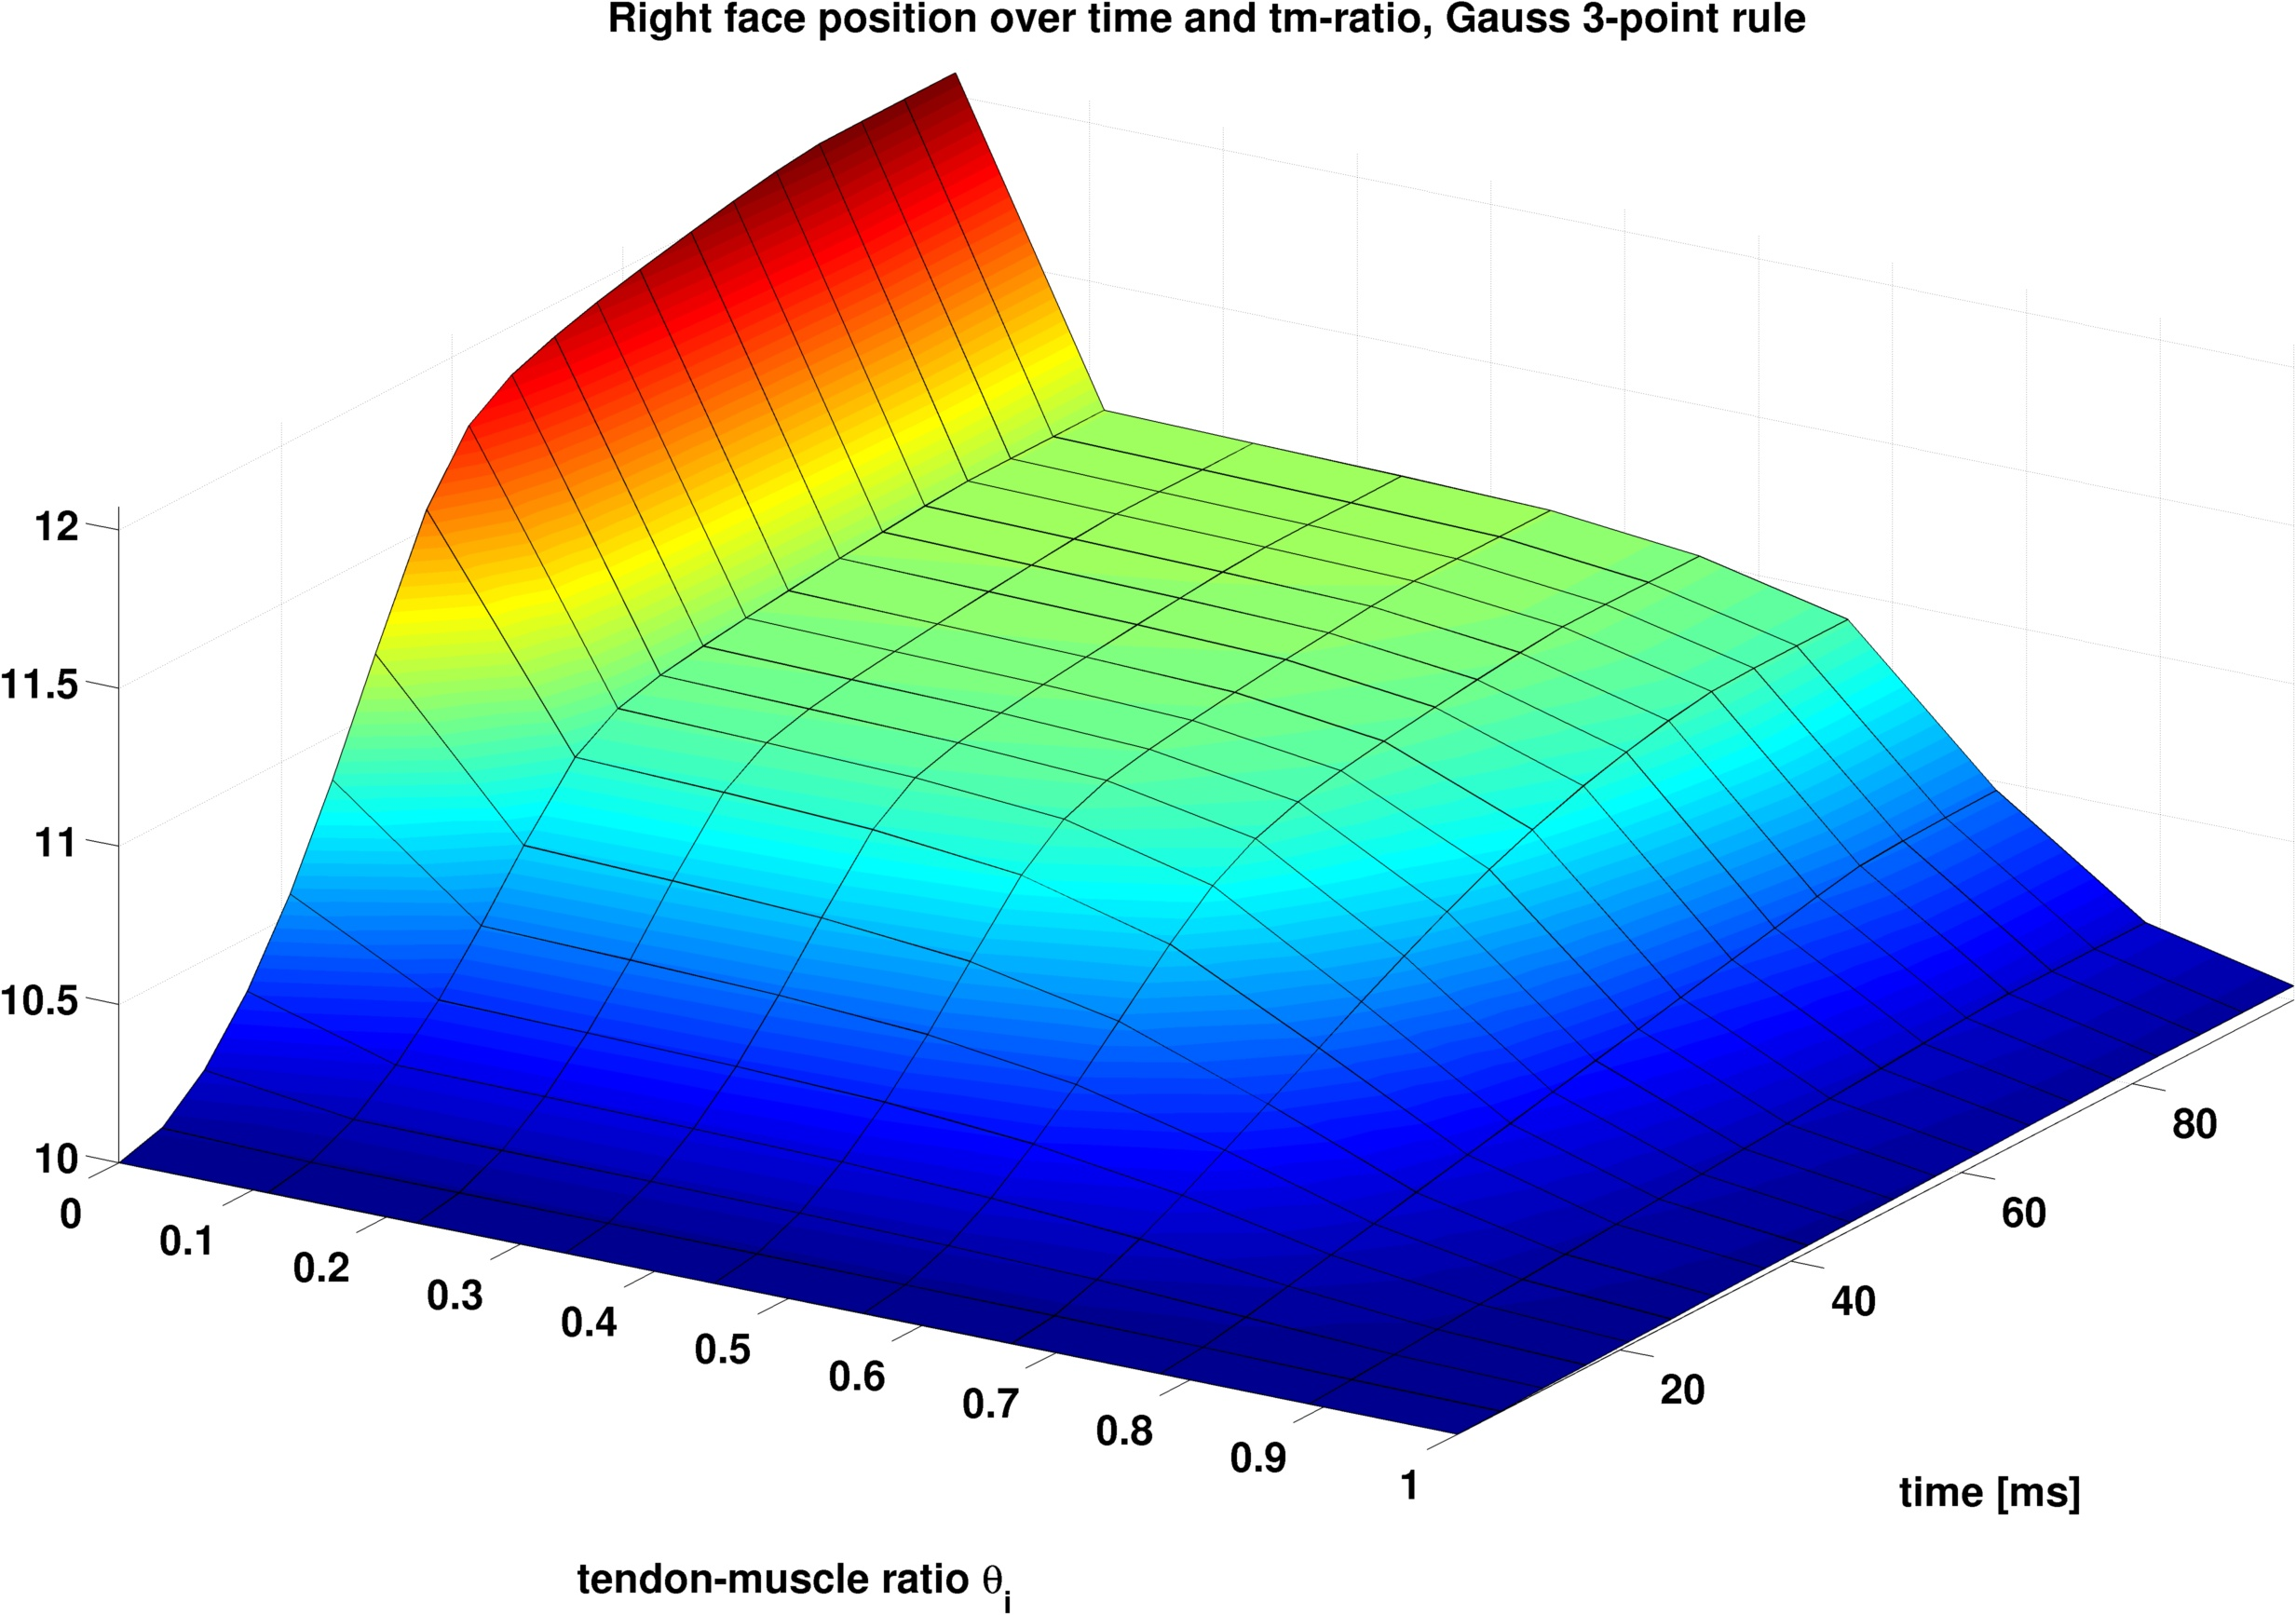
\includegraphics[width=\half]{geo_1_gaussrule_3}
% 	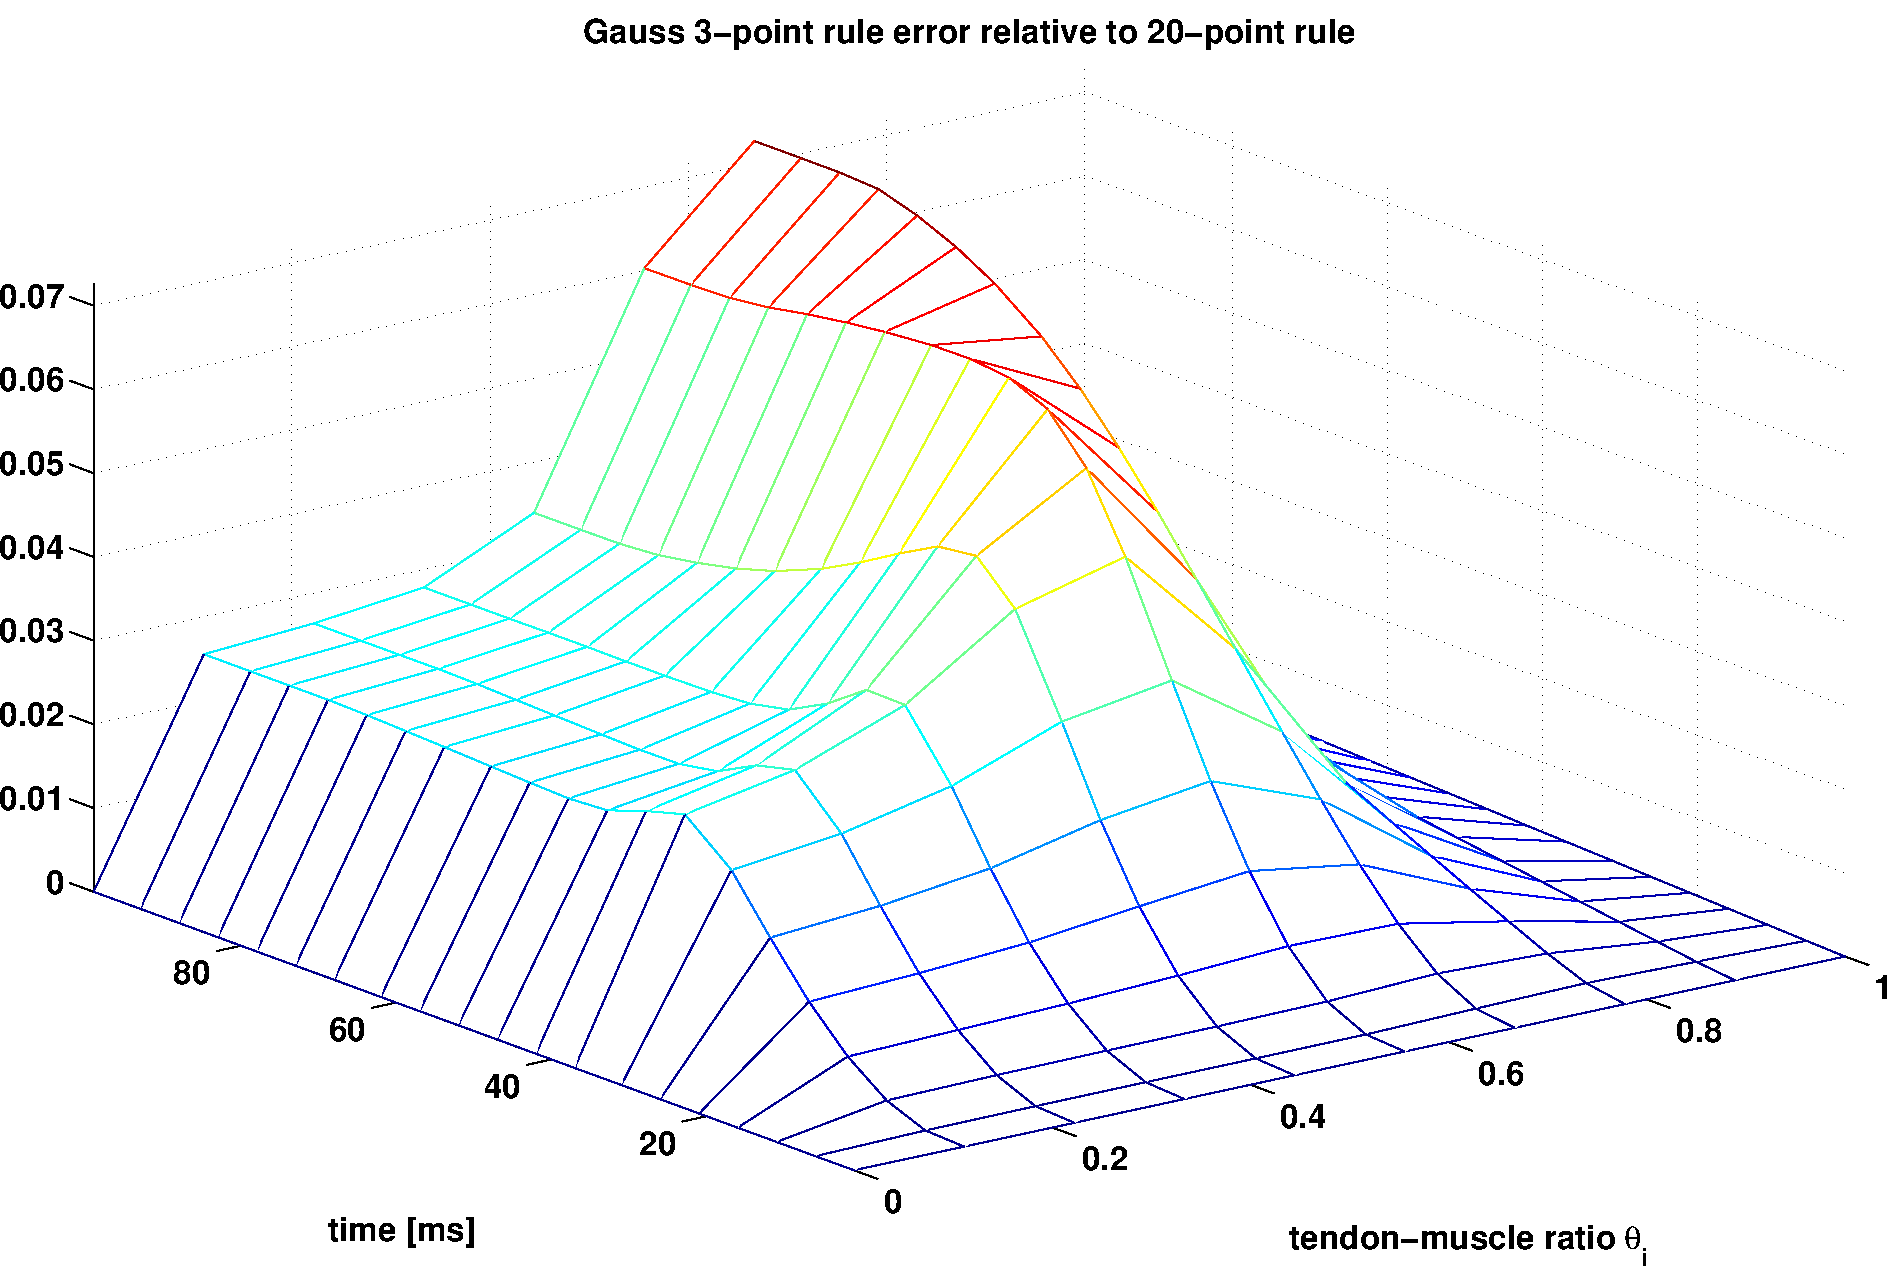
\includegraphics[width=\half]{geo_1_gaussrule_3_err}\\
% 	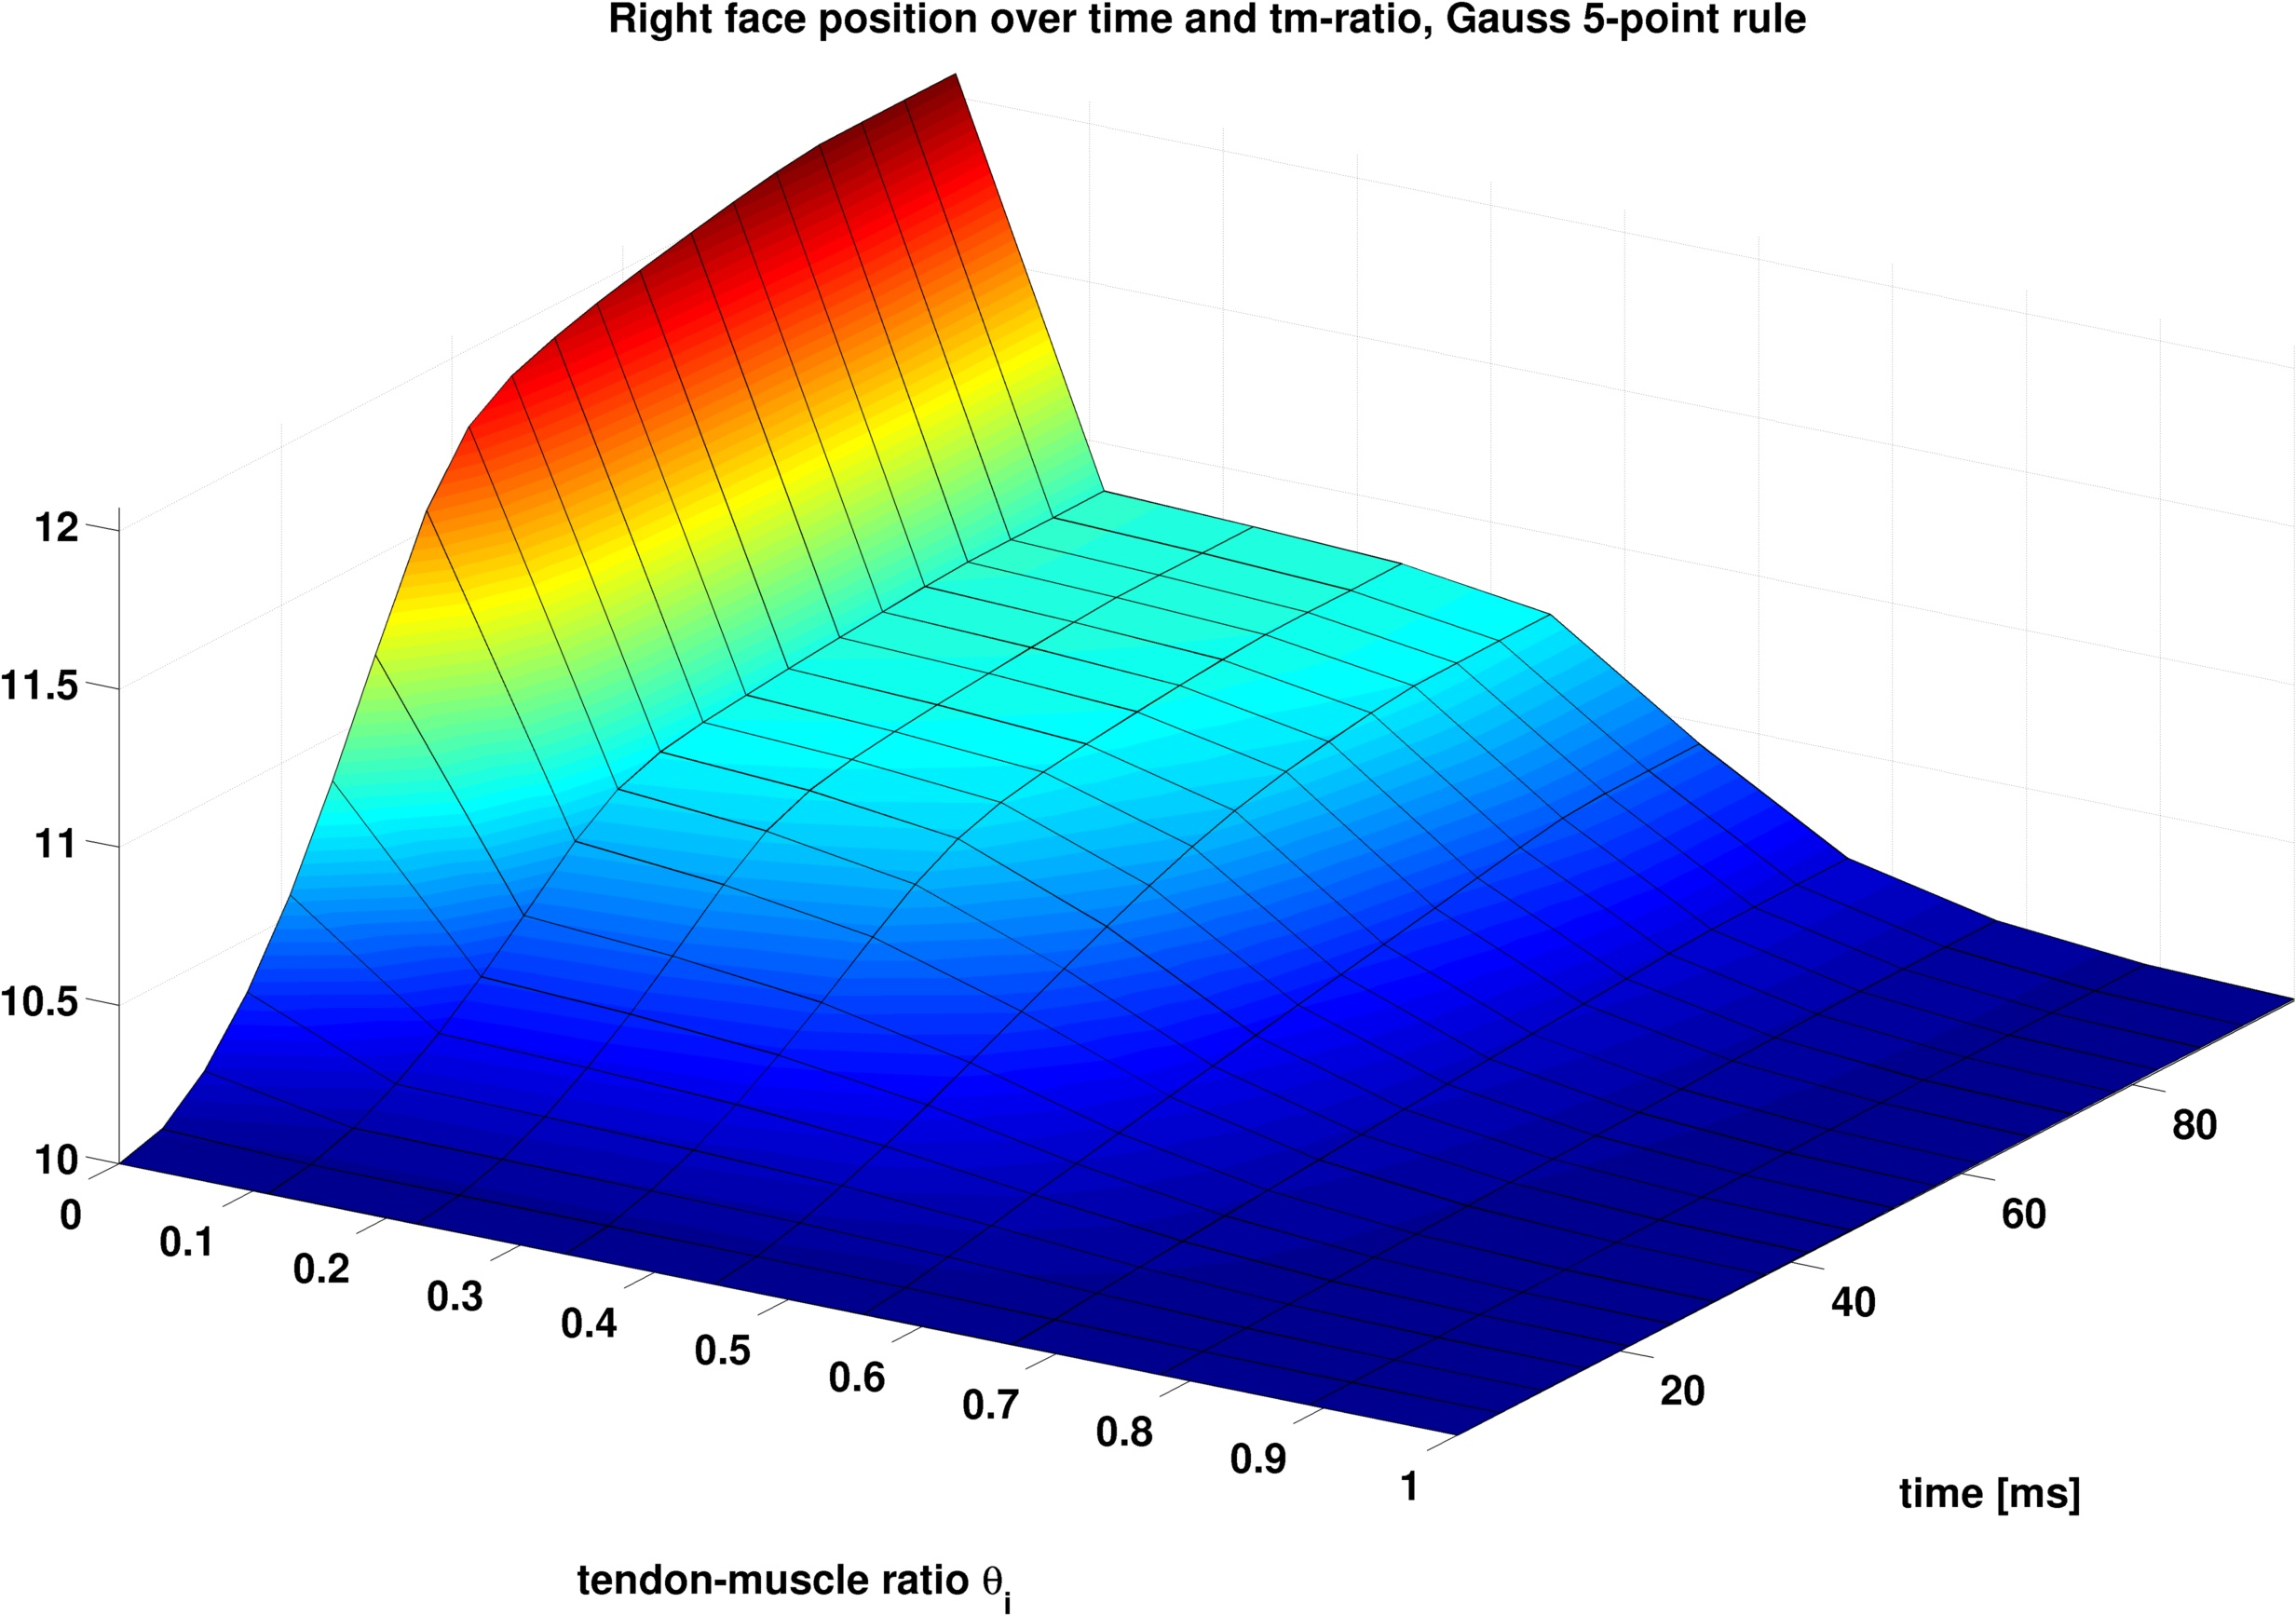
\includegraphics[width=\half]{geo_1_gaussrule_5}
% 	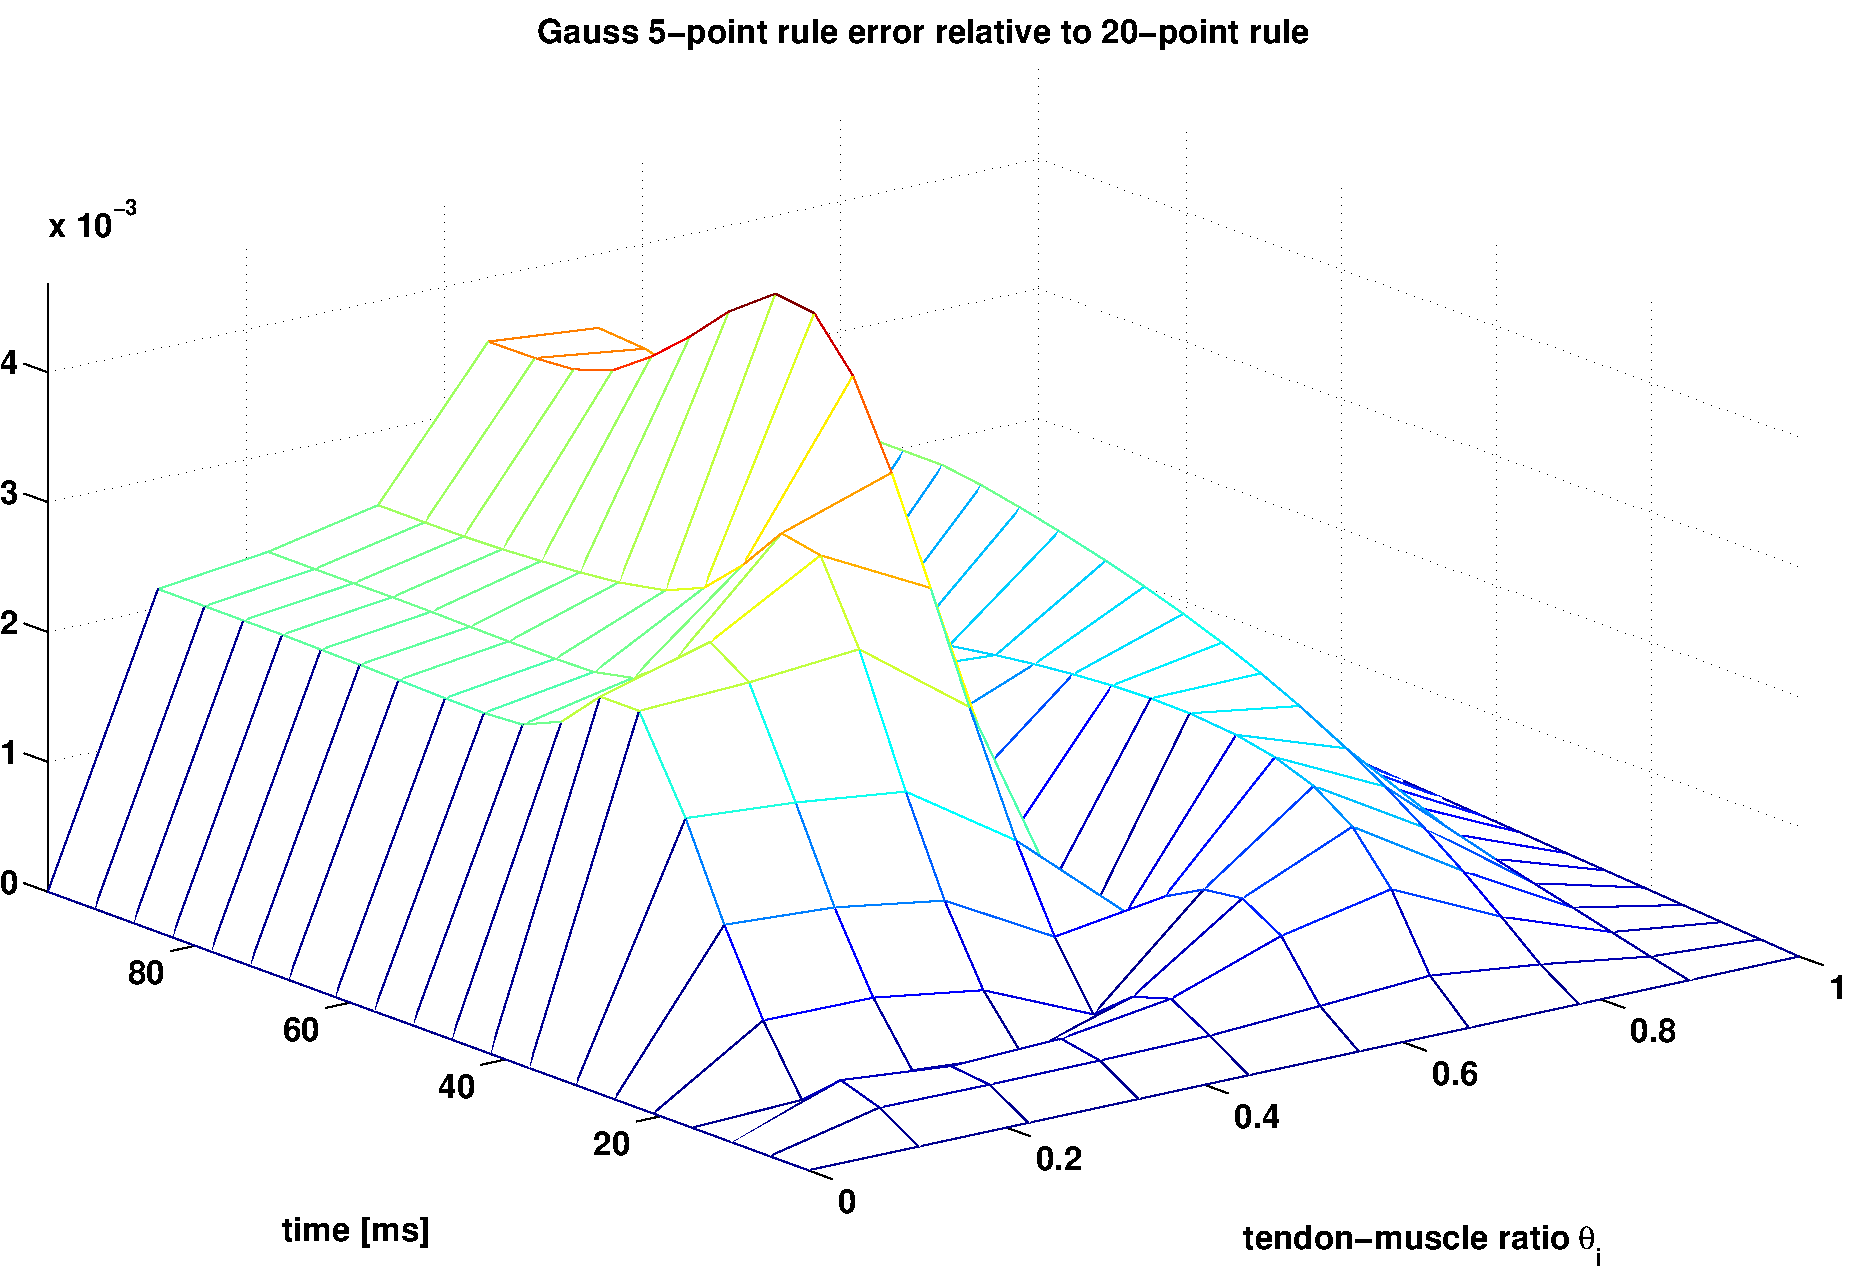
\includegraphics[width=\half]{geo_1_gaussrule_5_err}\\
% 	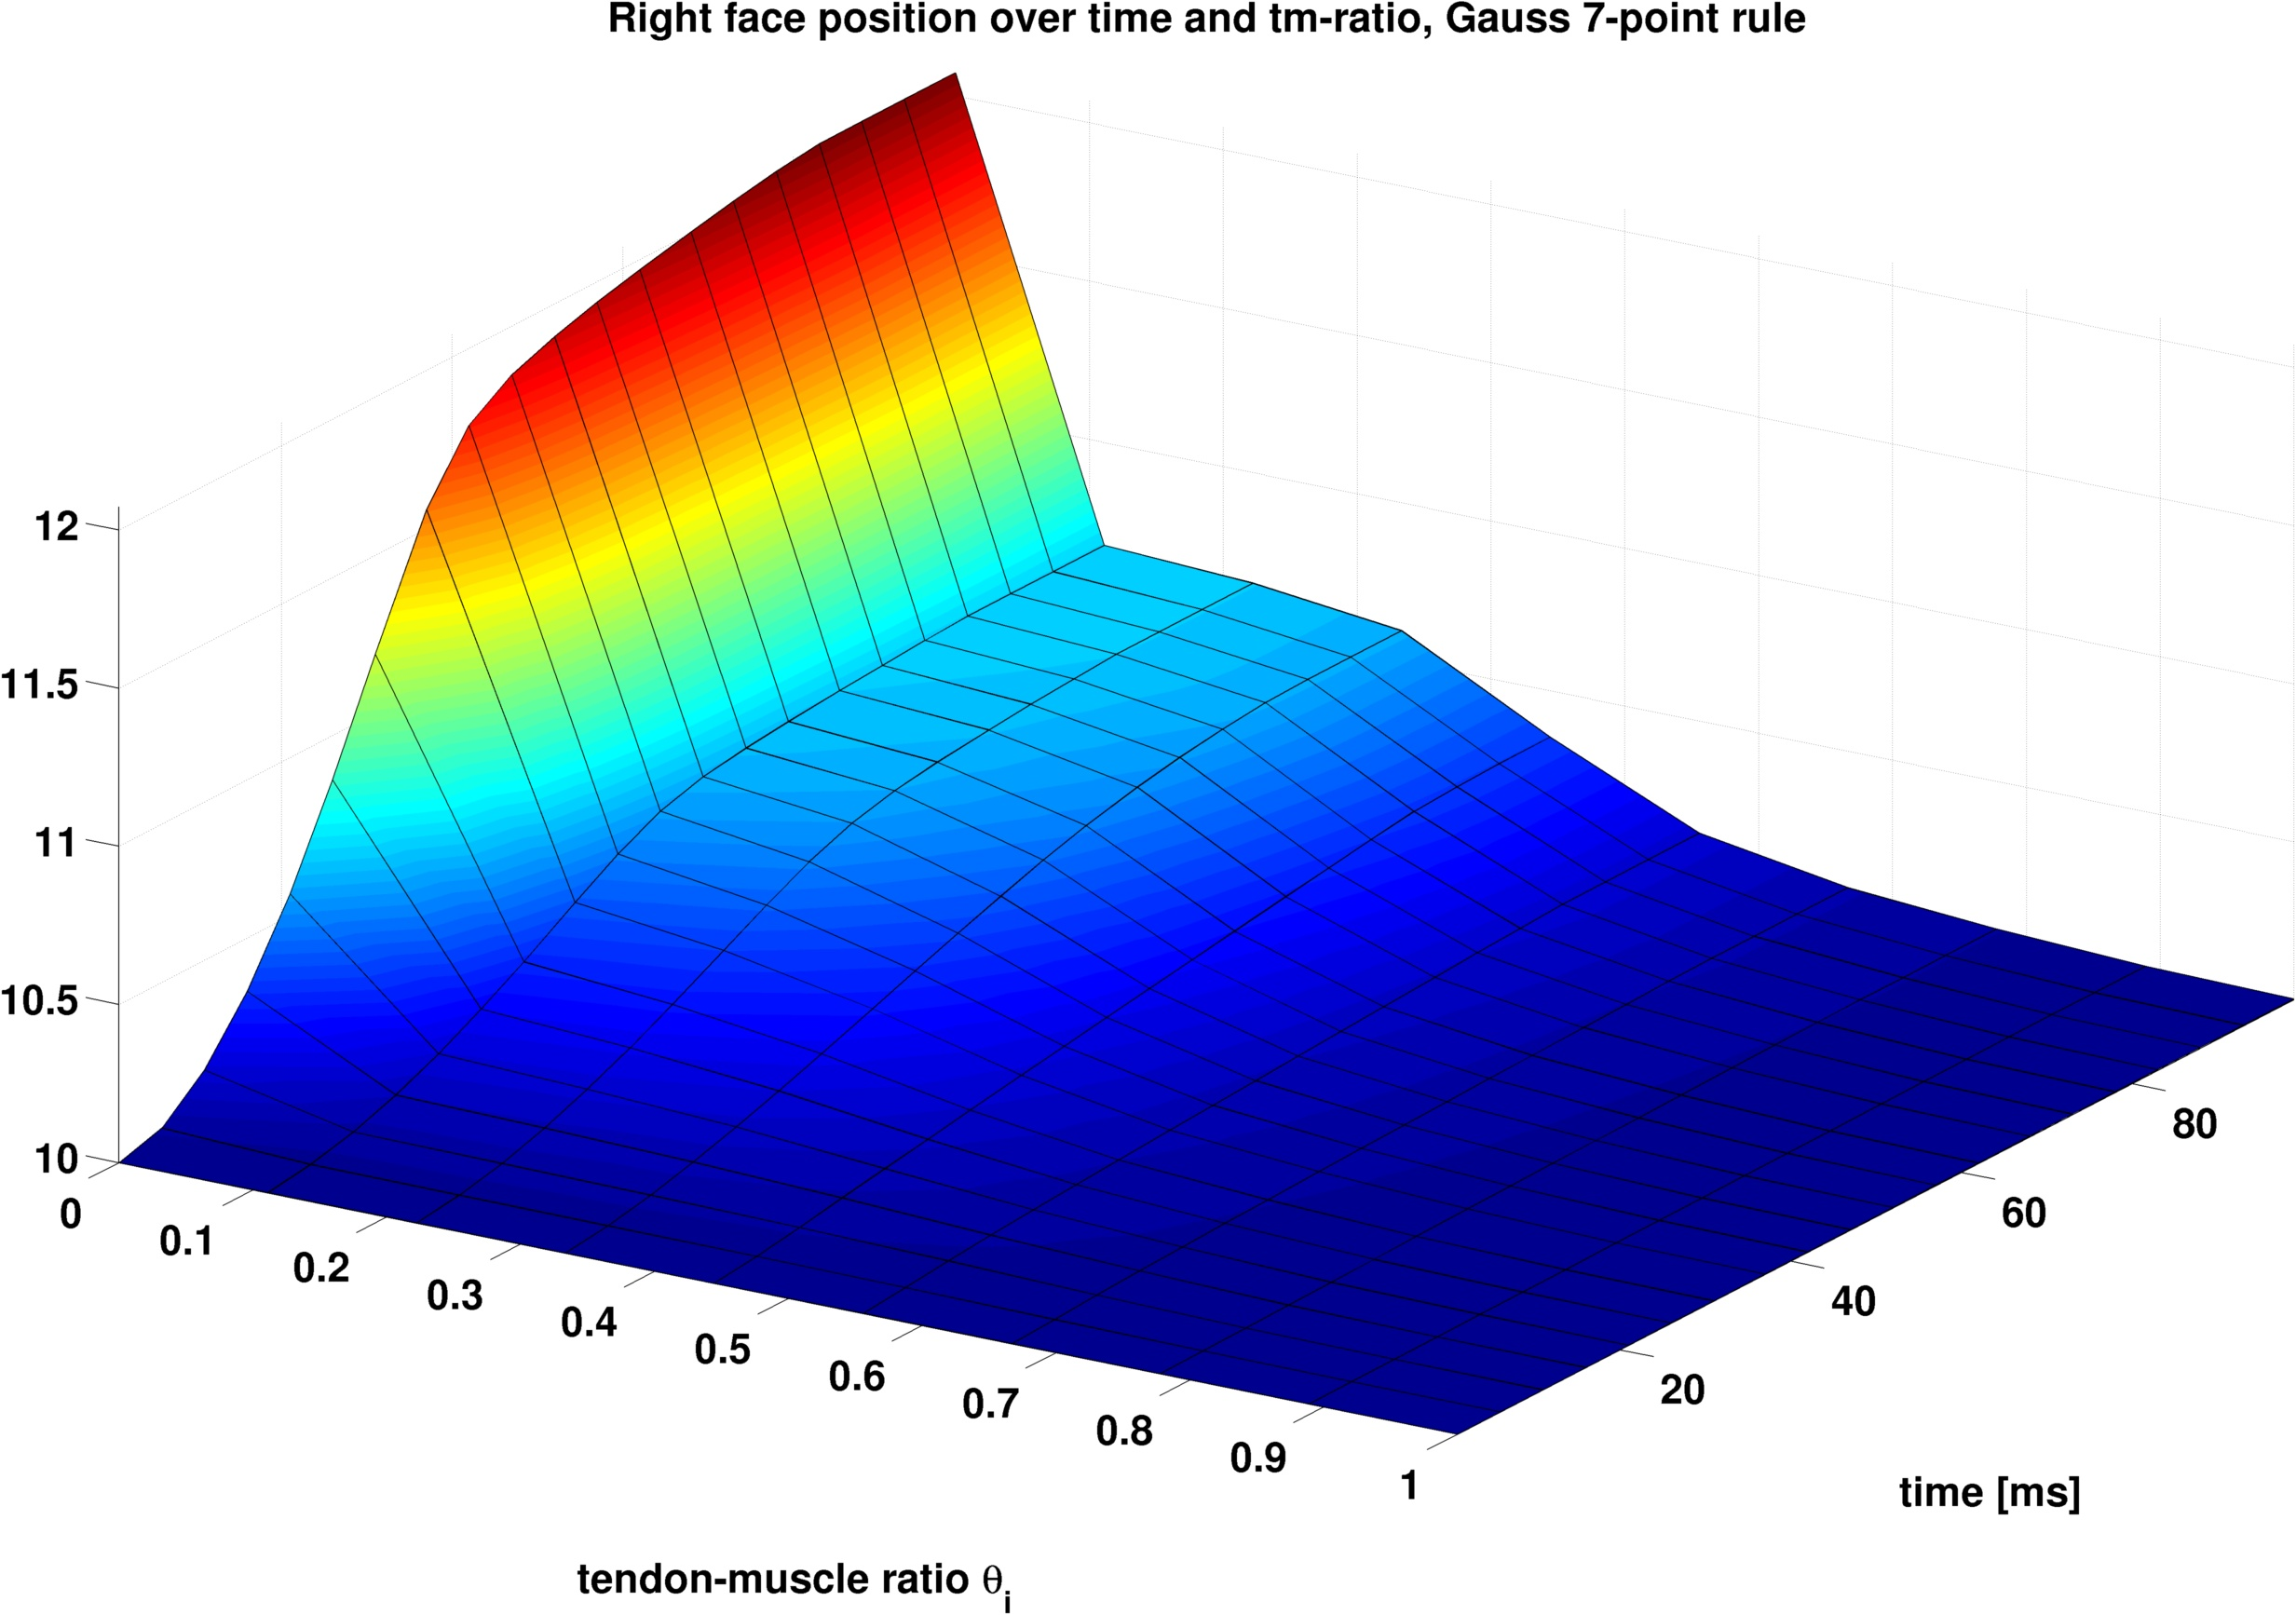
\includegraphics[width=\half]{geo_1_gaussrule_7}
% 	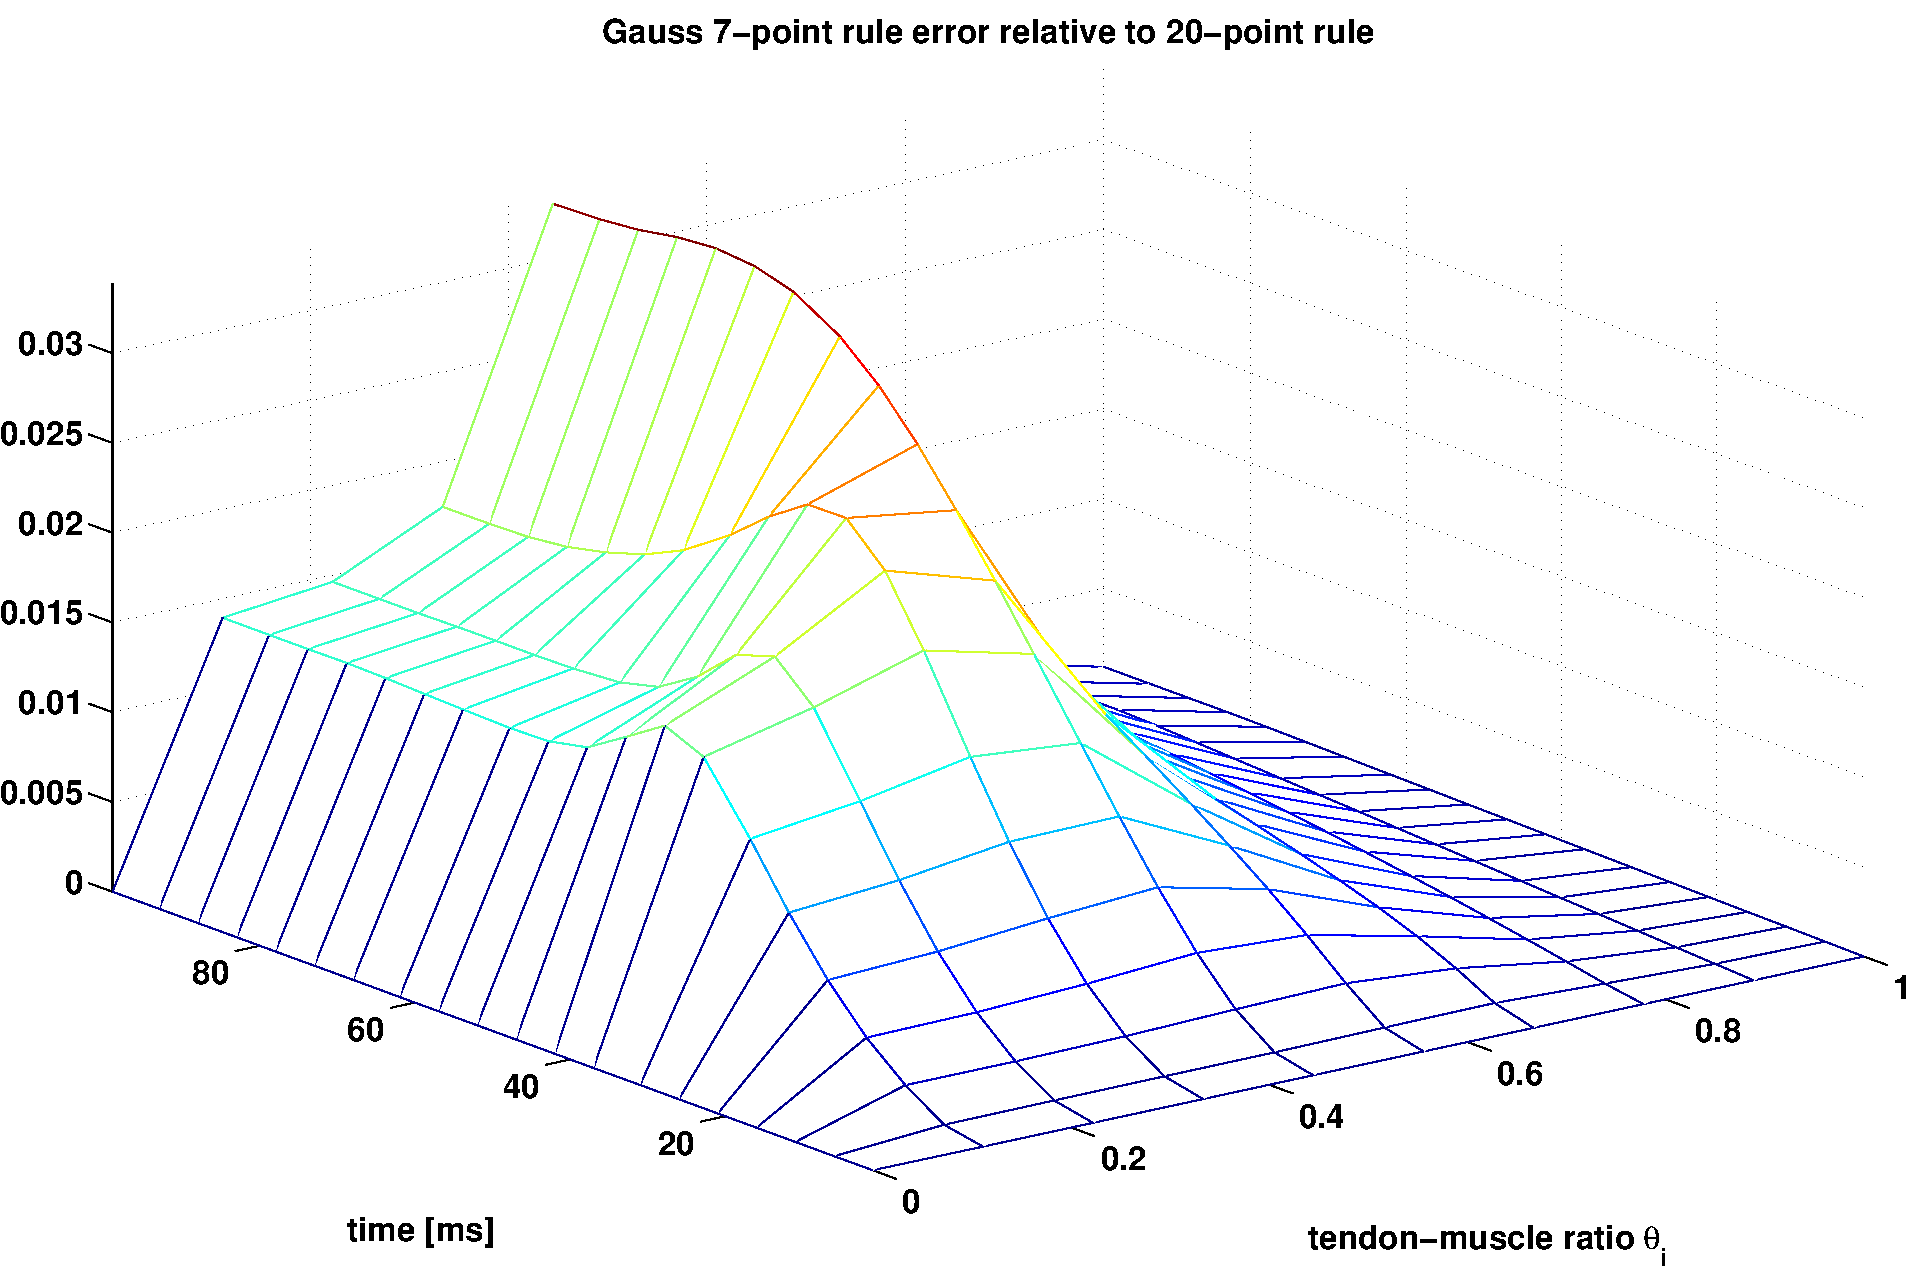
\includegraphics[width=\half]{geo_1_gaussrule_7_err}\\
	\caption{Geometry 1: Average positions of right face (x-direction) over time and tendon/muscle ratios. Top to bottom: $3,5,7$-point Gauss rules}
	\label{fig:geo1_res_pt1}
\end{figure}
\begin{figure}[!ht]
	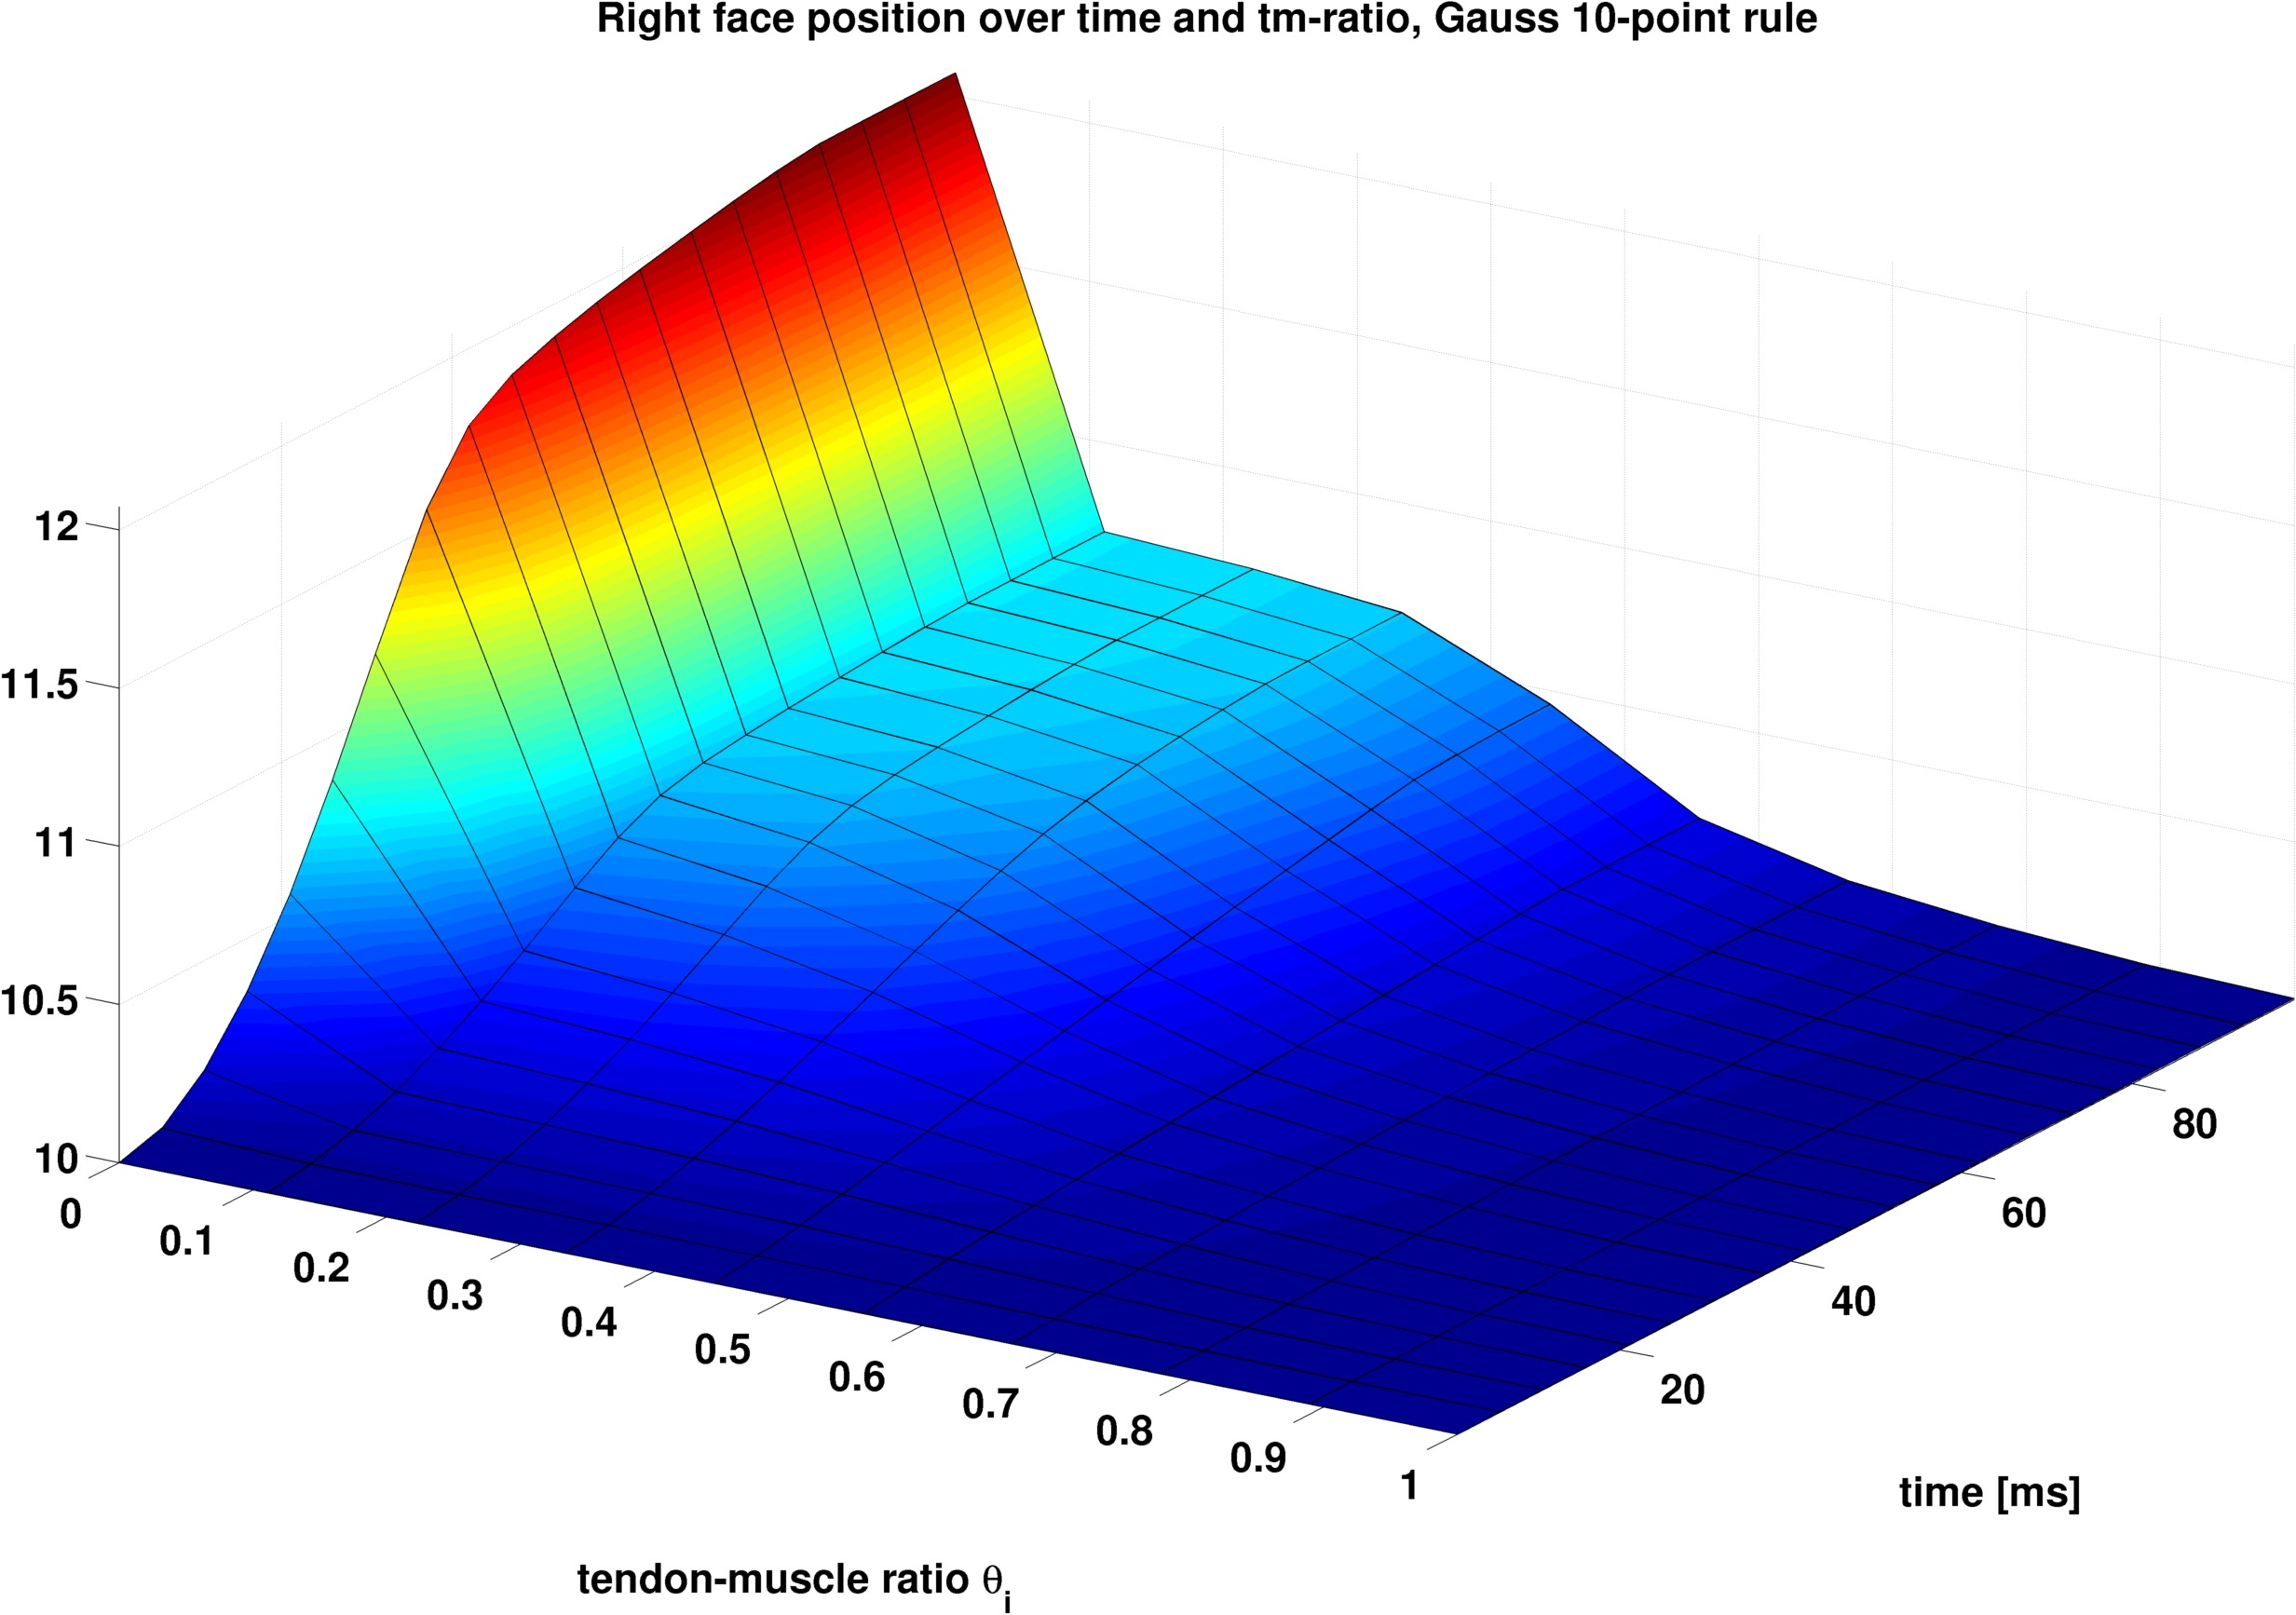
\includegraphics[width=\half]{geo_1_gaussrule_10}
% 	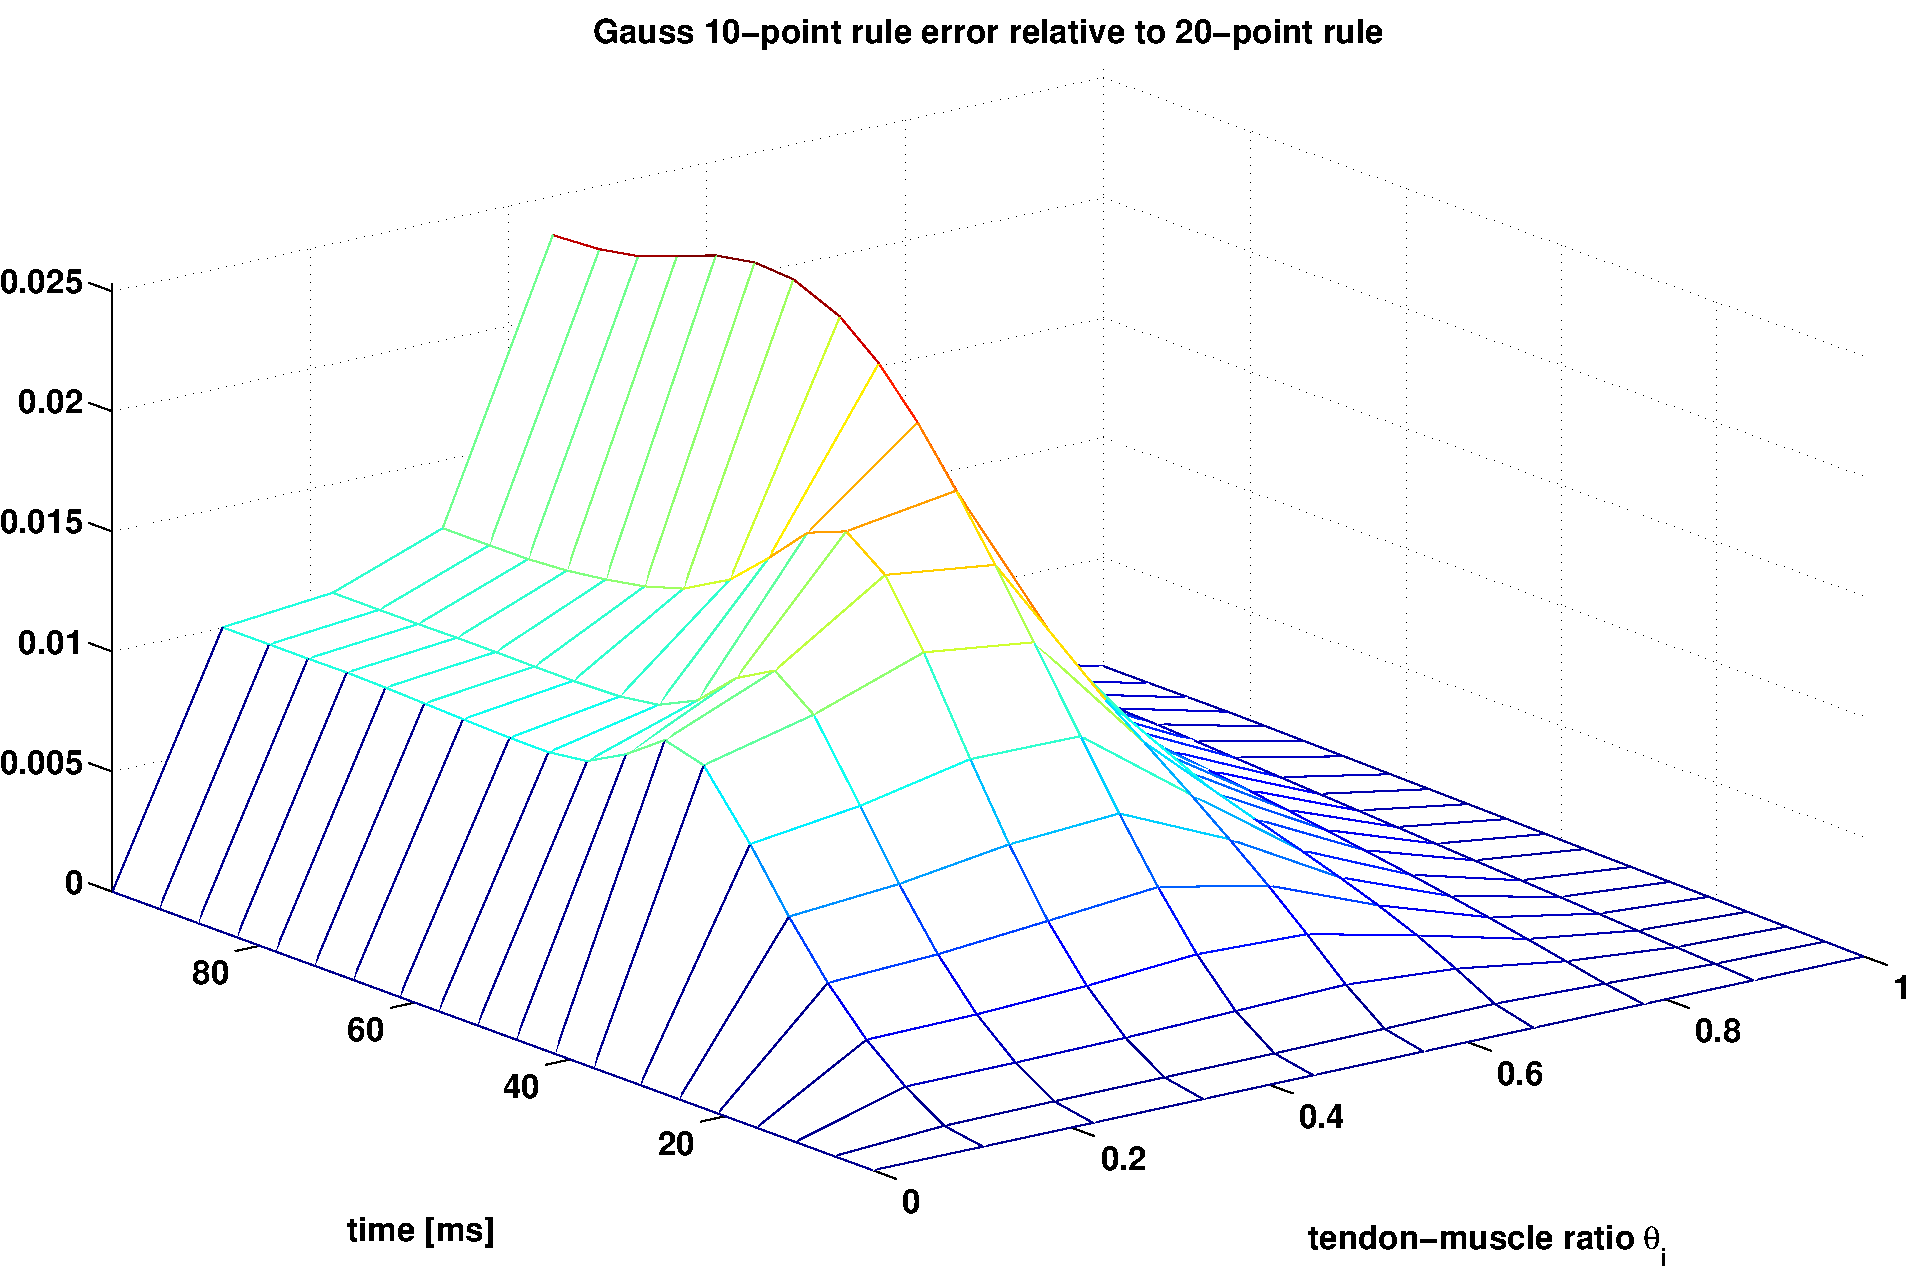
\includegraphics[width=\half]{geo_1_gaussrule_10_err}\\
% 	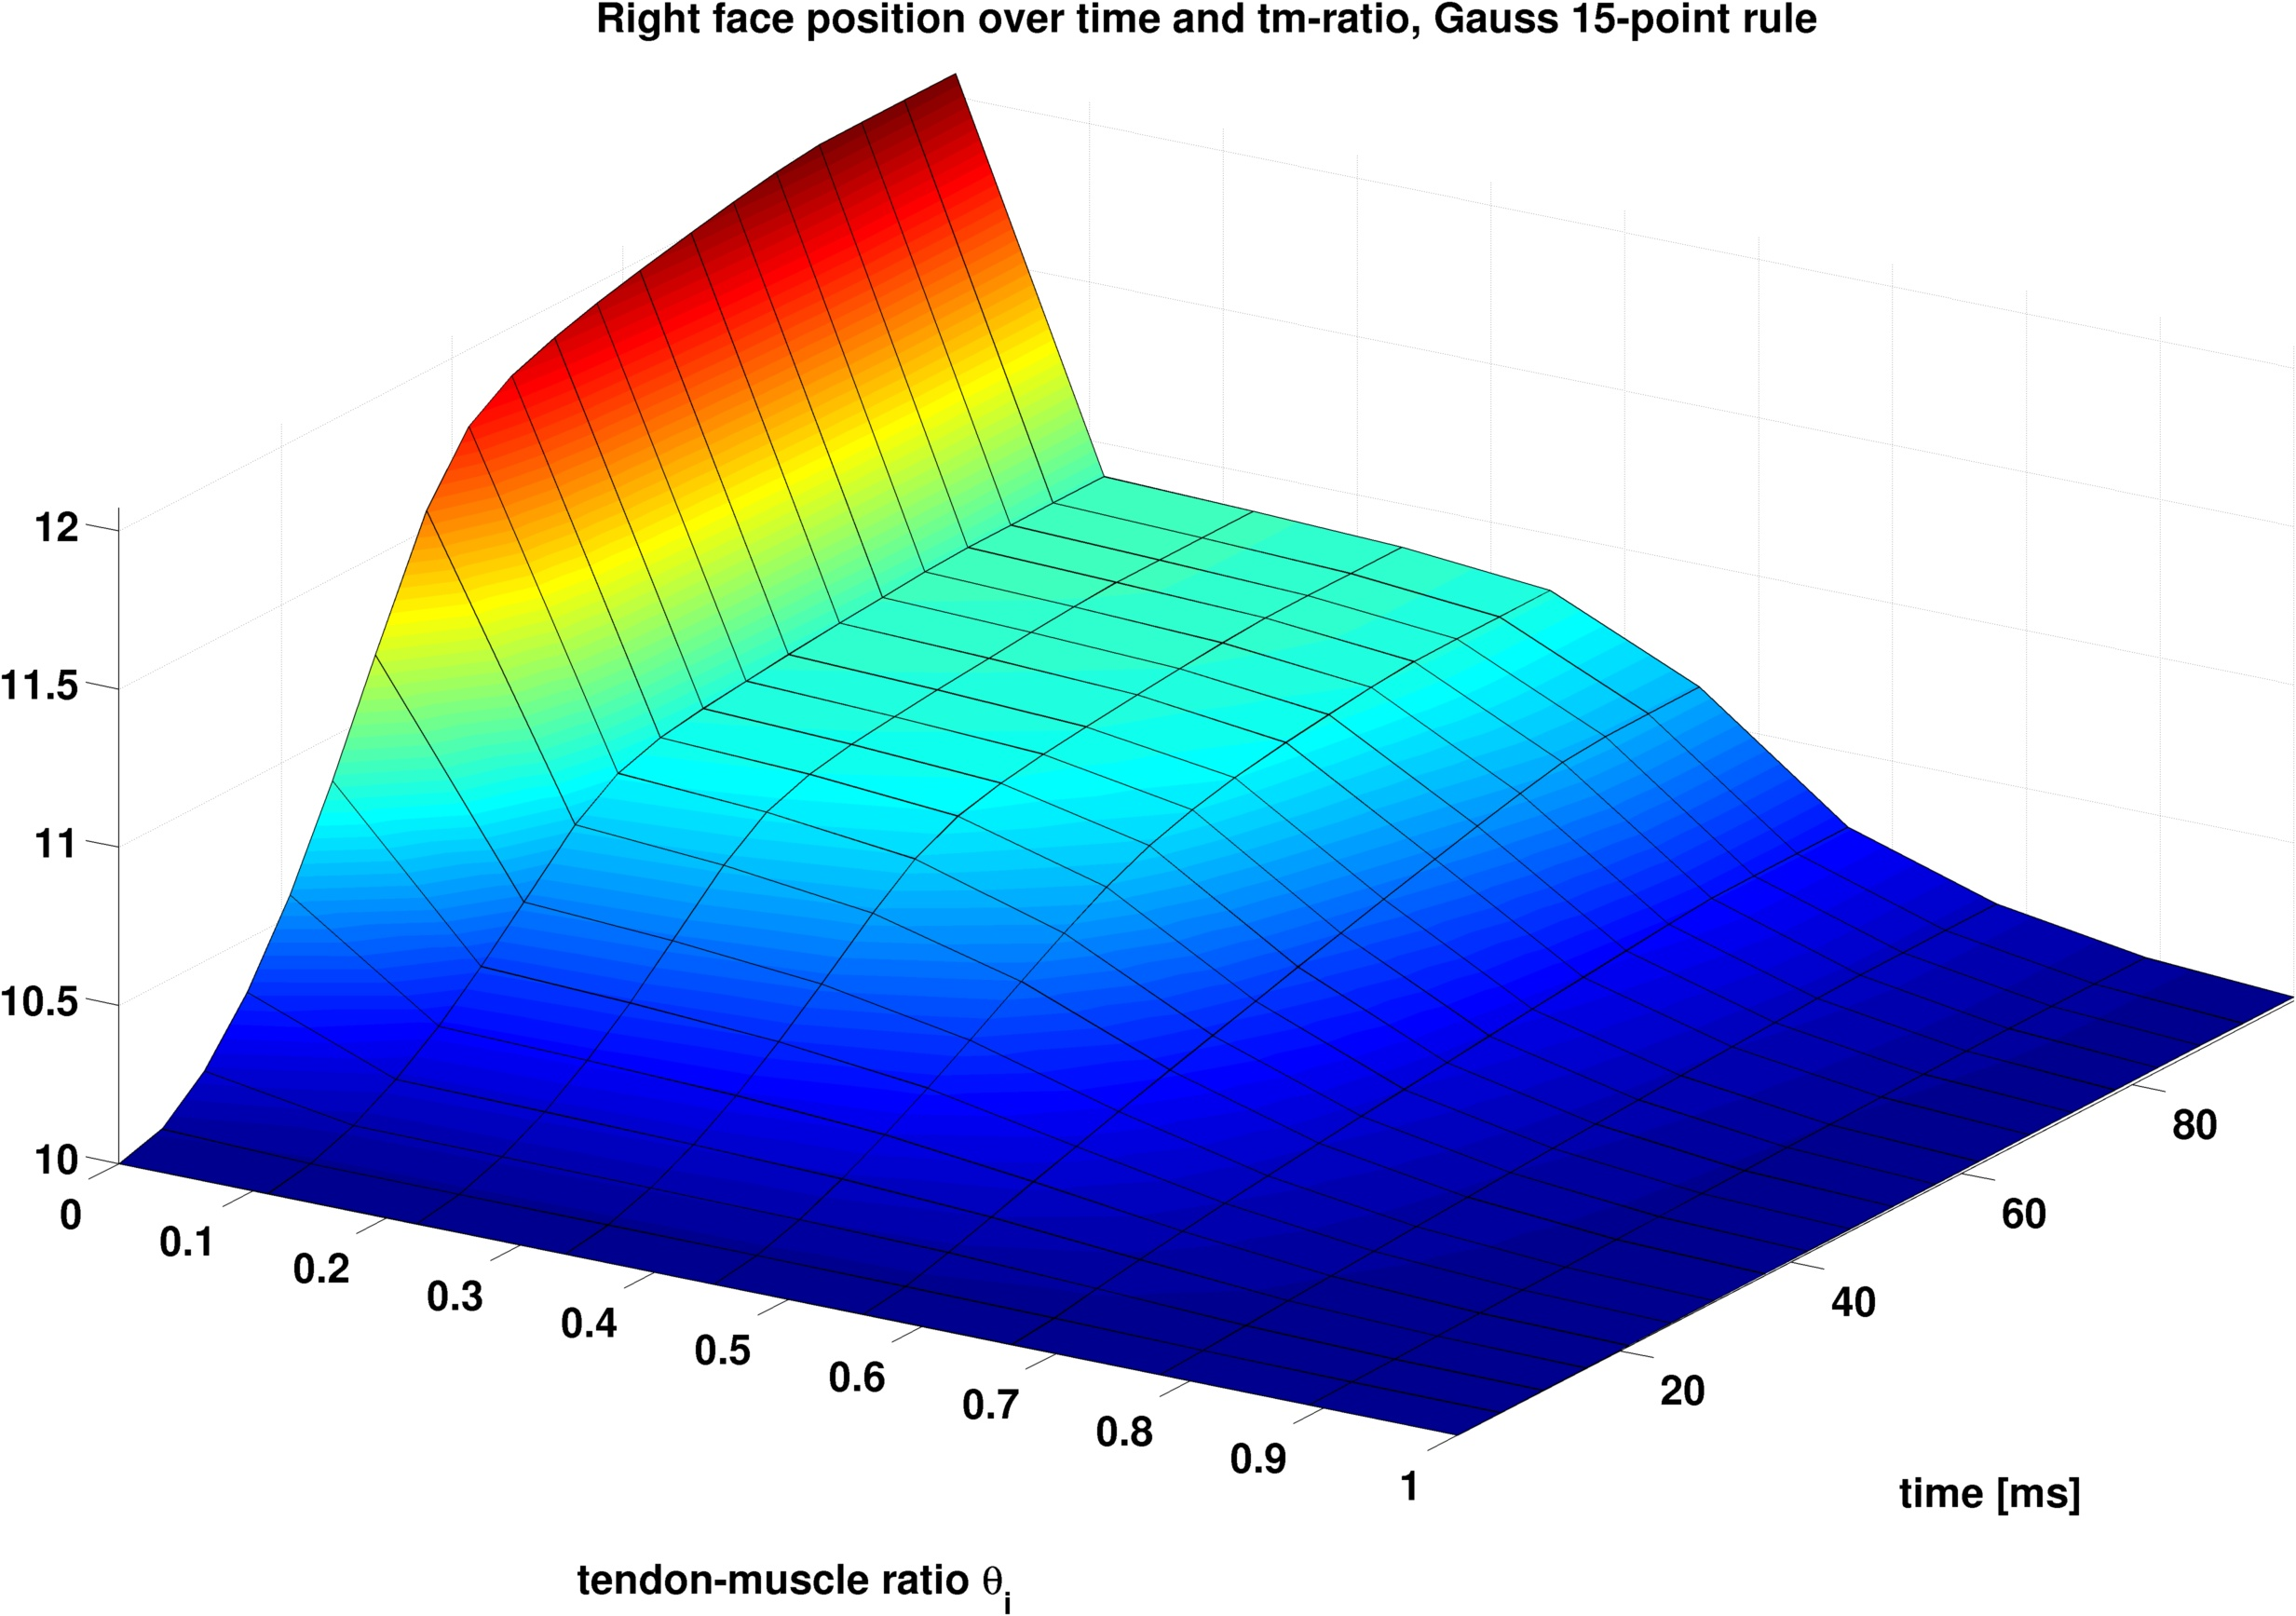
\includegraphics[width=\half]{geo_1_gaussrule_15}
% 	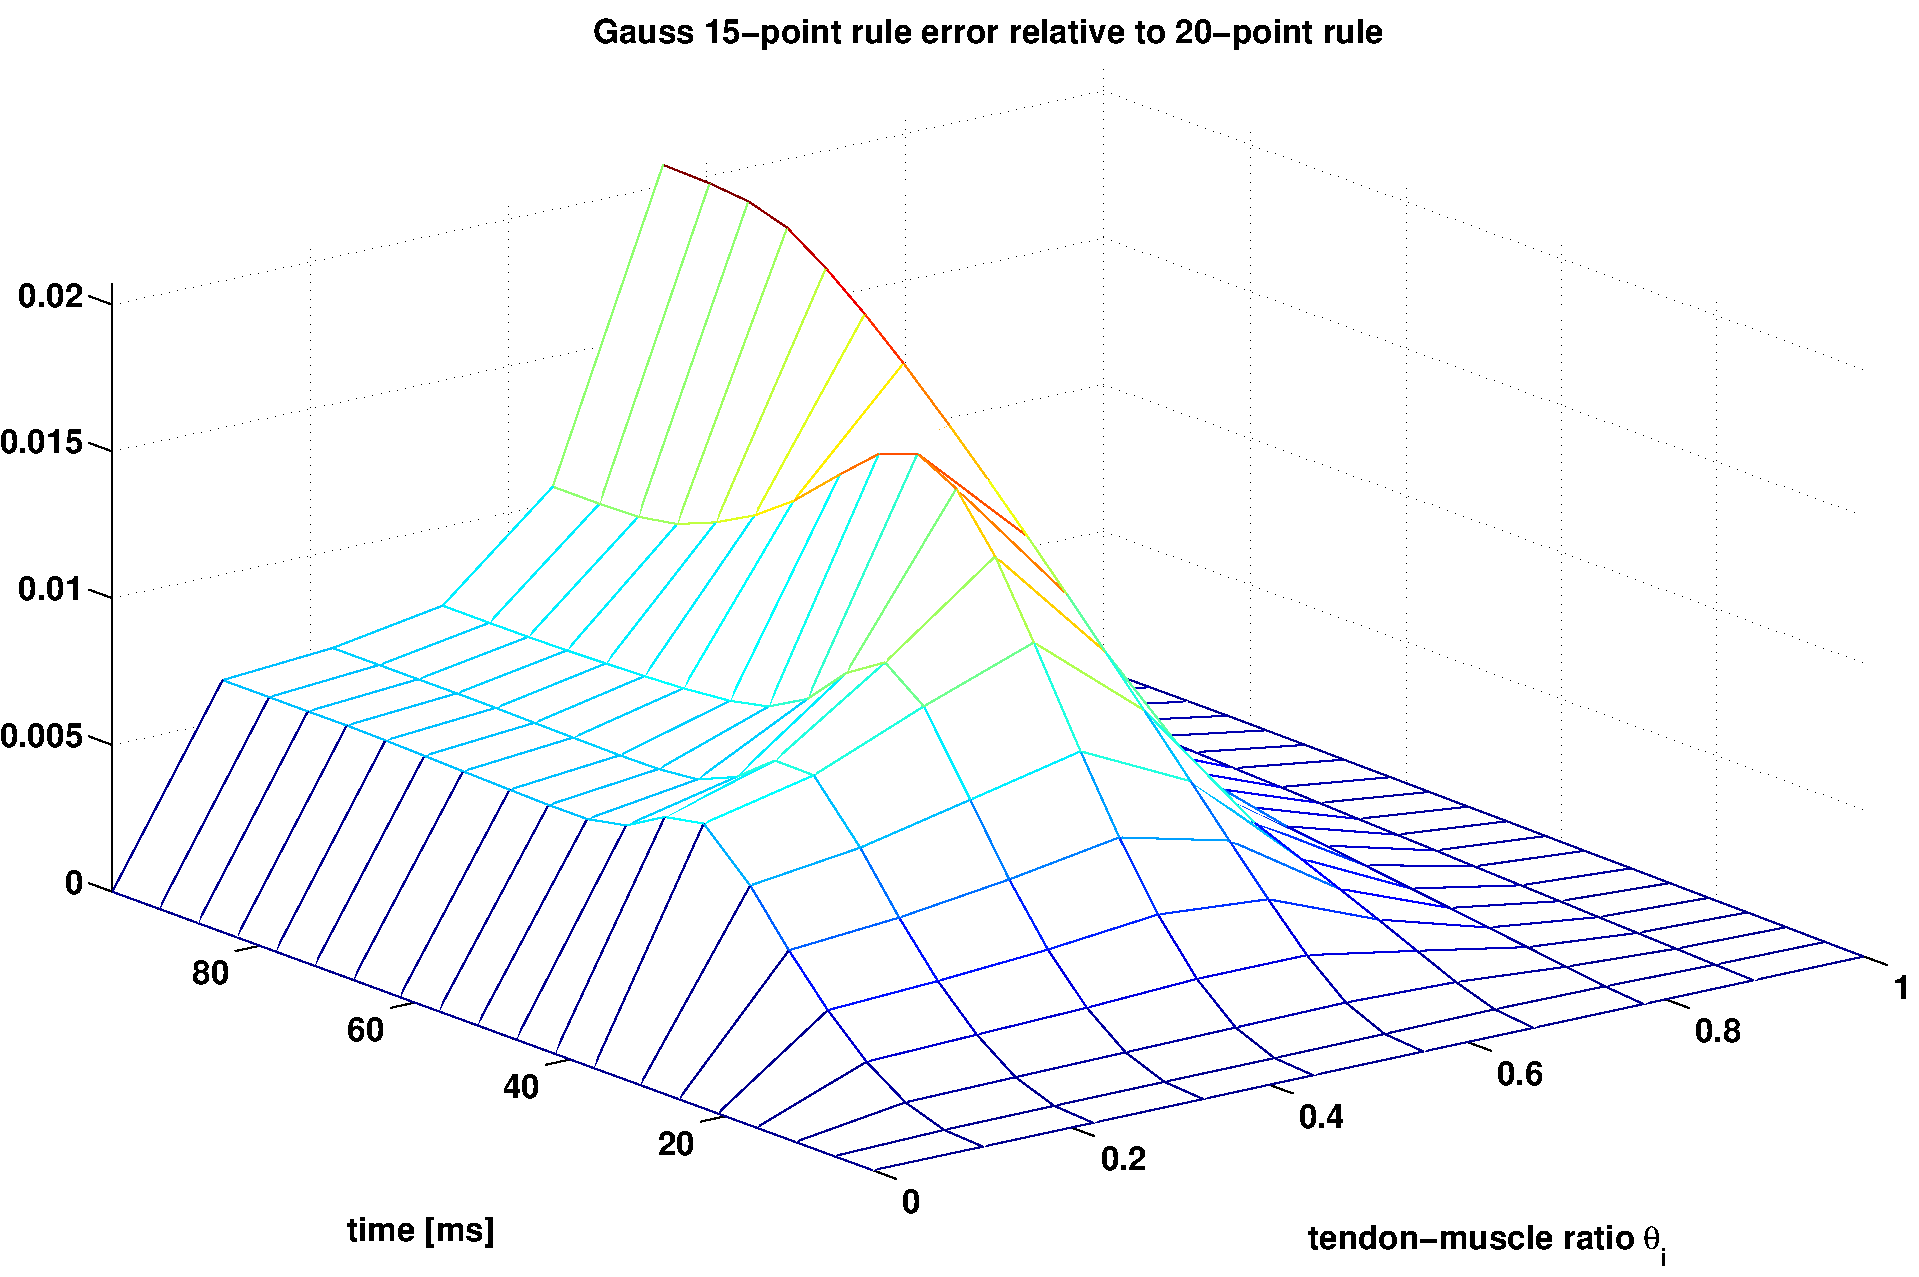
\includegraphics[width=\half]{geo_1_gaussrule_15_err}\\
% 	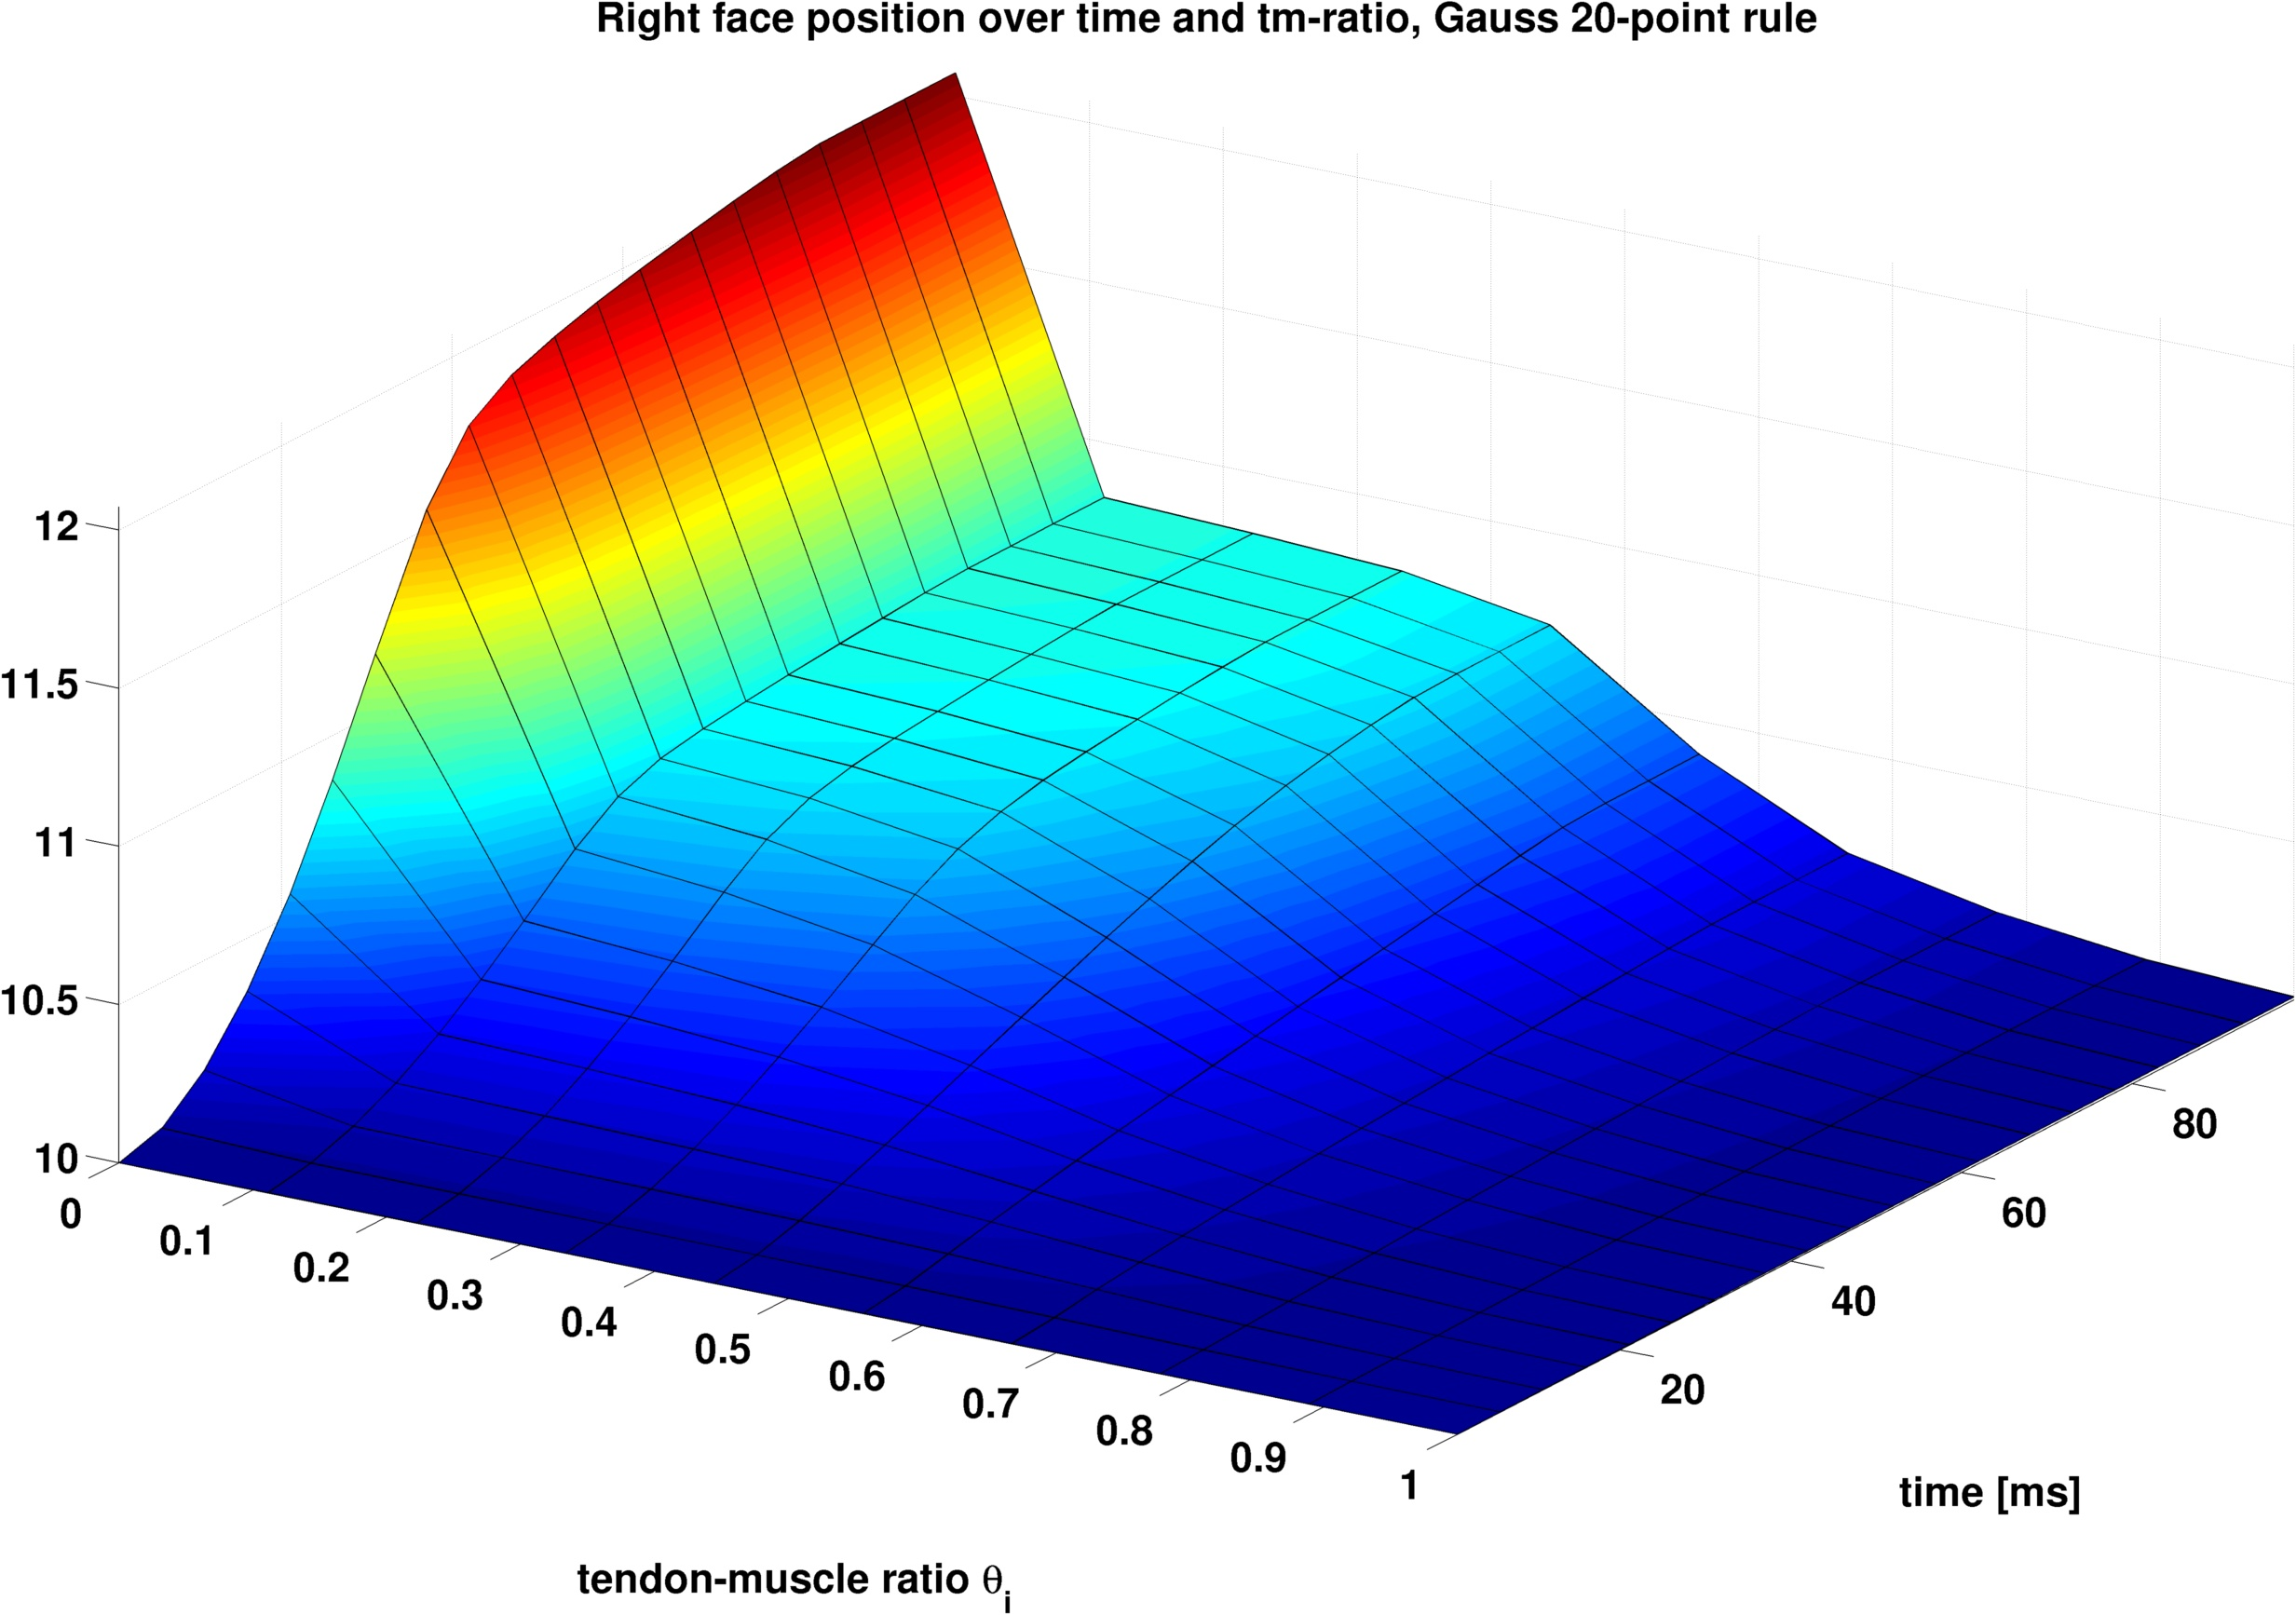
\includegraphics[width=\half]{geo_1_gaussrule_20}
% 	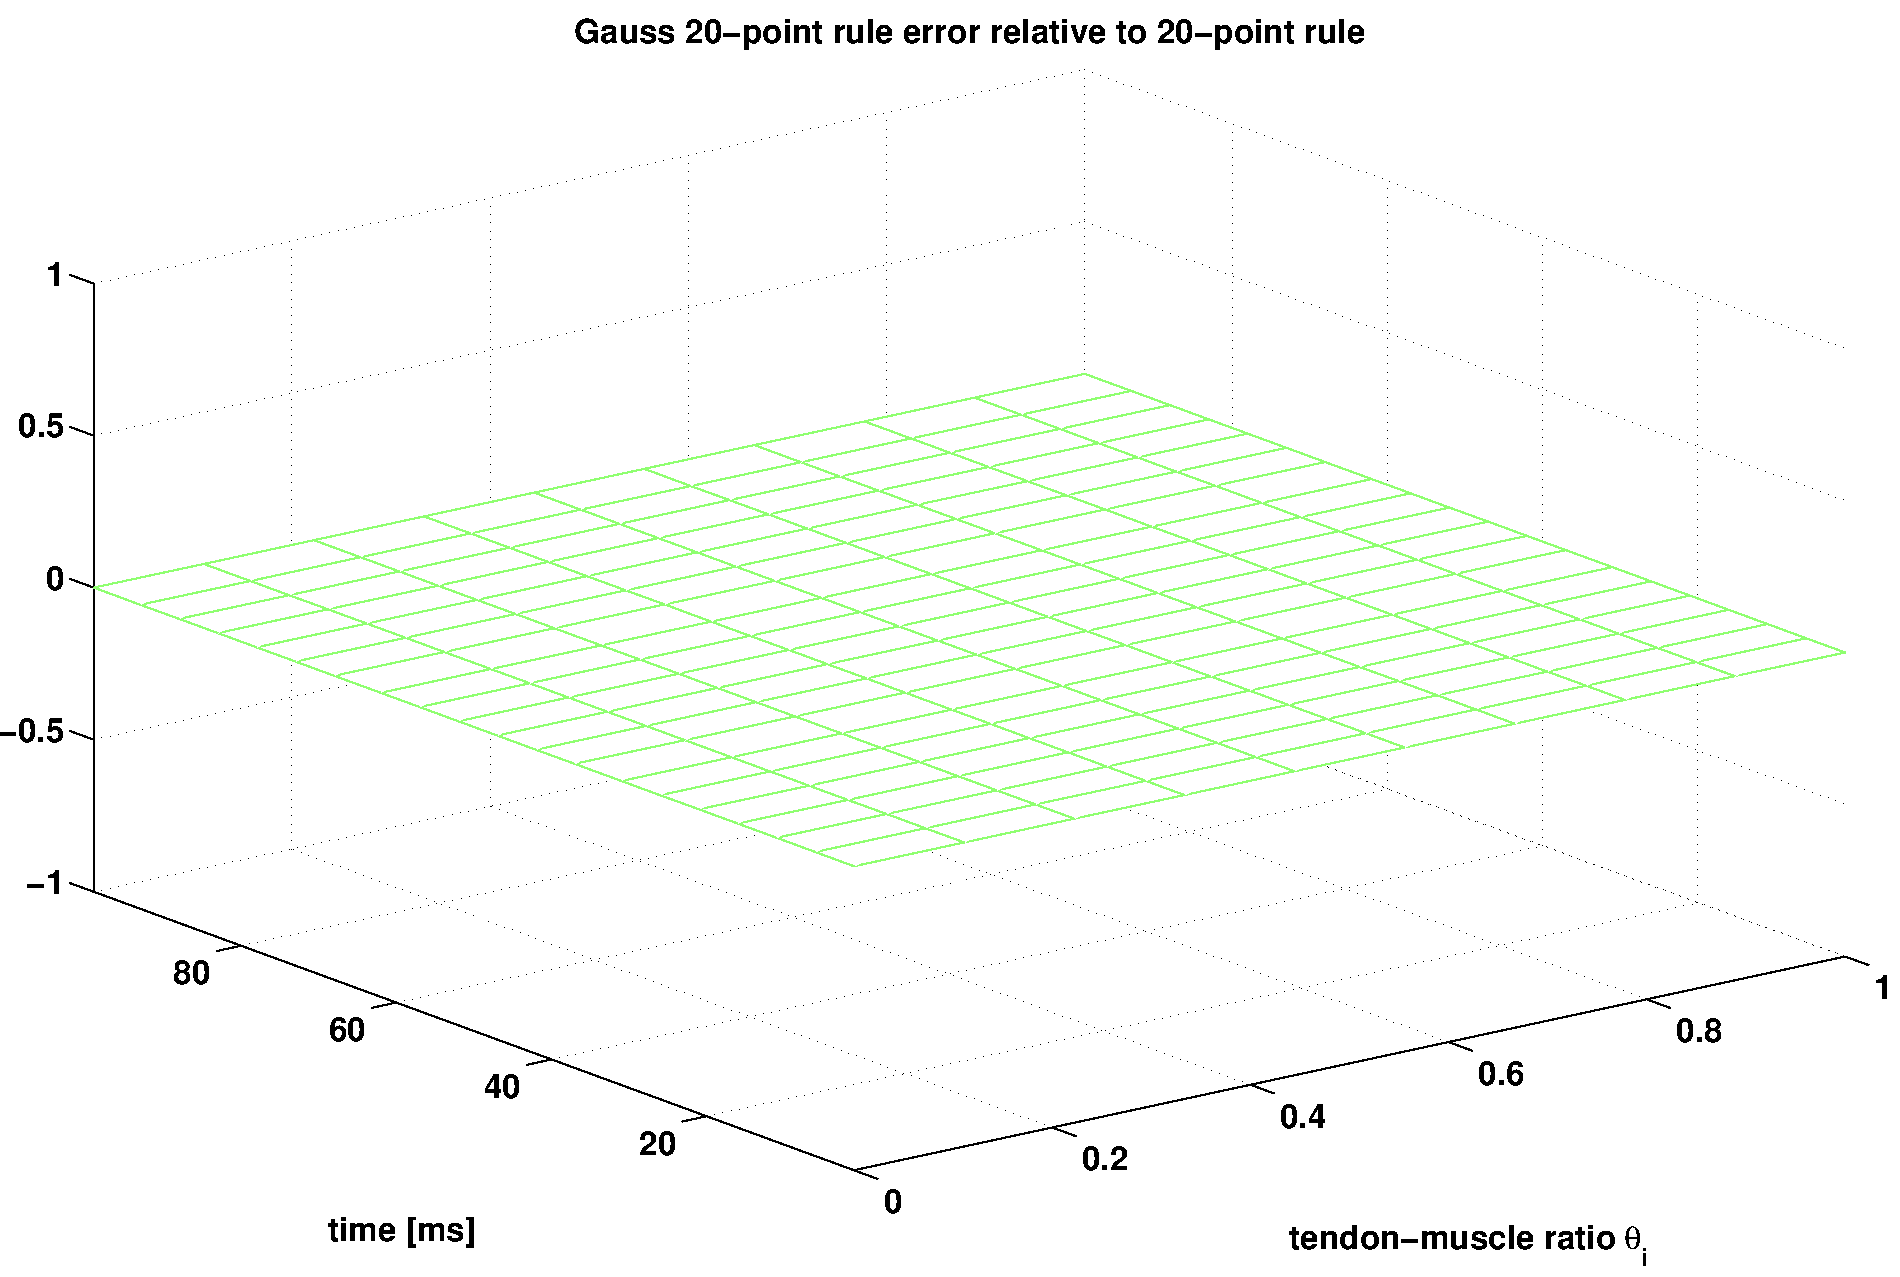
\includegraphics[width=\half]{geo_1_gaussrule_20_err}\\
	\caption{Geometry 1: Average positions of right face (x-direction) over time and tendon/muscle ratios. Top to bottom: $10,15,20$-point Gauss rules}
	\label{fig:geo1_res_pt2}
\end{figure}

Table \ref{tab:geo1_errors} shows the absolute and relative errors compared to the $20$-point Gauss integration rule results, taken over the whole time/ratio domain.
It shows that the 5-point rule is identical to the 20-point rule (up to 1\%), and clearly the three-point quadrature rule sticks out by a maximum relative
error of 20\% and mean deviation of 2\%. 
% PrintTable "Average x-Position of right face errors, config FL-1_GeoNr-1_Tag-experiments.MuscleTendonMixPullExperiment" generated on 18-May-2015 11:17:14
% Export settings: TexMathModeDetection 1, HasHeader 1, HasRowHeader 0, StripInsertedTabChars 1, IsPDF 0, TightPDF 1
\begin{table}[!htb]
	\centering
	\def\arraystretch{1.3}
	\begin{tabular}{lllll}
		Gauss rule	& Max absolute	& Mean absolute	& Max relative	& Mean relative\\
		\hline\\
		3-point		& $0.739304$	& $0.0726431$	& $0.214128$	& $0.0206339$\\
		5-point		& $0.0496134$	& $0.00468386$	& \red{$0.0136761$}	& $0.00130904$\\
		7-point		& $0.362056$	& $0.0338801$	& $0.0888703$	& $0.00845592$\\
		10-point	& $0.270046$	& $0.0253252$	& $0.0661079$	& $0.00629614$\\
		15-point	& $0.215407$	& $0.0207213$	& $0.0460988$	& $0.00440572$\\
	\end{tabular}
	\caption{Geometry 1: Errors of x-Position of right face (relative to 20-point Gauss rule)}
	\label{tab:geo1_errors}
\end{table}

Moreover, Figure \ref{fig:geo1_endpos} shows the position of the right face (averaged over nodes) at $T=99$ for different $\theta_i$ and Gauss quadrature rules.
Clearly different are the results for three-point Gauss integration, and the results for $5,15,20$-point rules are very similar.
The integration rules using $7$ and $10$ points are alike; it is unclear which rule is the most accurate, however, the accordance of $15$ and $20$-point
rules indicate that the $5$-point rule seems the best tradeoff between cost and accuracy.
\begin{figure}[!ht]
	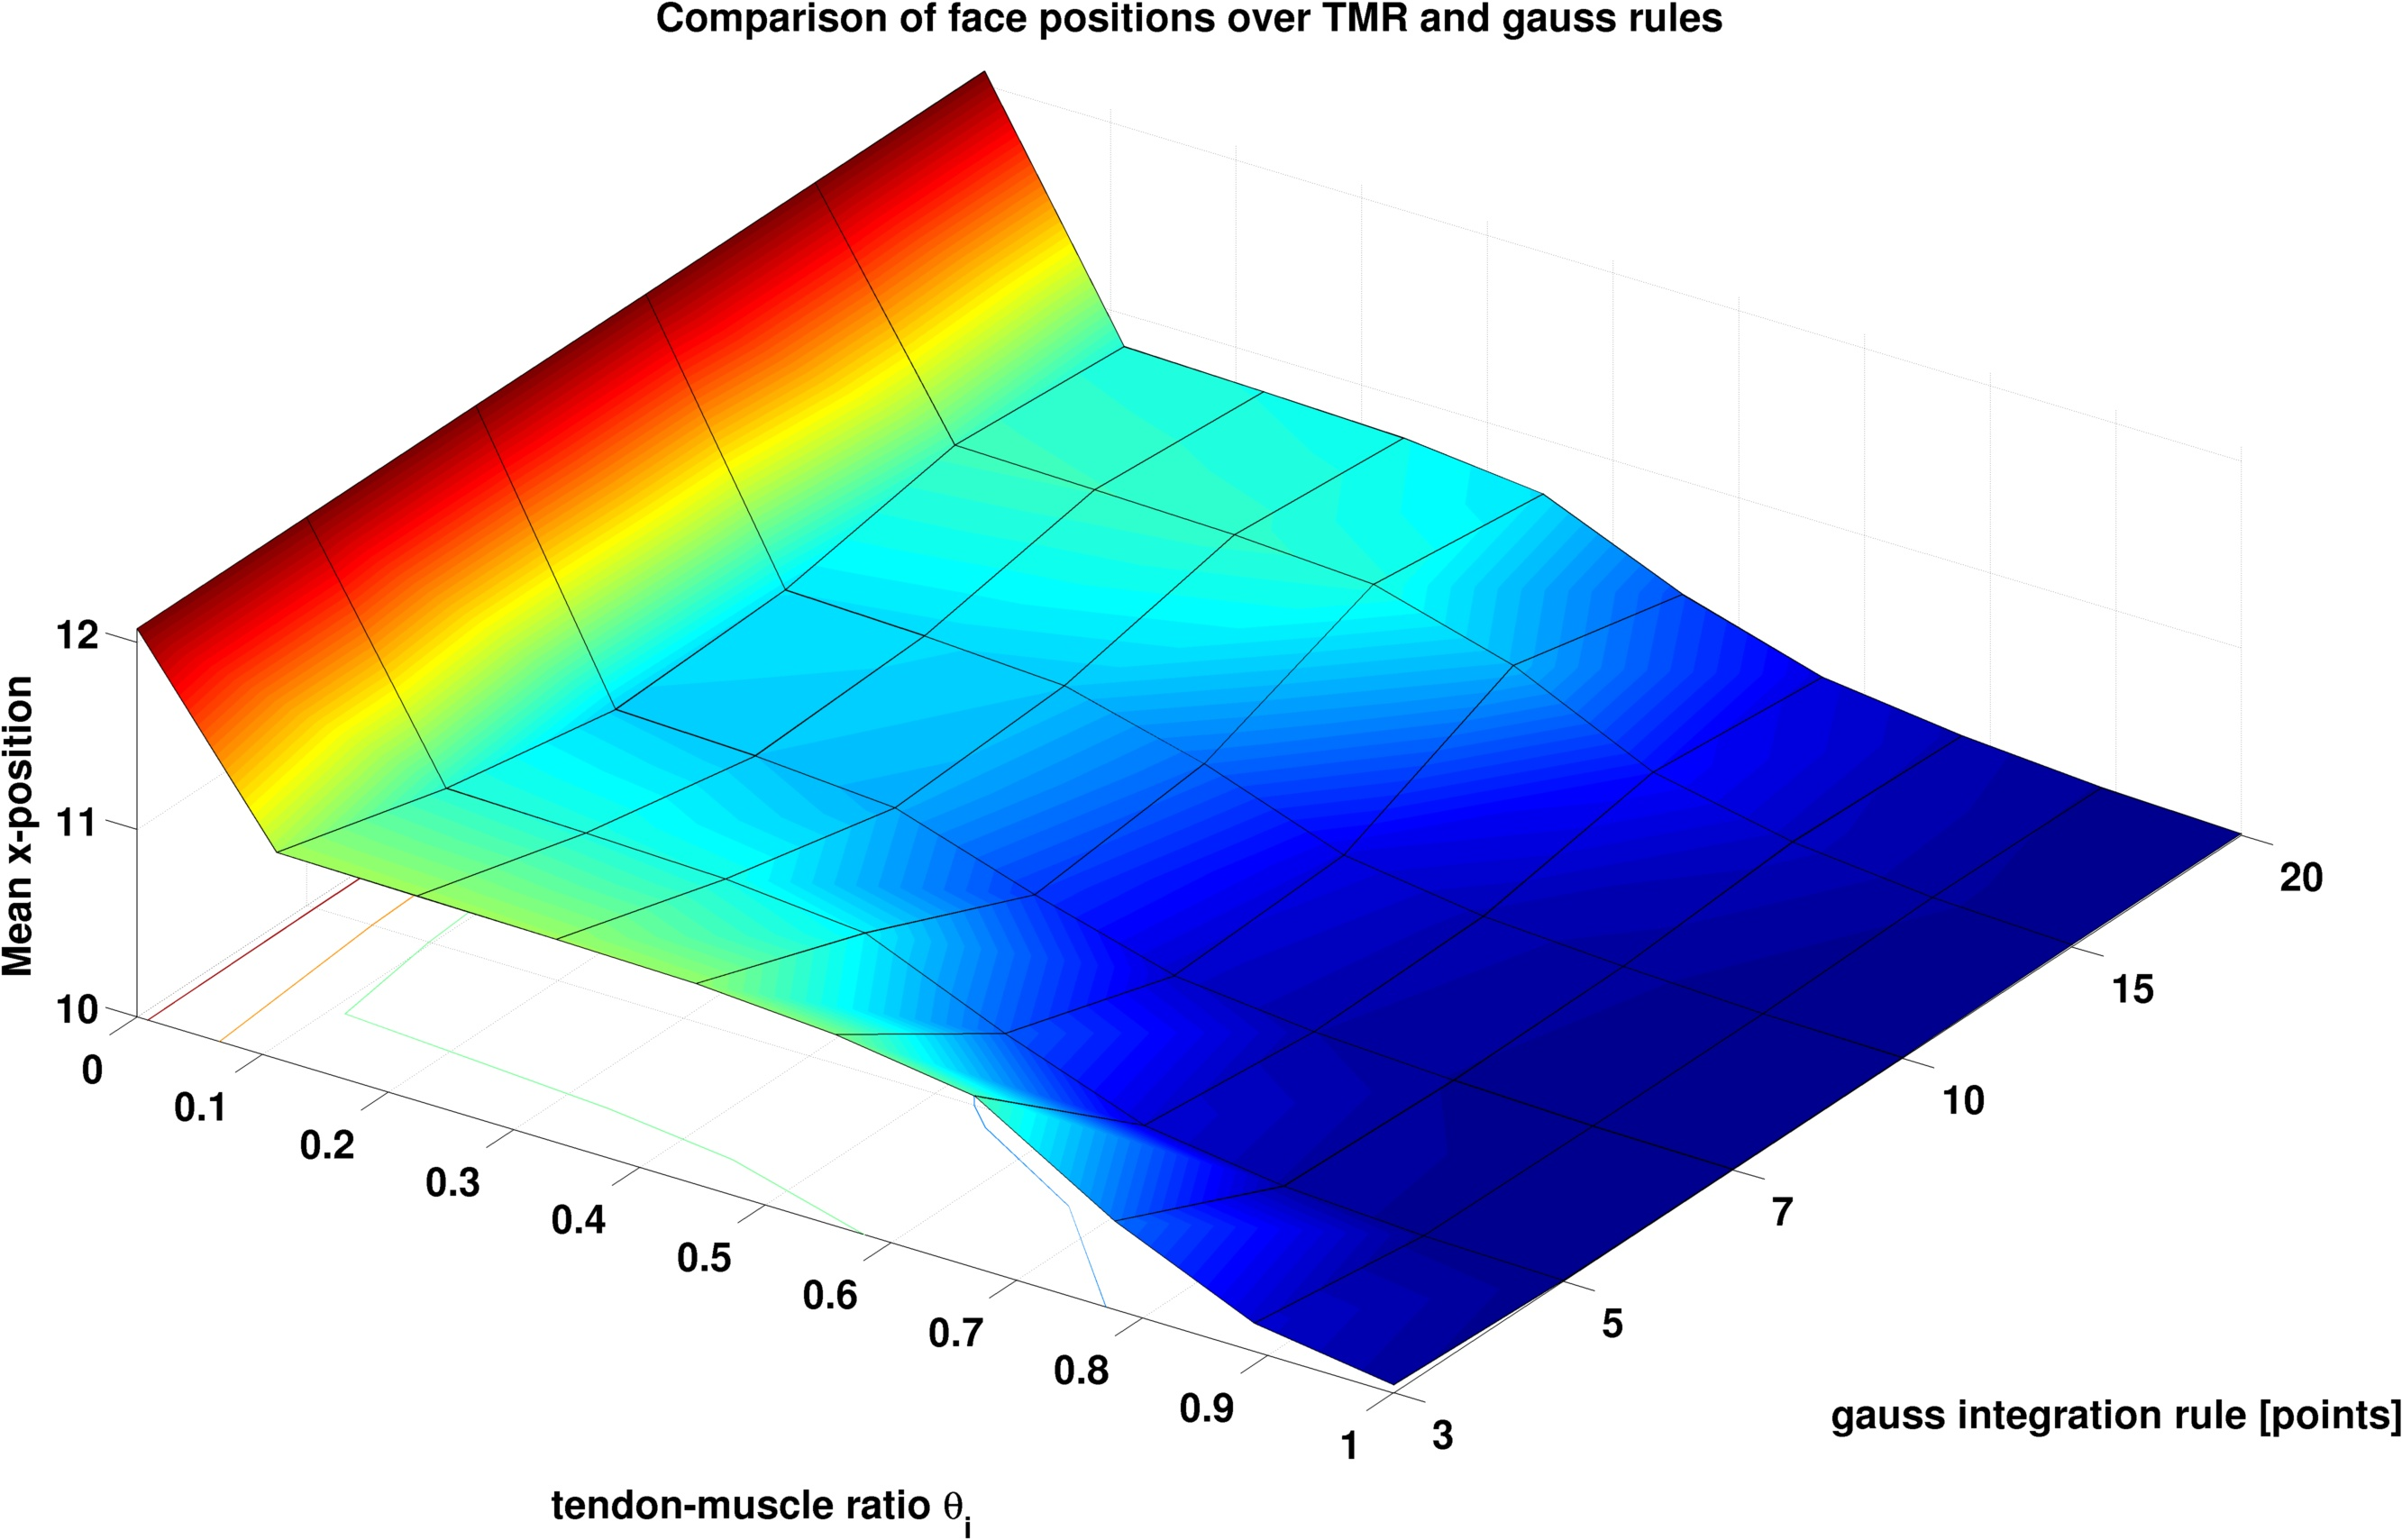
\includegraphics[width=\half]{geo_1_endpos}
	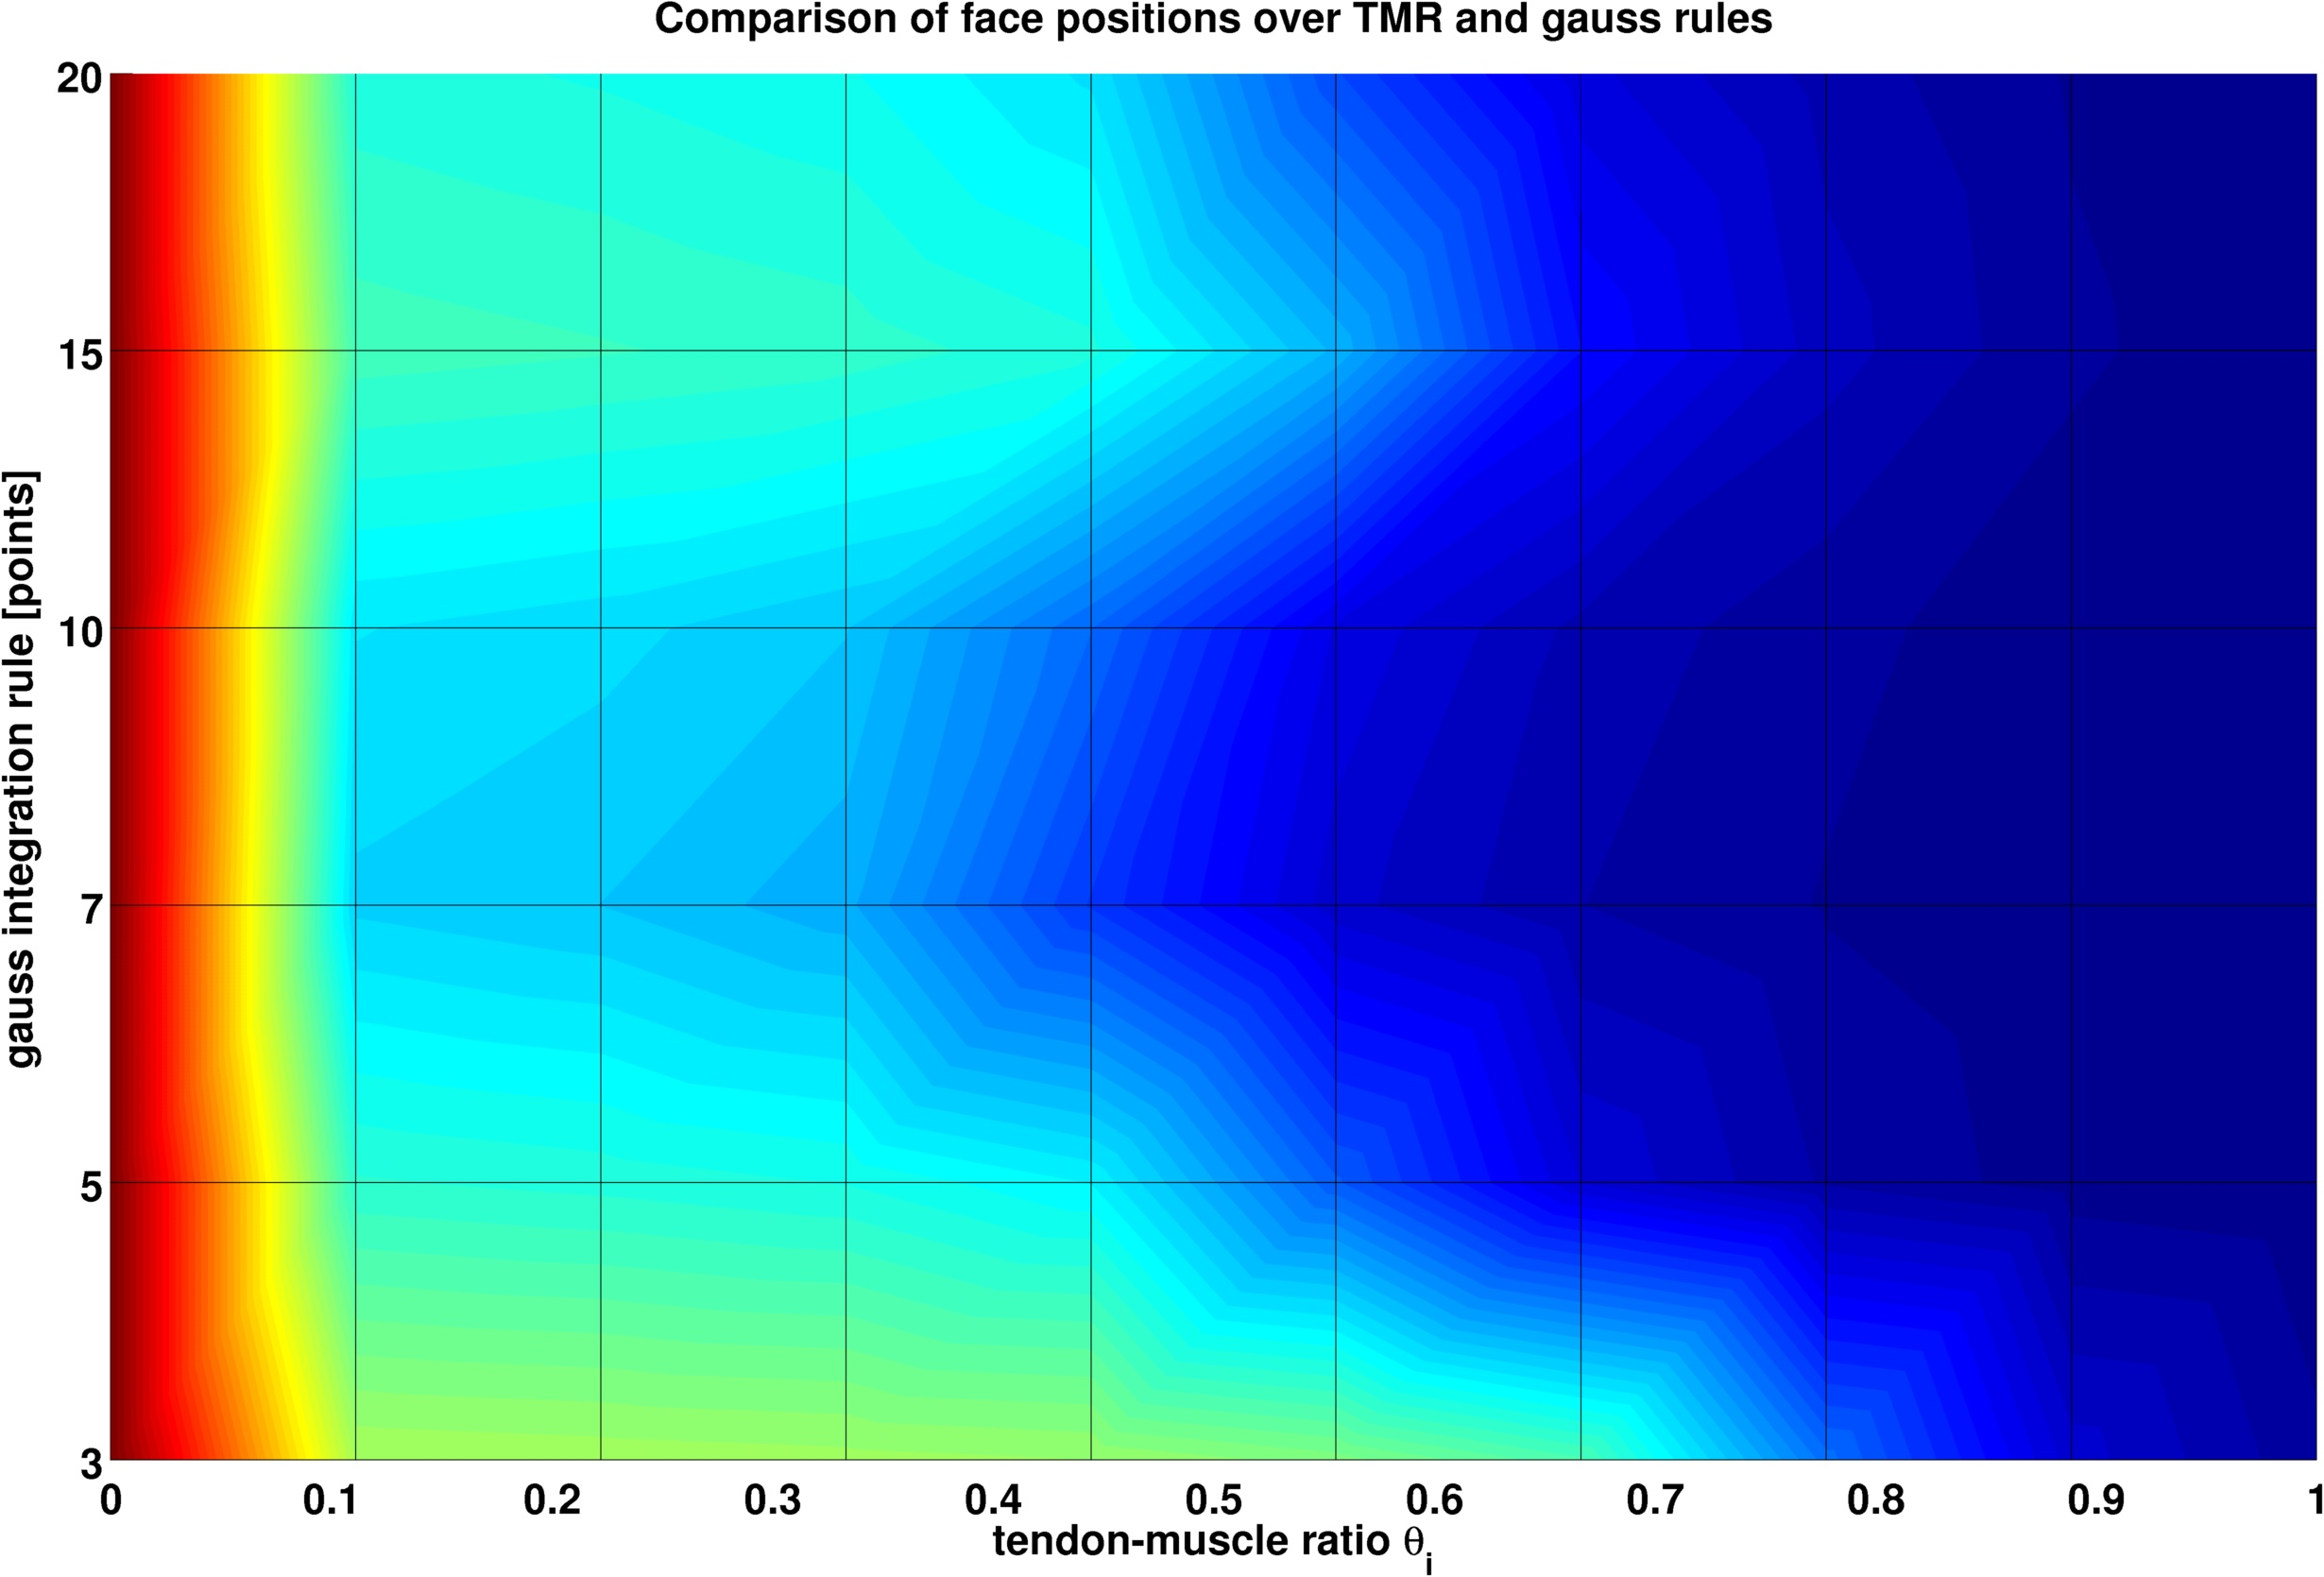
\includegraphics[width=\half]{geo_1_endpos_copy}
	\caption{Geometry 1: Average positions of right face (x-direction) over tendon/muscle ratios and quadrature rules (two view angles)}
	\label{fig:geo1_endpos}
\end{figure}

\subsubsection{Two element case}
For two elements, the results are almost identical for any integration rule, only the $3$-point rule sticks out
Figure \ref{fig:geo2_res} shows the averaged $x$-positions over time for different ratios.
\begin{figure}[!ht]
	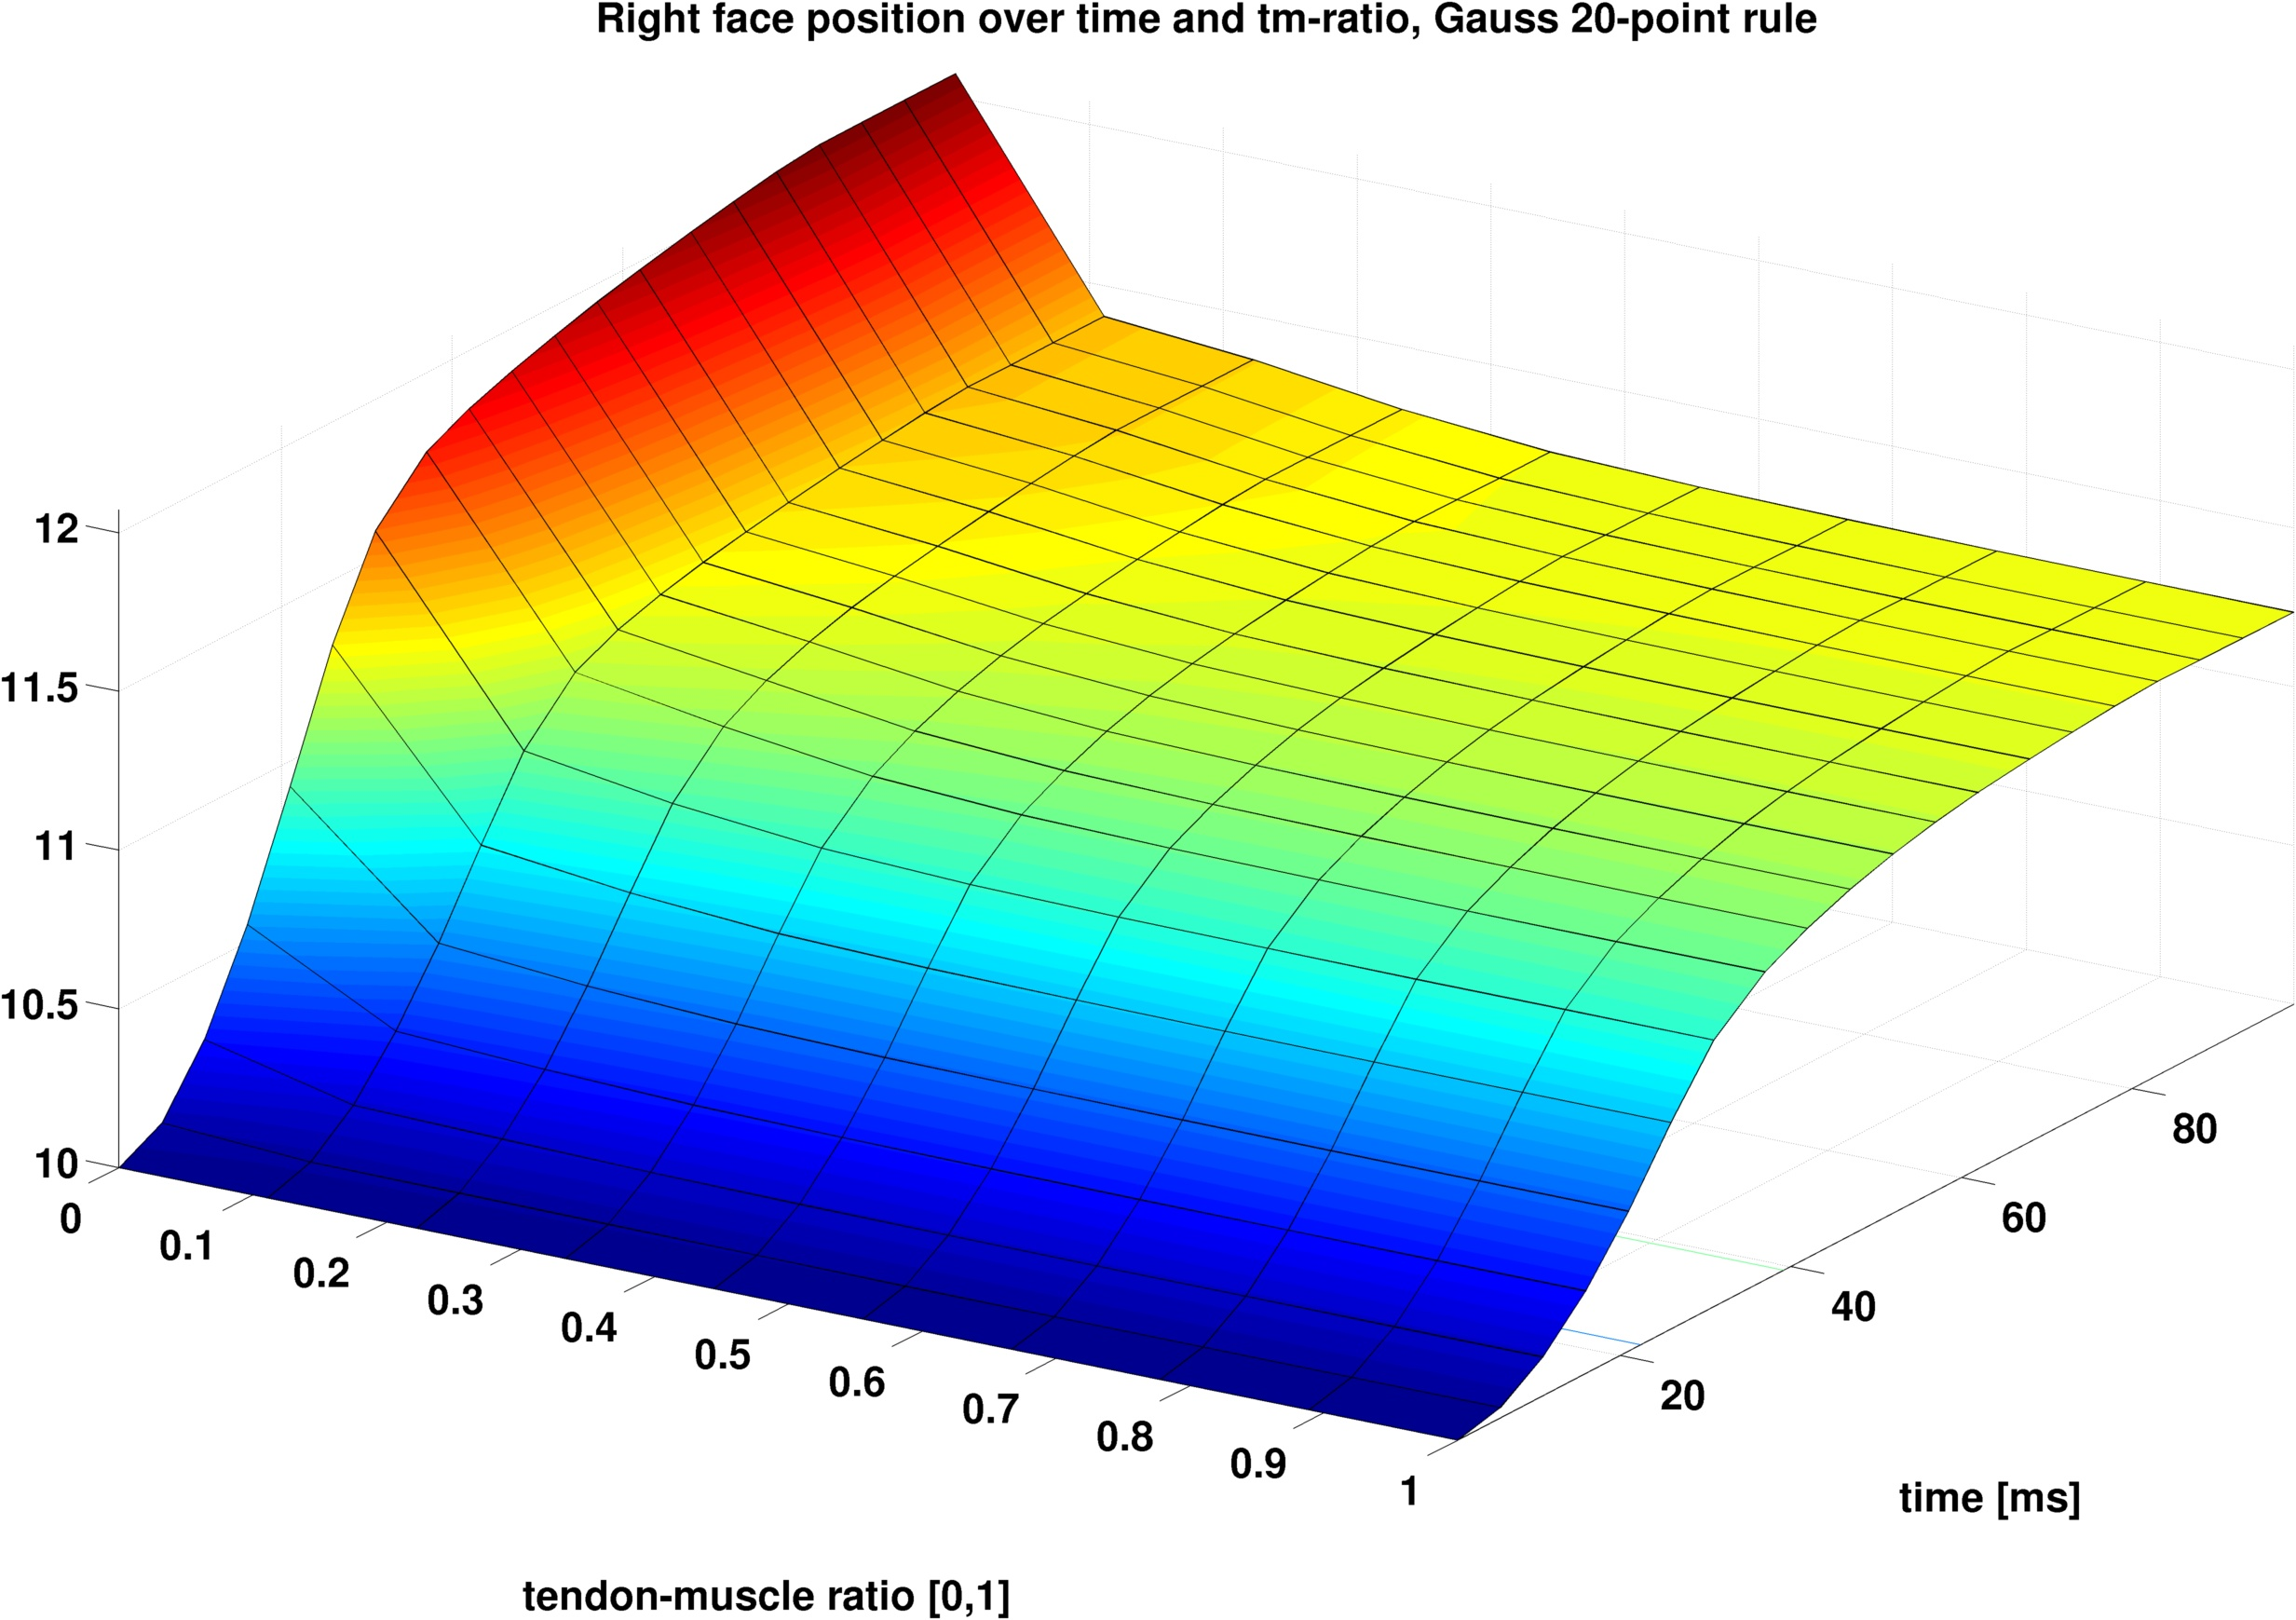
\includegraphics[width=\textwidth]{geo_2_gaussrule_20}
	\caption{Geometry 2: Average positions of right face (x-direction) over time and tendon/muscle ratios for $20$-point Gauss integration}
	\label{fig:geo2_res}
\end{figure}
Figure \ref{fig:geo2_endpos} shows the averaged $x$-positions at $T=99$ over different ratios and integration rules. 
\begin{figure}[!ht]
	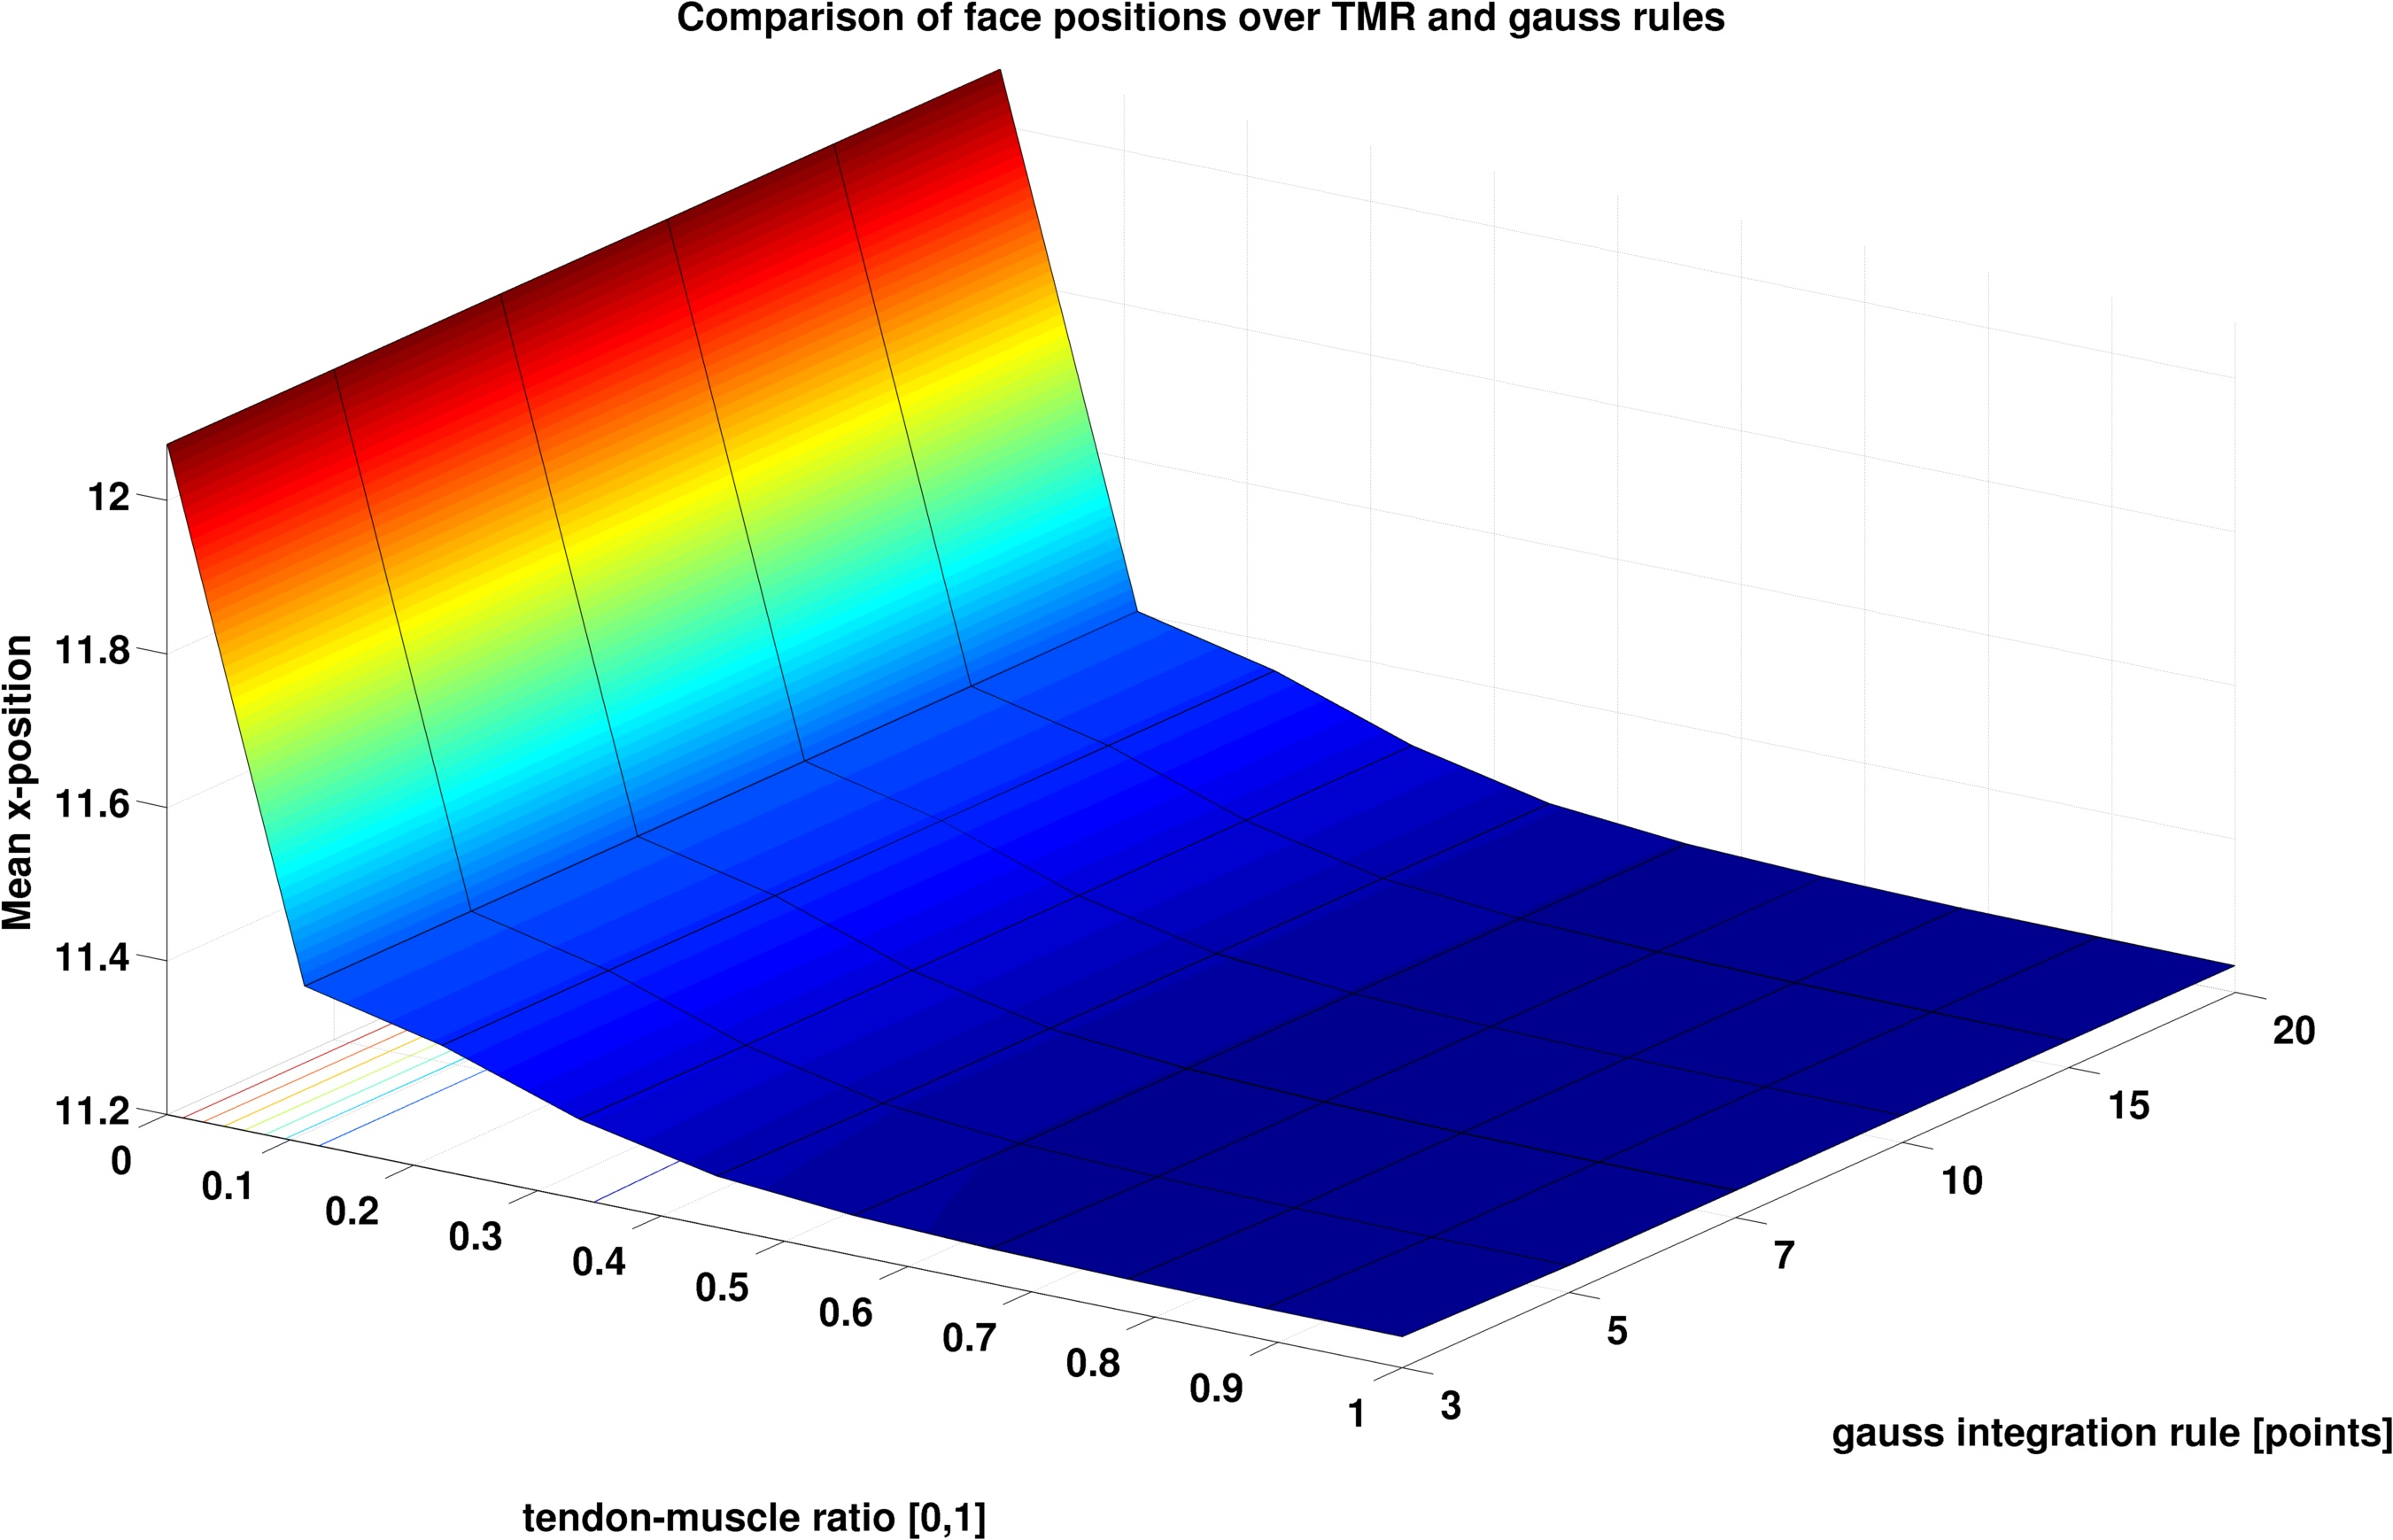
\includegraphics[width=\half]{geo_2_endpos}
	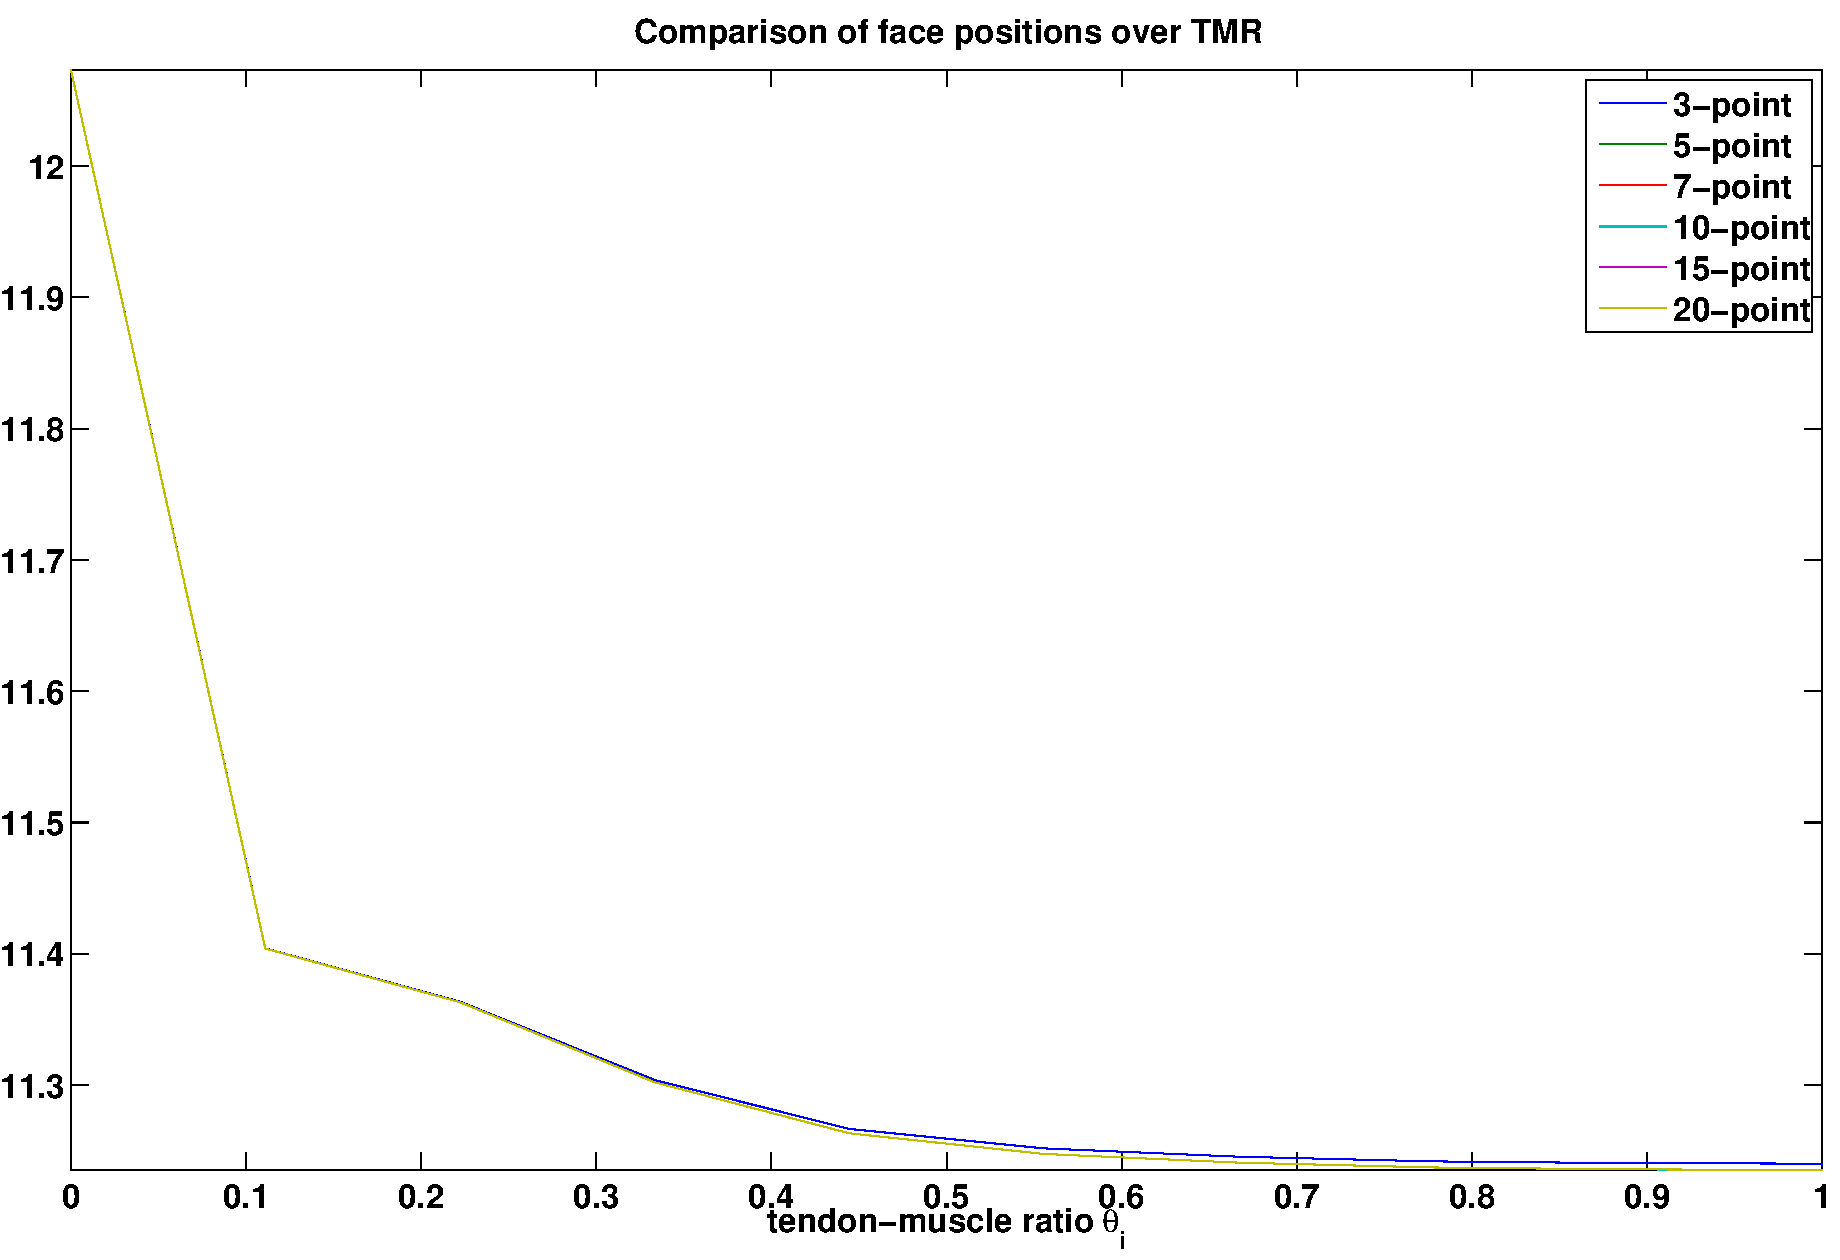
\includegraphics[width=\half]{geo_2_endpos_2d}
	\caption{Geometry 2: Average positions of right face (x-direction) at $T=99$}
	\label{fig:geo2_endpos}
\end{figure}

% PrintTable "Average x-Position of right face errors, config FL-1_GeoNr-2_Tag-experiments.MuscleTendonMixPullExperiment" generated on 18-May-2015 11:18:45
% Export settings: TexMathModeDetection 1, HasHeader 1, HasRowHeader 0, StripInsertedTabChars 1, IsPDF 0, TightPDF 1
\begin{table}[!htb]
	\centering
	\def\arraystretch{1.3}
	\begin{tabular}{lllll}
		Gauss rule	& Max absolute	& Mean absolute	& Max relative	& Mean relative\\
		\hline\\
		3-point		& $0.00478031$	& $0.00042547$	& $0.0013836$	& $0.000123551$\\
		5-point		& $0.000142599$	& $1.36352e-05$	& $1.19539e-05$	& $1.09526e-06$\\
		7-point		& $0.000242614$	& $2.41771e-05$	& $1.17654e-05$	& $1.11555e-06$\\
		10-point	& $0.000216248$	& $2.15497e-05$	& $1.03183e-05$	& $9.75682e-07$\\
		15-point	& $0.000165331$	& $1.58088e-05$	& $7.2589e-06$	& $6.85693e-07$\\
	\end{tabular}
	\caption{Geometry 2: Errors of averaged x-Position of right face}
\end{table}